\documentclass[11pt,a4paper]{article}

\usepackage{amsfonts,amssymb,amsmath}
\usepackage[margin=1in]{geometry}
\usepackage[none]{hyphenat}
\usepackage{graphicx}
\usepackage{fancyhdr}
\usepackage{float}
\usepackage{color}
\usepackage{xcolor}
\usepackage{tikz}
% Straight quotes in verbatim, so that code copied from the notes runs.
\usepackage{upquote}
\usepackage[nottoc,notlot,notlof]{tocbibind}

\usetikzlibrary{arrows.meta,shapes,positioning}

\parindent 0ex
% hyphenat[none] forbids hyphenation, so give TeX room to stretch a line
% instead of letting it run into the margin.
\setlength{\emergencystretch}{3em}
\setlength{\parskip}{0.55\baselineskip}
\setlength{\abovedisplayskip}{0.5\baselineskip}
\setlength{\belowdisplayskip}{0.5\baselineskip}
\setlength{\abovedisplayshortskip}{0.25\baselineskip}
\setlength{\belowdisplayshortskip}{0.25\baselineskip}
\numberwithin{equation}{section}

\pagestyle{fancy}
\fancyfoot[C]{\thepage}
\fancyhead{}
\fancyhead[R]{\rightmark}
\renewcommand{\headrulewidth}{0pt}

% Upright operator names.
\DeclareMathOperator{\tr}{tr}
\DeclareMathOperator{\rank}{rank}
\DeclareMathOperator{\sgn}{sgn}
\DeclareMathOperator{\Real}{Re}
\DeclareMathOperator{\Imag}{Im}

% Theorem environments.
\usepackage{amsthm}
\theoremstyle{definition}
% One shared counter running section.subsection.n, as in the other courses here.
\newtheorem{thm}{Theorem}[subsection]
\newtheorem{defn}[thm]{Definition}
\newtheorem{exa}[thm]{Example}
\newtheorem{prop}[thm]{Proposition}
\newtheorem{coro}[thm]{Corollary}
\newtheorem{lem}[thm]{Lemma}
% An "In software" panel: the Python commands, the output they print, and how to read
% it. The web build gives these their own colour (build.py tags the type from
% the label, and "Software" is tested before every other label).
\newtheorem{software}[thm]{Software}
\newtheorem*{note}{Note}
\newtheorem*{remark}{Remark}
\newtheorem{problemx}{Problem}[subsection]
\newenvironment{problem}{\begin{problemx}}{\end{problemx}}
\newenvironment{solution}
  {\renewcommand{\qedsymbol}{}\begin{proof}[\textit{Solution}.]}
  {\end{proof}}
\usepackage{enumitem}
% A heading that is legal inside a theorem body, a list or a float, where
% \subsubsection is not. Same weight as \subsubsection* so the two read alike.
\newcommand{\subhead}[1]{%
  \par\medskip\noindent\textbf{#1}\par\nobreak\smallskip}

\begin{document}
% Title page depersonalised for the web, as with every other course here. The
% identity kept below is the heat equation's fundamental solution, the kernel
% from which much of the course's linear theory is built.
\begin{titlepage}
\thispagestyle{empty}
\begin{center}
\vspace*{3cm}
{\Huge\bfseries Partial Differential Equations}\\[1.2cm]
{\large Lecture Notes}\\[2.5cm]
\line(1,0){300}\\[1.5cm]
$$u_t=\kappa\,\Delta u,\qquad \Phi(x,t)=\frac{1}{(4\pi\kappa t)^{n/2}}\,e^{-|x|^2/4\kappa t}$$
\end{center}
\end{titlepage}

\tableofcontents
\thispagestyle{empty}
\clearpage
\setcounter{page}{1}

%======================================================================
\section{First-Order Equations and Characteristics}
\label{sec:characteristics}

A partial differential equation relates an unknown function of several variables to its partial derivatives. The great equations of mathematical
physics are of this kind: the heat equation for diffusion, the wave equation for vibration and sound, Laplace's equation for steady potentials,
the Navier--Stokes equations for fluids, Maxwell's equations for electromagnetism, Schr\"odinger's equation for quantum mechanics. So are the
Black--Scholes equation of finance and the equations of population dynamics in which age or space is a variable. This course develops the theory
of the classical linear equations and the main methods for solving them, beginning with first-order equations, where a single idea, the method of
characteristics, reduces the partial differential equation to ordinary differential equations along special curves.

\subsection{Partial differential equations}
\label{ssec:pdeintro}

\begin{defn}
A partial differential equation (PDE) of order $k$ for a function $u$ of $x = (x_1, \dots, x_n)$ is a relation $F(x, u, Du, D^2u, \dots, D^ku) = 0$ among $u$ and its partial derivatives up to order $k$. It is
\begin{enumerate}[label=(\roman*)]
\item \textbf{linear} if $F$ is affine in $u$ and all its derivatives, with coefficients depending only on $x$;
\item \textbf{semilinear} if it is linear in the highest-order derivatives with coefficients depending only on $x$;
\item \textbf{quasilinear} if it is linear in the highest-order derivatives, with coefficients that may depend on $x$, $u$ and lower derivatives;
\item \textbf{fully non-linear} otherwise.
\end{enumerate}
A \textbf{classical solution} on an open set $\Omega$ is a function with continuous derivatives up to order $k$ satisfying the equation at every point of $\Omega$.
\end{defn}

\begin{exa}
\label{ex:pdes}
With $t$ for time and $\Delta = \partial_1^2 + \dots + \partial_n^2$ the Laplacian:
\begin{enumerate}[label=(\alph*)]
\item the \textbf{transport equation} $u_t + c\cdot\nabla u = 0$ (linear, first order);
\item the \textbf{heat} or diffusion equation $u_t = \kappa\Delta u$ (linear, second order);
\item the \textbf{wave equation} $u_{tt} = c^2\Delta u$ (linear, second order);
\item \textbf{Laplace's equation} $\Delta u = 0$ and \textbf{Poisson's equation} $\Delta u = f$ (linear, second order);
\item \textbf{Burgers' equation} $u_t + uu_x = \nu u_{xx}$ (quasilinear; inviscid if $\nu = 0$);
\item the \textbf{eikonal equation} $|\nabla u| = 1$ of geometrical optics (fully non-linear, first order);
\item the \textbf{Korteweg--de Vries equation} $u_t + 6uu_x + u_{xxx} = 0$ for shallow-water waves (quasilinear, third order).
\end{enumerate}
\end{exa}

Linear homogeneous equations obey the \textbf{superposition principle}: a linear combination of solutions is a solution. Most of the methods of this course exploit it. A PDE alone has
infinitely many solutions, far more than an ODE: where an ODE solution depends on finitely many constants, a PDE solution typically depends on arbitrary functions. Additional
conditions, initial and boundary conditions, single out one, and Hadamard's requirements for a \textbf{well-posed} problem, existence, uniqueness and continuous dependence on the data,
are the organising principle of the theory.

\subsection{The transport equation}
\label{ssec:transport}

\begin{thm}
\label{thm:transport}
Let $c \in \mathbb R$ and $f \in C^1(\mathbb R)$. The initial value problem $u_t + cu_x = 0$, $u(x, 0) = f(x)$, has the unique $C^1$ solution
\[
u(x, t) = f(x - ct) .
\]
More generally, $u_t + cu_x = g(x, t)$ with $g$ continuous and $C^1$ in $x$ has the unique solution
\[
u(x, t) = f(x - ct) + \int_0^tg\bigl(x - c(t - s), s\bigr)\,ds .
\]
\end{thm}

\begin{proof}
Fix $(x, t)$ and set $z(s) = u(x + c(s - t), s)$, the value of $u$ along the line through $(x, t)$ with slope $dx/ds = c$. By the chain rule, $z'(s) = cu_x + u_t = g(x + c(s - t), s)$. So $z(t) = z(0) + \int_0^tz'(s)\,ds$,
that is $u(x, t) = f(x - ct) + \int_0^tg(x - c(t - s), s)\,ds$. Any $C^1$ solution must therefore be this function, which proves uniqueness. Conversely, the formula defines a $C^1$ function, and
differentiating under the integral sign shows it satisfies the equation and the initial condition.
\end{proof}

The lines $x - ct = \text{const}$ are the \textbf{characteristics}. Along each one the homogeneous equation says that $u$ is constant: the initial profile is carried to the right at speed $c$ without change
of shape. The inhomogeneous formula is \textbf{Duhamel's principle} again: the source $g$ at time $s$ is transported from $s$ to $t$ and summed. The equation describes a pollutant carried by a river of
speed $c$, the density of cars in a traffic stream all moving at the same speed, or any quantity advected by a uniform flow.

\subsection{Linear equations in two variables}
\label{ssec:linear2}

Consider
\begin{equation}
\label{eq:linear1st}
a(x, y)u_x + b(x, y)u_y + c(x, y)u = f(x, y) ,
\end{equation}
with $a$, $b$, $c$, $f$ continuously differentiable and $(a, b) \neq (0, 0)$. The left side's first two terms are the derivative of $u$ in the direction of the vector field $(a, b)$.

\begin{defn}
The \textbf{characteristic curves} of \eqref{eq:linear1st} are the integral curves of the vector field $(a, b)$:
\[
\frac{dx}{ds} = a(x, y), \qquad \frac{dy}{ds} = b(x, y) .
\]
\end{defn}

\begin{thm}
\label{thm:charode}
Along a characteristic curve $(x(s), y(s))$, a $C^1$ solution of \eqref{eq:linear1st} satisfies the ordinary differential equation
\[
\frac{d}{ds}u\bigl(x(s), y(s)\bigr) = f - cu .
\]
\end{thm}

\begin{proof}
By the chain rule, $\frac{d}{ds}u(x(s), y(s)) = u_xx' + u_yy' = au_x + bu_y = f - cu$.
\end{proof}

The PDE has become a family of ODEs, one along each characteristic. To solve \eqref{eq:linear1st}, one finds the characteristic curves, solves the ODE along each, and pieces the solutions
together. If the characteristics are the level curves of a function $\xi(x, y)$, so that $a\xi_x + b\xi_y = 0$, then in the coordinates $\xi$ and $\eta = y$ (or any independent second coordinate) the equation becomes
an ODE in $\eta$ with $\xi$ as a parameter, and the general solution contains an arbitrary function of $\xi$.

\begin{exa}
\label{ex:homogeneousfn}
For $xu_x + yu_y = 2u$ on $x > 0$, the characteristics solve $x' = x$, $y' = y$: rays from the origin, the level curves of $\xi = y/x$. Along a ray $x = x_0e^s$, $y = y_0e^s$, $du/ds = 2u$, so $u = u_0e^{2s}$, which grows like $x^2$.
The general solution is $u = x^2F(y/x)$ for an arbitrary $C^1$ function $F$: the solutions are exactly the functions homogeneous of degree $2$. (This is Euler's theorem on homogeneous functions,
read backwards.)
\end{exa}

\subsection{The Cauchy problem}
\label{ssec:cauchy}

Data are prescribed on a curve $\Gamma$, $(x, y) = (x_0(\tau), y_0(\tau))$, with $u = u_0(\tau)$ there.

\begin{thm}
\label{thm:cauchy1}
If $\Gamma$ is $C^1$ and \textbf{non-characteristic} at a point, meaning that the characteristic direction $(a, b)$ is not tangent to $\Gamma$:
\[
\det\begin{bmatrix} a & b\\ x_0'(\tau) & y_0'(\tau)\end{bmatrix} \neq 0 ,
\]
then near that point the Cauchy problem for \eqref{eq:linear1st} has a unique $C^1$ solution. If $\Gamma$ is itself a characteristic curve, the problem has either no solution or infinitely many.
\end{thm}

\begin{proof}
From each point $\tau$ of $\Gamma$, solve the characteristic ODEs $x' = a$, $y' = b$ with $(x, y)(0) = (x_0(\tau), y_0(\tau))$, and the ODE $u' = f - cu$ along it with $u(0) = u_0(\tau)$. By the existence, uniqueness and
differentiable dependence theorems for ODEs, this defines a $C^1$ map $(\tau, s) \mapsto (x, y)$ and a function $u(\tau, s)$. At $s = 0$ the Jacobian of the map has columns $(x_0', y_0')$ and $(a, b)$, so its determinant is non-zero by the
non-characteristic condition, and by the inverse function theorem the map is a $C^1$ diffeomorphism near the point. Then $u(x, y) = u(\tau(x, y), s(x, y))$ is a $C^1$ function satisfying the equation (by Theorem~\ref{thm:charode},
read backwards) and the data. Any solution satisfies the same ODEs along the characteristics, so it coincides with this one.

If $\Gamma$ is a characteristic, the data $u_0$ must themselves satisfy the ODE $u' = f - cu$ along $\Gamma$; if they do not, there is no solution, and if they do, the values off $\Gamma$ are not determined, since
nothing links $\Gamma$ to the neighbouring characteristics, and any smooth choice of data on a transverse curve gives a solution.
\end{proof}

The theorem explains why initial data for the transport equation are given on $t = 0$, a line crossed by every characteristic once. It also shows why characteristics are where information
travels: a discontinuity in the data on $\Gamma$ is carried along the characteristic through that point, and cannot appear anywhere else.

\subsection{Variable speed and conservation laws}
\label{ssec:varspeed}

For $u_t + c(x)u_x = 0$ the characteristics solve $dx/dt = c(x)$. They no longer are straight, but $u$ is still constant along each one, so $u(x, t) = f(X(x, t))$, where $X(x, t)$ is the foot at $t = 0$ of the characteristic
through $(x, t)$, found by integrating the ODE backwards.

\begin{exa}
\label{ex:stretch}
For $u_t + xu_x = 0$, $x' = x$ gives $x = x_0e^t$, so $X = xe^{-t}$ and $u(x, t) = f(xe^{-t})$. The characteristics fan out from the origin and the profile is stretched by the factor $e^t$ (Figure~\ref{fig:characteristics}). The
height of a peak is preserved, but its width grows.
\end{exa}

\begin{figure}[H]
\centering
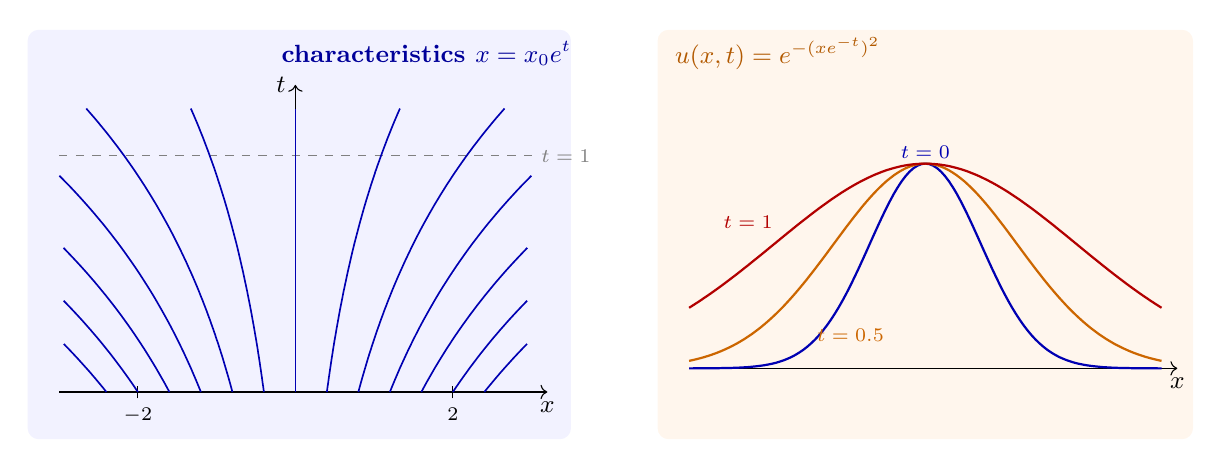
\begin{tikzpicture}[x=1cm,y=1cm]
\fill[blue!5,rounded corners=4pt] (-0.4,-0.6) rectangle (6.5,4.6);
\draw[->] (0,0) -- (6.2,0) node[below,font=\small] {$x$};
\draw[->] (3,0) -- (3,3.9) node[left,font=\small] {$t$};
\foreach \v/\x in {-2/1, 2/5} \draw (\x,-0.08) -- (\x,0.08) node[below,font=\scriptsize] at (\x,-0.08) {$\v$};
\draw[dashed,gray] (0,3) -- (6,3) node[right,font=\scriptsize] {$t = 1$};
\draw[blue!70!black,line width=0.6pt] plot coordinates {(0.600,0.000) (0.551,0.061) (0.500,0.122) (0.449,0.183) (0.397,0.244) (0.343,0.305) (0.288,0.366) (0.233,0.427) (0.176,0.488) (0.118,0.549) (0.059,0.610)};
\draw[blue!70!black,line width=0.6pt] plot coordinates {(1.000,0.000) (0.959,0.061) (0.917,0.122) (0.874,0.183) (0.830,0.244) (0.786,0.305) (0.740,0.366) (0.694,0.427) (0.647,0.488) (0.598,0.549) (0.549,0.610) (0.499,0.671) (0.447,0.732) (0.395,0.793) (0.341,0.854) (0.287,0.915) (0.231,0.976) (0.174,1.037) (0.116,1.098) (0.057,1.159)};
\draw[blue!70!black,line width=0.6pt] plot coordinates {(1.400,0.000) (1.367,0.061) (1.334,0.122) (1.299,0.183) (1.264,0.244) (1.229,0.305) (1.192,0.366) (1.155,0.427) (1.117,0.488) (1.079,0.549) (1.039,0.610) (0.999,0.671) (0.958,0.732) (0.916,0.793) (0.873,0.854) (0.829,0.915) (0.785,0.976) (0.739,1.037) (0.693,1.098) (0.645,1.159) (0.597,1.220) (0.547,1.281) (0.497,1.342) (0.446,1.403) (0.393,1.464) (0.340,1.525) (0.285,1.586) (0.229,1.647) (0.172,1.708) (0.114,1.769) (0.055,1.831)};
\draw[blue!70!black,line width=0.6pt] plot coordinates {(1.800,0.000) (1.775,0.061) (1.750,0.122) (1.724,0.183) (1.698,0.244) (1.672,0.305) (1.644,0.366) (1.616,0.427) (1.588,0.488) (1.559,0.549) (1.529,0.610) (1.499,0.671) (1.468,0.732) (1.437,0.793) (1.405,0.854) (1.372,0.915) (1.338,0.976) (1.304,1.037) (1.269,1.098) (1.234,1.159) (1.198,1.220) (1.161,1.281) (1.123,1.342) (1.084,1.403) (1.045,1.464) (1.005,1.525) (0.964,1.586) (0.922,1.647) (0.879,1.708) (0.836,1.769) (0.791,1.831) (0.746,1.892) (0.699,1.953) (0.652,2.014) (0.604,2.075) (0.555,2.136) (0.504,2.197) (0.453,2.258) (0.401,2.319) (0.347,2.380) (0.293,2.441) (0.237,2.502) (0.181,2.563) (0.123,2.624) (0.063,2.685) (0.003,2.746)};
\draw[blue!70!black,line width=0.6pt] plot coordinates {(2.200,0.000) (2.184,0.061) (2.167,0.122) (2.150,0.183) (2.132,0.244) (2.114,0.305) (2.096,0.366) (2.078,0.427) (2.059,0.488) (2.039,0.549) (2.020,0.610) (1.999,0.671) (1.979,0.732) (1.958,0.793) (1.936,0.854) (1.915,0.915) (1.892,0.976) (1.870,1.037) (1.846,1.098) (1.823,1.159) (1.798,1.220) (1.774,1.281) (1.749,1.342) (1.723,1.403) (1.697,1.464) (1.670,1.525) (1.642,1.586) (1.615,1.647) (1.586,1.708) (1.557,1.769) (1.527,1.831) (1.497,1.892) (1.466,1.953) (1.435,2.014) (1.403,2.075) (1.370,2.136) (1.336,2.197) (1.302,2.258) (1.267,2.319) (1.232,2.380) (1.195,2.441) (1.158,2.502) (1.120,2.563) (1.082,2.624) (1.042,2.685) (1.002,2.746) (0.961,2.807) (0.919,2.868) (0.876,2.929) (0.833,2.990) (0.788,3.051) (0.743,3.112) (0.696,3.173) (0.649,3.234) (0.601,3.295) (0.551,3.356) (0.501,3.417) (0.450,3.478) (0.397,3.539) (0.344,3.600)};
\draw[blue!70!black,line width=0.6pt] plot coordinates {(2.600,0.000) (2.592,0.061) (2.583,0.122) (2.575,0.183) (2.566,0.244) (2.557,0.305) (2.548,0.366) (2.539,0.427) (2.529,0.488) (2.520,0.549) (2.510,0.610) (2.500,0.671) (2.489,0.732) (2.479,0.793) (2.468,0.854) (2.457,0.915) (2.446,0.976) (2.435,1.037) (2.423,1.098) (2.411,1.159) (2.399,1.220) (2.387,1.281) (2.374,1.342) (2.361,1.403) (2.348,1.464) (2.335,1.525) (2.321,1.586) (2.307,1.647) (2.293,1.708) (2.279,1.769) (2.264,1.831) (2.249,1.892) (2.233,1.953) (2.217,2.014) (2.201,2.075) (2.185,2.136) (2.168,2.197) (2.151,2.258) (2.134,2.319) (2.116,2.380) (2.098,2.441) (2.079,2.502) (2.060,2.563) (2.041,2.624) (2.021,2.685) (2.001,2.746) (1.981,2.807) (1.960,2.868) (1.938,2.929) (1.916,2.990) (1.894,3.051) (1.871,3.112) (1.848,3.173) (1.825,3.234) (1.800,3.295) (1.776,3.356) (1.751,3.417) (1.725,3.478) (1.699,3.539) (1.672,3.600)};
\draw[blue!70!black,line width=0.6pt] plot coordinates {(3.000,0.000) (3.000,0.061) (3.000,0.122) (3.000,0.183) (3.000,0.244) (3.000,0.305) (3.000,0.366) (3.000,0.427) (3.000,0.488) (3.000,0.549) (3.000,0.610) (3.000,0.671) (3.000,0.732) (3.000,0.793) (3.000,0.854) (3.000,0.915) (3.000,0.976) (3.000,1.037) (3.000,1.098) (3.000,1.159) (3.000,1.220) (3.000,1.281) (3.000,1.342) (3.000,1.403) (3.000,1.464) (3.000,1.525) (3.000,1.586) (3.000,1.647) (3.000,1.708) (3.000,1.769) (3.000,1.831) (3.000,1.892) (3.000,1.953) (3.000,2.014) (3.000,2.075) (3.000,2.136) (3.000,2.197) (3.000,2.258) (3.000,2.319) (3.000,2.380) (3.000,2.441) (3.000,2.502) (3.000,2.563) (3.000,2.624) (3.000,2.685) (3.000,2.746) (3.000,2.807) (3.000,2.868) (3.000,2.929) (3.000,2.990) (3.000,3.051) (3.000,3.112) (3.000,3.173) (3.000,3.234) (3.000,3.295) (3.000,3.356) (3.000,3.417) (3.000,3.478) (3.000,3.539) (3.000,3.600)};
\draw[blue!70!black,line width=0.6pt] plot coordinates {(3.400,0.000) (3.408,0.061) (3.417,0.122) (3.425,0.183) (3.434,0.244) (3.443,0.305) (3.452,0.366) (3.461,0.427) (3.471,0.488) (3.480,0.549) (3.490,0.610) (3.500,0.671) (3.511,0.732) (3.521,0.793) (3.532,0.854) (3.543,0.915) (3.554,0.976) (3.565,1.037) (3.577,1.098) (3.589,1.159) (3.601,1.220) (3.613,1.281) (3.626,1.342) (3.639,1.403) (3.652,1.464) (3.665,1.525) (3.679,1.586) (3.693,1.647) (3.707,1.708) (3.721,1.769) (3.736,1.831) (3.751,1.892) (3.767,1.953) (3.783,2.014) (3.799,2.075) (3.815,2.136) (3.832,2.197) (3.849,2.258) (3.866,2.319) (3.884,2.380) (3.902,2.441) (3.921,2.502) (3.940,2.563) (3.959,2.624) (3.979,2.685) (3.999,2.746) (4.019,2.807) (4.040,2.868) (4.062,2.929) (4.084,2.990) (4.106,3.051) (4.129,3.112) (4.152,3.173) (4.175,3.234) (4.200,3.295) (4.224,3.356) (4.249,3.417) (4.275,3.478) (4.301,3.539) (4.328,3.600)};
\draw[blue!70!black,line width=0.6pt] plot coordinates {(3.800,0.000) (3.816,0.061) (3.833,0.122) (3.850,0.183) (3.868,0.244) (3.886,0.305) (3.904,0.366) (3.922,0.427) (3.941,0.488) (3.961,0.549) (3.980,0.610) (4.001,0.671) (4.021,0.732) (4.042,0.793) (4.064,0.854) (4.085,0.915) (4.108,0.976) (4.130,1.037) (4.154,1.098) (4.177,1.159) (4.202,1.220) (4.226,1.281) (4.251,1.342) (4.277,1.403) (4.303,1.464) (4.330,1.525) (4.358,1.586) (4.385,1.647) (4.414,1.708) (4.443,1.769) (4.473,1.831) (4.503,1.892) (4.534,1.953) (4.565,2.014) (4.597,2.075) (4.630,2.136) (4.664,2.197) (4.698,2.258) (4.733,2.319) (4.768,2.380) (4.805,2.441) (4.842,2.502) (4.880,2.563) (4.918,2.624) (4.958,2.685) (4.998,2.746) (5.039,2.807) (5.081,2.868) (5.124,2.929) (5.167,2.990) (5.212,3.051) (5.257,3.112) (5.304,3.173) (5.351,3.234) (5.399,3.295) (5.449,3.356) (5.499,3.417) (5.550,3.478) (5.603,3.539) (5.656,3.600)};
\draw[blue!70!black,line width=0.6pt] plot coordinates {(4.200,0.000) (4.225,0.061) (4.250,0.122) (4.276,0.183) (4.302,0.244) (4.328,0.305) (4.356,0.366) (4.384,0.427) (4.412,0.488) (4.441,0.549) (4.471,0.610) (4.501,0.671) (4.532,0.732) (4.563,0.793) (4.595,0.854) (4.628,0.915) (4.662,0.976) (4.696,1.037) (4.731,1.098) (4.766,1.159) (4.802,1.220) (4.839,1.281) (4.877,1.342) (4.916,1.403) (4.955,1.464) (4.995,1.525) (5.036,1.586) (5.078,1.647) (5.121,1.708) (5.164,1.769) (5.209,1.831) (5.254,1.892) (5.301,1.953) (5.348,2.014) (5.396,2.075) (5.445,2.136) (5.496,2.197) (5.547,2.258) (5.599,2.319) (5.653,2.380) (5.707,2.441) (5.763,2.502) (5.819,2.563) (5.877,2.624) (5.937,2.685) (5.997,2.746)};
\draw[blue!70!black,line width=0.6pt] plot coordinates {(4.600,0.000) (4.633,0.061) (4.666,0.122) (4.701,0.183) (4.736,0.244) (4.771,0.305) (4.808,0.366) (4.845,0.427) (4.883,0.488) (4.921,0.549) (4.961,0.610) (5.001,0.671) (5.042,0.732) (5.084,0.793) (5.127,0.854) (5.171,0.915) (5.215,0.976) (5.261,1.037) (5.307,1.098) (5.355,1.159) (5.403,1.220) (5.453,1.281) (5.503,1.342) (5.554,1.403) (5.607,1.464) (5.660,1.525) (5.715,1.586) (5.771,1.647) (5.828,1.708) (5.886,1.769) (5.945,1.831)};
\draw[blue!70!black,line width=0.6pt] plot coordinates {(5.000,0.000) (5.041,0.061) (5.083,0.122) (5.126,0.183) (5.170,0.244) (5.214,0.305) (5.260,0.366) (5.306,0.427) (5.353,0.488) (5.402,0.549) (5.451,0.610) (5.501,0.671) (5.553,0.732) (5.605,0.793) (5.659,0.854) (5.713,0.915) (5.769,0.976) (5.826,1.037) (5.884,1.098) (5.943,1.159)};
\draw[blue!70!black,line width=0.6pt] plot coordinates {(5.400,0.000) (5.449,0.061) (5.500,0.122) (5.551,0.183) (5.603,0.244) (5.657,0.305) (5.712,0.366) (5.767,0.427) (5.824,0.488) (5.882,0.549) (5.941,0.610)};
\node[font=\small\bfseries,blue!60!black,anchor=west] at (2.7,4.3) {characteristics $x = x_0e^t$};
\fill[orange!7,rounded corners=4pt] (7.6,-0.6) rectangle (14.4,4.6);
\draw[->] (8,0.3) -- (14.2,0.3) node[below,font=\small] {$x$};
\draw[blue!70!black,thick] plot coordinates {(8.000,0.300) (8.050,0.300) (8.100,0.301) (8.150,0.301) (8.200,0.301) (8.250,0.301) (8.300,0.302) (8.350,0.302) (8.400,0.303) (8.450,0.304) (8.500,0.305) (8.550,0.306) (8.600,0.308) (8.650,0.310) (8.700,0.313) (8.750,0.316) (8.800,0.321) (8.850,0.326) (8.900,0.332) (8.950,0.339) (9.000,0.348) (9.050,0.358) (9.100,0.370) (9.150,0.385) (9.200,0.402) (9.250,0.422) (9.300,0.444) (9.350,0.471) (9.400,0.501) (9.450,0.535) (9.500,0.574) (9.550,0.618) (9.600,0.666) (9.650,0.720) (9.700,0.780) (9.750,0.845) (9.800,0.916) (9.850,0.993) (9.900,1.075) (9.950,1.163) (10.000,1.256) (10.050,1.354) (10.100,1.457) (10.150,1.562) (10.200,1.671) (10.250,1.781) (10.300,1.893) (10.350,2.004) (10.400,2.114) (10.450,2.221) (10.500,2.325) (10.550,2.423) (10.600,2.516) (10.650,2.600) (10.700,2.676) (10.750,2.742) (10.800,2.798) (10.850,2.842) (10.900,2.874) (10.950,2.894) (11.000,2.900) (11.050,2.894) (11.100,2.874) (11.150,2.842) (11.200,2.798) (11.250,2.742) (11.300,2.676) (11.350,2.600) (11.400,2.516) (11.450,2.423) (11.500,2.325) (11.550,2.221) (11.600,2.114) (11.650,2.004) (11.700,1.893) (11.750,1.781) (11.800,1.671) (11.850,1.562) (11.900,1.457) (11.950,1.354) (12.000,1.256) (12.050,1.163) (12.100,1.075) (12.150,0.993) (12.200,0.916) (12.250,0.845) (12.300,0.780) (12.350,0.720) (12.400,0.666) (12.450,0.618) (12.500,0.574) (12.550,0.535) (12.600,0.501) (12.650,0.471) (12.700,0.444) (12.750,0.422) (12.800,0.402) (12.850,0.385) (12.900,0.370) (12.950,0.358) (13.000,0.348) (13.050,0.339) (13.100,0.332) (13.150,0.326) (13.200,0.321) (13.250,0.316) (13.300,0.313) (13.350,0.310) (13.400,0.308) (13.450,0.306) (13.500,0.305) (13.550,0.304) (13.600,0.303) (13.650,0.302) (13.700,0.302) (13.750,0.301) (13.800,0.301) (13.850,0.301) (13.900,0.301) (13.950,0.300) (14.000,0.300)};
\draw[orange!80!black,thick] plot coordinates {(8.000,0.395) (8.050,0.406) (8.100,0.418) (8.150,0.431) (8.200,0.445) (8.250,0.461) (8.300,0.478) (8.350,0.496) (8.400,0.516) (8.450,0.538) (8.500,0.561) (8.550,0.586) (8.600,0.612) (8.650,0.641) (8.700,0.671) (8.750,0.704) (8.800,0.738) (8.850,0.775) (8.900,0.813) (8.950,0.854) (9.000,0.897) (9.050,0.942) (9.100,0.989) (9.150,1.038) (9.200,1.089) (9.250,1.143) (9.300,1.198) (9.350,1.255) (9.400,1.314) (9.450,1.374) (9.500,1.436) (9.550,1.500) (9.600,1.564) (9.650,1.630) (9.700,1.696) (9.750,1.763) (9.800,1.831) (9.850,1.898) (9.900,1.966) (9.950,2.033) (10.000,2.100) (10.050,2.165) (10.100,2.230) (10.150,2.293) (10.200,2.355) (10.250,2.414) (10.300,2.471) (10.350,2.526) (10.400,2.577) (10.450,2.626) (10.500,2.672) (10.550,2.713) (10.600,2.751) (10.650,2.785) (10.700,2.815) (10.750,2.841) (10.800,2.862) (10.850,2.879) (10.900,2.890) (10.950,2.898) (11.000,2.900) (11.050,2.898) (11.100,2.890) (11.150,2.879) (11.200,2.862) (11.250,2.841) (11.300,2.815) (11.350,2.785) (11.400,2.751) (11.450,2.713) (11.500,2.672) (11.550,2.626) (11.600,2.577) (11.650,2.526) (11.700,2.471) (11.750,2.414) (11.800,2.355) (11.850,2.293) (11.900,2.230) (11.950,2.165) (12.000,2.100) (12.050,2.033) (12.100,1.966) (12.150,1.898) (12.200,1.831) (12.250,1.763) (12.300,1.696) (12.350,1.630) (12.400,1.564) (12.450,1.500) (12.500,1.436) (12.550,1.374) (12.600,1.314) (12.650,1.255) (12.700,1.198) (12.750,1.143) (12.800,1.089) (12.850,1.038) (12.900,0.989) (12.950,0.942) (13.000,0.897) (13.050,0.854) (13.100,0.813) (13.150,0.775) (13.200,0.738) (13.250,0.704) (13.300,0.671) (13.350,0.641) (13.400,0.612) (13.450,0.586) (13.500,0.561) (13.550,0.538) (13.600,0.516) (13.650,0.496) (13.700,0.478) (13.750,0.461) (13.800,0.445) (13.850,0.431) (13.900,0.418) (13.950,0.406) (14.000,0.395)};
\draw[red!70!black,thick] plot coordinates {(8.000,1.069) (8.050,1.101) (8.100,1.133) (8.150,1.166) (8.200,1.200) (8.250,1.234) (8.300,1.269) (8.350,1.305) (8.400,1.341) (8.450,1.378) (8.500,1.416) (8.550,1.454) (8.600,1.492) (8.650,1.531) (8.700,1.571) (8.750,1.610) (8.800,1.651) (8.850,1.691) (8.900,1.731) (8.950,1.772) (9.000,1.813) (9.050,1.854) (9.100,1.895) (9.150,1.936) (9.200,1.977) (9.250,2.018) (9.300,2.058) (9.350,2.099) (9.400,2.139) (9.450,2.178) (9.500,2.217) (9.550,2.256) (9.600,2.294) (9.650,2.332) (9.700,2.368) (9.750,2.404) (9.800,2.440) (9.850,2.474) (9.900,2.507) (9.950,2.540) (10.000,2.571) (10.050,2.601) (10.100,2.630) (10.150,2.658) (10.200,2.684) (10.250,2.709) (10.300,2.733) (10.350,2.756) (10.400,2.776) (10.450,2.796) (10.500,2.814) (10.550,2.830) (10.600,2.844) (10.650,2.857) (10.700,2.869) (10.750,2.878) (10.800,2.886) (10.850,2.892) (10.900,2.896) (10.950,2.899) (11.000,2.900) (11.050,2.899) (11.100,2.896) (11.150,2.892) (11.200,2.886) (11.250,2.878) (11.300,2.869) (11.350,2.857) (11.400,2.844) (11.450,2.830) (11.500,2.814) (11.550,2.796) (11.600,2.776) (11.650,2.756) (11.700,2.733) (11.750,2.709) (11.800,2.684) (11.850,2.658) (11.900,2.630) (11.950,2.601) (12.000,2.571) (12.050,2.540) (12.100,2.507) (12.150,2.474) (12.200,2.440) (12.250,2.404) (12.300,2.368) (12.350,2.332) (12.400,2.294) (12.450,2.256) (12.500,2.217) (12.550,2.178) (12.600,2.139) (12.650,2.099) (12.700,2.058) (12.750,2.018) (12.800,1.977) (12.850,1.936) (12.900,1.895) (12.950,1.854) (13.000,1.813) (13.050,1.772) (13.100,1.731) (13.150,1.691) (13.200,1.651) (13.250,1.610) (13.300,1.571) (13.350,1.531) (13.400,1.492) (13.450,1.454) (13.500,1.416) (13.550,1.378) (13.600,1.341) (13.650,1.305) (13.700,1.269) (13.750,1.234) (13.800,1.200) (13.850,1.166) (13.900,1.133) (13.950,1.101) (14.000,1.069)};
\node[font=\small\bfseries,orange!70!black,anchor=west] at (7.7,4.3) {$u(x, t) = e^{-(xe^{-t})^2}$};
\node[font=\scriptsize,blue!70!black] at (11,3.05) {$t = 0$};
\node[font=\scriptsize,orange!80!black] at (10.05,0.72) {$t = 0.5$};
\node[font=\scriptsize,red!70!black] at (8.75,2.15) {$t = 1$};
\end{tikzpicture}
\caption{The equation $u_t + xu_x = 0$. Left: the characteristics in the $(x, t)$ plane fan out from the origin. Right: since $u$ is constant along each one, the initial Gaussian is stretched horizontally
by the factor $e^t$; its height is unchanged.}
\label{fig:characteristics}
\end{figure}

There is an important distinction between the \textbf{advective} form $u_t + c(x)u_x = 0$ and the \textbf{conservative} form $u_t + (c(x)u)_x = 0$. The second is the law of conservation of a quantity of density $u$ and flux $cu$:
integrating over an interval $[\alpha, \beta]$,
\[
\frac{d}{dt}\int_\alpha^\beta u\,dx = c(\alpha)u(\alpha, t) - c(\beta)u(\beta, t) ,
\]
the rate of change of the amount in the interval equals the inflow minus the outflow. Expanded, it is $u_t + cu_x = -c'u$, which has the same characteristics but a source term: where the flow
converges ($c' < 0$) the density rises. Conservation laws, linear and non-linear, are the subject of the next section.

\subsection{An application: age-structured populations}
\label{ssec:mckendrick}

Let $u(a, t)$ be the density of individuals of age $a$ at time $t$, with death rate $\mu(a)$ and births $B(t)$ at age $0$. Individuals age at rate $1$, so in a short time $h$ those of age $a$ at time $t$ become
those of age $a + h$ at time $t + h$, depleted by deaths: $u(a + h, t + h) = u(a, t)(1 - \mu(a)h) + o(h)$. Dividing by $h$ gives the \textbf{McKendrick--von Foerster equation}
\[
u_t + u_a = -\mu(a)u, \qquad u(0, t) = B(t), \qquad u(a, 0) = u_0(a) .
\]
The characteristics are the lines $a - t = \text{const}$, the life-lines of cohorts, and along each, $du/ds = -\mu u$. Writing $M(a) = \int_0^a\mu$, the solution is
\[
u(a, t) = \begin{cases} u_0(a - t)\,e^{-(M(a) - M(a - t))}, & a \geq t \quad\text{(alive at time } 0),\\ B(t - a)\,e^{-M(a)}, & a < t \quad\text{(born after time } 0). \end{cases}
\]
The two families of characteristics come from the two parts of the boundary of the quadrant $a, t \geq 0$: the initial line $t = 0$ and the birth line $a = 0$. With constant births $B$, after a time
longer than the oldest age the density is the stable age distribution $Be^{-M(a)}$, the \textbf{survival curve} times the birth rate; this is the life table of demography. When births depend on the
population, $B(t) = \int_0^\infty\beta(a)u(a, t)\,da$ with fertility $\beta$, the problem becomes a renewal equation, and the population grows or declines exponentially at a rate fixed by Lotka's equation.

\subsection{Characteristics in software}
\label{ssec:software1}

The panels use Python with SymPy, NumPy and SciPy, as in the companion ODE course, showing commands as typed at the prompt with their output, and MATLAB or Octave equivalents.

\begin{software}[Symbolic solution with \texttt{pdsolve}]
\label{sw:pdsolve}
SymPy solves linear first-order equations with constant coefficients by the method of characteristics, and can verify a proposed general solution:
{\small\begin{verbatim}
>>> import sympy as sp
>>> x, y = sp.symbols('x y'); u = sp.Function('u')
>>> sp.pdsolve(2 * u(x, y).diff(x) + 3 * u(x, y).diff(y), u(x, y))
Eq(u(x, y), F(3*x - 2*y))
>>> sp.pdsolve(u(x, y).diff(x) + u(x, y).diff(y) + u(x, y) - x, u(x, y))
Eq(u(x, y), x + F(x - y)*exp(-x/2 - y/2) - 1)
>>> f = sp.Function('f'); cand = x**2 * f(y / x)       # x u_x + y u_y = 2u
>>> sp.simplify(x * cand.diff(x) + y * cand.diff(y) - 2 * cand)
0
\end{verbatim}}
\textbf{Reading the output.} For $2u_x + 3u_y = 0$ the characteristics are the lines $3x - 2y = \text{const}$, and the solution is an arbitrary function $F$ of $3x - 2y$. For $u_x + u_y + u = x$, the solution is a particular solution $x - 1$
plus an arbitrary function of the characteristic variable $x - y$ times the decaying factor $e^{-(x + y)/2}$. The last line confirms Example~\ref{ex:homogeneousfn}: $x^2F(y/x)$ satisfies $xu_x + yu_y = 2u$ for every $F$.

\textbf{MATLAB/Octave:} the Symbolic Math Toolbox has no general first-order PDE solver; the characteristic ODEs are solved with \texttt{dsolve}.
\end{software}

\begin{software}[Tracing characteristics numerically]
\label{sw:traceback}
For variable speed, the solution at $(x, t)$ is the initial value at the foot of the characteristic through it, found by integrating $dx/d\tau = -c(x)$ backwards from $x$ for time $t$. For $u_t + xu_x = 0$ with
$u(x, 0) = e^{-x^2}$, compared with the exact $f(xe^{-t})$ of Example~\ref{ex:stretch}:
{\small\begin{verbatim}
>>> import numpy as np
>>> from scipy.integrate import solve_ivp
>>> c = lambda x: x                        # u_t + x u_x = 0
>>> f0 = lambda x: np.exp(-x**2)           # u(x, 0)
>>> def u_char(xq, t):                     # follow the characteristic back
...     s = solve_ivp(lambda tau, X: [-c(X[0])], (0, t), [xq], rtol=1e-11)
...     return f0(s.y[0, -1])
...
>>> t = 1.0
>>> for xq in (0.5, 1.5, 3.0):
...     print(xq, round(u_char(xq, t), 6), round(f0(xq * np.exp(-t)), 6))
...
0.5 0.966732 0.966732
1.5 0.737489 0.737489
3.0 0.295816 0.295816
\end{verbatim}}
\textbf{Reading the output.} The numerical and exact values agree to six decimals at all three points. The same code works for any speed $c(x)$, including those for which the characteristics have no
closed form. This is the basis of semi-Lagrangian numerical methods in weather prediction, which follow characteristics back from the grid points at each time step.

\textbf{MATLAB/Octave:} \texttt{[tt, X] = ode45(@(tau, X) -X, [0 1], xq); exp(-X(end)\^{}2)}.
\end{software}

\begin{software}[An age-structured population]
\label{sw:agestructure}
With constant births $B = 100$ a year, death rate $\mu(a) = 0.02 + 0.001a$, and a uniform initial profile of $60$ at every age, the density at four ages after $0$, $20$ and $60$ years, from the characteristic
solution of Section~\ref{ssec:mckendrick}:
{\small\begin{verbatim}
>>> B = 100.0                              # births per year, constant
>>> H = lambda a: 0.02 * a + 0.0005 * a**2  # integral of mu = 0.02 + 0.001a
>>> u0 = lambda a: 60.0                    # uniform initial age profile
>>> def density(a, t):                     # u_t + u_a = -mu(a) u
...     if a >= t:
...         return u0(a - t) * np.exp(-(H(a) - H(a - t)))   # alive at time 0
...     return B * np.exp(-H(a))                     # born after time 0
...
>>> ages = (0, 20, 40, 80)
>>> for t in (0, 20, 60):
...     print(t, [round(density(a, t), 2) for a in ages])
...
0 [60.0, 60.0, 60.0, 60.0]
20 [100.0, 32.93, 22.07, 9.92]
60 [100.0, 54.88, 20.19, 0.9]
>>> [round(B * np.exp(-H(a)), 2) for a in ages]   # the steady state
[100.0, 54.88, 20.19, 0.82]
\end{verbatim}}
\textbf{Reading the output.} At ages below $t$ the density already equals the stable distribution $Be^{-M(a)}$ (the last line), because those individuals were born after time $0$. After $20$ years only age $0$ is
on the birth branch among the ages shown; the age-$20$ cohort was aged $0$ at time $0$, so it comes from the initial population, $60e^{-M(20)} = 32.93$ rather than $54.88$. After $60$ years the ages $0$, $20$
and $40$ all match the stable values. The age-$80$ density, $0.90$ after $60$ years, still comes from the initial population, and differs from the stable value $0.82$; it will
reach it only when the last of the initial cohort has died. Information about the initial state travels along characteristics and leaves the system through the old ages.

\textbf{MATLAB/Octave:} the same piecewise formula as a function handle.
\end{software}

\subsection{Practice Problems}

\begin{problem}
Solve $u_t + 3u_x = 0$, $u(x, 0) = \sin x$, and $u_t + 3u_x = t$, $u(x, 0) = \sin x$.
\end{problem}

\begin{solution}
By Theorem~\ref{thm:transport}, $u = \sin(x - 3t)$ for the first. For the second, $u = \sin(x - 3t) + \int_0^ts\,ds = \sin(x - 3t) + \frac{t^2}{2}$: the source raises $u$ along each characteristic.
\end{solution}

\begin{problem}
Find the general solution of $yu_x - xu_y = 0$, and solve it with $u(x, 0) = x^2$ for $x > 0$.
\end{problem}

\begin{solution}
The characteristics solve $x' = y$, $y' = -x$: circles $x^2 + y^2 = \text{const}$. So $u = F(x^2 + y^2)$, radially symmetric. With $u(x, 0) = F(x^2) = x^2$, $F(r) = r$ and $u = x^2 + y^2$. The data line $y = 0$, $x > 0$ crosses each
circle exactly once, as Theorem~\ref{thm:cauchy1} requires; data on the whole line $y = 0$ would have to be even in $x$, or no solution would exist.
\end{solution}

\begin{problem}
Solve $u_x + 2u_y = -u$ with $u(x, 0) = f(x)$.
\end{problem}

\begin{solution}
The characteristics are $x = x_0 + s$, $y = 2s$, starting from $(x_0, 0)$, along which $du/ds = -u$, so $u = f(x_0)e^{-s}$. Inverting, $s = y/2$ and $x_0 = x - y/2$, so $u(x, y) = f(x - y/2)e^{-y/2}$.
\end{solution}

\begin{problem}
Show that the Cauchy problem $u_x + u_y = 0$ with data on the line $y = x$ has no solution if $u = x$ there, and infinitely many if $u = 1$ there.
\end{problem}

\begin{solution}
The line $y = x$ is a characteristic (direction $(1, 1)$). Along it $u$ must be constant. Data $u = x$ are not constant, so there is no solution. Data $u = 1$ are constant, and $u = 1 + G(x - y)$ is a solution for every $C^1$
function $G$ with $G(0) = 0$: infinitely many.
\end{solution}

\begin{problem}
Solve $u_t + (xu)_x = 0$, $u(x, 0) = f(x)$, and show that $\int_{-\infty}^\infty u\,dx$ is constant in time, unlike for $u_t + xu_x = 0$.
\end{problem}

\begin{solution}
Expanded, $u_t + xu_x = -u$. Along $x = x_0e^t$, $du/dt = -u$, so $u = f(x_0)e^{-t} = f(xe^{-t})e^{-t}$. Then $\int u\,dx = e^{-t}\int f(xe^{-t})\,dx = e^{-t}e^t\int f(y)\,dy = \int f$, constant: the conservative form preserves the total amount, spreading it out while
lowering its peak. For $u_t + xu_x = 0$, $u = f(xe^{-t})$ and $\int u = e^t\int f$, which grows.
\end{solution}

\begin{problem}
In the McKendrick--von Foerster model with constant death rate $\mu$ and constant births $B$, find the stable age distribution and the total population, and show that the mean age is $1/\mu$.
\end{problem}

\begin{solution}
$M(a) = \mu a$, so the stable distribution is $Be^{-\mu a}$, with total $\int_0^\infty Be^{-\mu a}\,da = B/\mu$. The mean age is $\int_0^\infty aBe^{-\mu a}\,da/(B/\mu) = (B/\mu^2)/(B/\mu) = 1/\mu$, which is also the life expectancy at birth: with a death rate of $2\%$ a year,
the mean age is $50$ years.
\end{solution}

%======================================================================
\section{Non-linear Conservation Laws and Shocks}
\label{sec:shocks}

For a linear first-order equation the characteristics are fixed in advance, by the coefficients. For a quasilinear equation such as $u_t + uu_x = 0$ the
speed of each characteristic depends on the solution itself, so faster parts of a wave can catch up with slower parts, characteristics cross, and a
smooth solution ceases to exist after a finite time: the wave \textbf{breaks}. What happens next cannot be described by a classical solution at all.
The resolution, weak solutions with discontinuities called shocks, selected by an entropy condition, is one of the central ideas of the subject, and it
governs gas dynamics, traffic flow, river floods and blast waves. This section develops it for scalar equations in one space dimension.

\subsection{Quasilinear equations and breaking}
\label{ssec:quasilinear}

\begin{defn}
A scalar \textbf{conservation law} is $u_t + f(u)_x = 0$, with \textbf{flux} $f$, or for smooth solutions $u_t + a(u)u_x = 0$ with $a = f'$. The basic example is the inviscid \textbf{Burgers equation},
$f(u) = \frac12u^2$, $a(u) = u$.
\end{defn}

By the method of Section~\ref{sec:characteristics}, along a curve with $dx/dt = a(u)$ the solution satisfies $du/dt = u_t + a(u)u_x = 0$, so $u$ is constant on the curve, and therefore so is its speed $a(u)$: the
characteristics are \emph{straight lines}, $x = x_0 + a(u_0(x_0))t$, each carrying its initial value.

\begin{thm}
\label{thm:breaking}
Let $u_0$ be $C^1$ and bounded with bounded derivative, and $a$ be $C^1$. The initial value problem $u_t + a(u)u_x = 0$, $u(x, 0) = u_0(x)$, has a $C^1$ solution, given implicitly by
\[
u = u_0\bigl(x - a(u)t\bigr),
\]
for $0 \leq t < t_b$, where
\[
t_b = -\frac{1}{\inf_x\,\frac{d}{dx}a(u_0(x))}
\]
($t_b = \infty$ if $a(u_0)$ is non-decreasing). If $t_b < \infty$, the derivative $u_x$ becomes unbounded as $t \to t_b$, and no $C^1$ solution exists beyond $t_b$.
\end{thm}

\begin{proof}
Write $\sigma(x_0) = a(u_0(x_0))$, the speed of the characteristic from $x_0$. The map $x_0 \mapsto X(x_0, t) = x_0 + \sigma(x_0)t$ has derivative $1 + \sigma'(x_0)t$, which is positive for all $x_0$ exactly when $t < t_b$; it is then
strictly increasing and, since $\sigma$ is bounded, onto $\mathbb R$. So each $(x, t)$ lies on exactly one characteristic, with foot $x_0(x, t)$, and $u(x, t) = u_0(x_0(x, t))$ is $C^1$ by the inverse function theorem. Differentiating,
\[
u_x = \frac{u_0'(x_0)}{1 + \sigma'(x_0)t} ,
\]
and along the characteristic where $\sigma'$ attains (or approaches) its infimum, the denominator tends to $0$ as $t \to t_b$ while the numerator does not (since $\sigma' = a'(u_0)u_0'$), so $u_x \to \infty$. At $t_b$ two
characteristics carrying different values meet, and $u$ would have to take both values at one point.
\end{proof}

For Burgers' equation, $\sigma = u_0$ and $t_b = -1/\min u_0'$: the wave breaks first where it is steepest on its front. For $u_0 = e^{-x^2}$, $\min u_0' = -\sqrt2e^{-1/2}$ at $x = 1/\sqrt2$, and $t_b = e^{1/2}/\sqrt2 = 1.166$
(Figure~\ref{fig:breaking}). The top of the hump travels faster than its foot and overtakes it, exactly as an ocean wave steepens and breaks on a beach.

\begin{figure}[H]
\centering
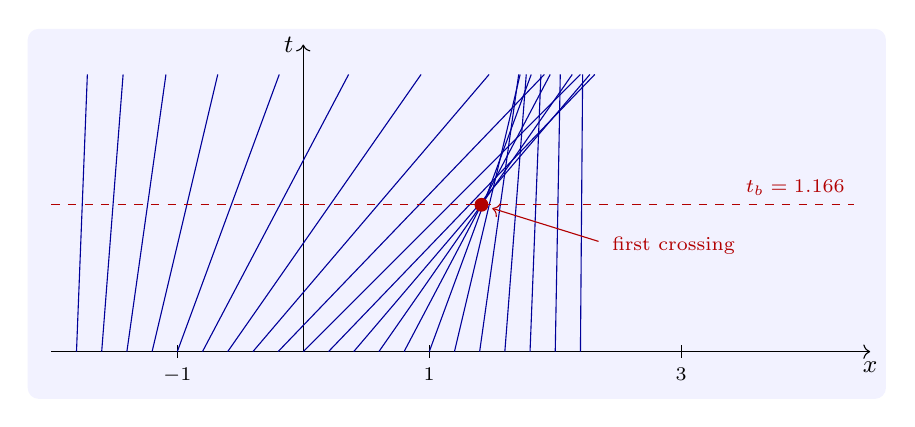
\begin{tikzpicture}[x=1cm,y=1cm]
\fill[blue!5,rounded corners=4pt] (-0.3,-0.6) rectangle (10.6,4.1);
\draw[->] (0,0) -- (10.4,0) node[below,font=\small] {$x$};
\draw[->] (3.2,0) -- (3.2,3.9) node[left,font=\small] {$t$};
\foreach \v/\x in {-1/1.6, 1/4.8, 3/8.0} \draw (\x,-0.08) -- (\x,0.08) node[below,font=\scriptsize] at (\x,-0.08) {$\v$};
\draw[blue!60!black] (0.320,0.000) -- (0.458,3.520);
\draw[blue!60!black] (0.640,0.000) -- (0.912,3.520);
\draw[blue!60!black] (0.960,0.000) -- (1.456,3.520);
\draw[blue!60!black] (1.280,0.000) -- (2.114,3.520);
\draw[blue!60!black] (1.600,0.000) -- (2.895,3.520);
\draw[blue!60!black] (1.920,0.000) -- (3.776,3.520);
\draw[blue!60!black] (2.240,0.000) -- (4.696,3.520);
\draw[blue!60!black] (2.560,0.000) -- (5.560,3.520);
\draw[blue!60!black] (2.880,0.000) -- (6.262,3.520);
\draw[blue!60!black] (3.200,0.000) -- (6.720,3.520);
\draw[blue!60!black] (3.520,0.000) -- (6.902,3.520);
\draw[blue!60!black] (3.840,0.000) -- (6.840,3.520);
\draw[blue!60!black] (4.160,0.000) -- (6.616,3.520);
\draw[blue!60!black] (4.480,0.000) -- (6.336,3.520);
\draw[blue!60!black] (4.800,0.000) -- (6.095,3.520);
\draw[blue!60!black] (5.120,0.000) -- (5.954,3.520);
\draw[blue!60!black] (5.440,0.000) -- (5.936,3.520);
\draw[blue!60!black] (5.760,0.000) -- (6.032,3.520);
\draw[blue!60!black] (6.080,0.000) -- (6.218,3.520);
\draw[blue!60!black] (6.400,0.000) -- (6.464,3.520);
\draw[blue!60!black] (6.720,0.000) -- (6.748,3.520);
\draw[red!70!black,dashed] (0,1.865) -- (10.2,1.865) node[above left,font=\scriptsize] {$t_b = 1.166$};
\fill[red!70!black] (5.463,1.865) circle (2.5pt);
\node[font=\scriptsize,red!70!black,anchor=west,fill=blue!5] at (7.0,1.35) {first crossing};
\draw[red!70!black,->] (6.95,1.4) -- (5.6,1.82);
\end{tikzpicture}
\caption{Characteristics of Burgers' equation $u_t + uu_x = 0$ with $u_0(x) = e^{-x^2}$. Each line has slope $dx/dt = u_0(x_0)$, so the characteristics from the top of the hump are fastest. Those from the front of the hump
converge, and the first pair crosses at $t_b = 1.166$, where the wave breaks.}
\label{fig:breaking}
\end{figure}

\subsection{Weak solutions and the Rankine--Hugoniot condition}
\label{ssec:weak}

After breaking, the conservation law still makes sense in its integral form: for every interval $[\alpha, \beta]$,
\[
\frac{d}{dt}\int_\alpha^\beta u\,dx = f\bigl(u(\alpha, t)\bigr) - f\bigl(u(\beta, t)\bigr) ,
\]
which does not require derivatives of $u$. Equivalently, $u$ is a \textbf{weak solution} if for every smooth test function $\phi$ with compact support in $\mathbb R \times [0, \infty)$,
\[
\int_0^\infty\!\!\int_{-\infty}^\infty\bigl(u\phi_t + f(u)\phi_x\bigr)\,dx\,dt + \int_{-\infty}^\infty u_0(x)\phi(x, 0)\,dx = 0 ,
\]
obtained by multiplying the equation by $\phi$ and integrating by parts. A classical solution is a weak solution, and a weak solution that is $C^1$ is classical. Weak solutions may have jumps.

\begin{thm}[Rankine--Hugoniot]
\label{thm:rh}
Let $u$ be a weak solution that is $C^1$ on either side of a curve $x = s(t)$, with limits $u_l$ and $u_r$ on the left and right. Then the speed of the discontinuity satisfies
\[
s'(t) = \frac{f(u_r) - f(u_l)}{u_r - u_l} = \frac{[f]}{[u]} .
\]
For Burgers' equation, $s' = \frac12(u_l + u_r)$.
\end{thm}

\begin{proof}
Take $\alpha < s(t) < \beta$ with $[\alpha, \beta]$ small. Splitting the integral at the shock and differentiating,
\[
\frac{d}{dt}\Bigl(\int_\alpha^{s(t)}u\,dx + \int_{s(t)}^\beta u\,dx\Bigr) = \int_\alpha^{s}u_t\,dx + \int_{s}^\beta u_t\,dx + s'u_l - s'u_r .
\]
On each side $u_t = -f(u)_x$, so the integrals equal $f(u(\alpha)) - f(u_l) + f(u_r) - f(u(\beta))$. Comparing with the integral form of the law, $f(u(\alpha)) - f(u(\beta))$, gives $s'(u_l - u_r) = f(u_l) - f(u_r)$.
\end{proof}

The condition says that the amount of $u$ swept up as the shock moves is supplied by the difference of the fluxes on its two sides. It applies to any conservation law, and is the jump
condition across a shock wave in a gas.

\subsection{The Riemann problem and the entropy condition}
\label{ssec:riemann}

The \textbf{Riemann problem} has piecewise constant data, $u_0 = u_l$ for $x < 0$ and $u_r$ for $x > 0$. For Burgers' equation there are two cases.
\begin{enumerate}[label=(\roman*)]
\item If $u_l > u_r$, the characteristics from the left are faster and run into those from the right, and the solution is a \textbf{shock} moving at the Rankine--Hugoniot speed $s = \frac12(u_l + u_r)$:
$u = u_l$ for $x < st$, $u = u_r$ for $x > st$.
\item If $u_l < u_r$, the characteristics diverge, leaving a wedge $u_lt < x < u_rt$ that no characteristic from $t = 0$ reaches. The solution there is the \textbf{rarefaction fan} $u = x/t$, the only self-similar continuous
solution, which joins $u_l$ to $u_r$ (Figure~\ref{fig:riemann}).
\end{enumerate}
In case (ii) the discontinuous function $u = u_l$ for $x < st$, $u = u_r$ for $x > st$, with $s = \frac12(u_l + u_r)$, is also a weak solution: weak solutions are not unique. The non-physical one has characteristics
coming \emph{out} of the shock, which would create information from nothing. The \textbf{Lax entropy condition} rules it out:
\[
a(u_l) > s > a(u_r),
\]
that is, characteristics must run \emph{into} a shock from both sides. With this condition, and more generally with Kru\v{z}kov's entropy inequalities, the Cauchy problem for a scalar conservation law
has a unique weak solution. The entropy solution is also the limit as $\nu \to 0$ of the viscous Burgers equation $u_t + uu_x = \nu u_{xx}$, whose shock is a smooth transition of width of order $\nu$: the physically correct solution is the one that small
diffusion selects.

\begin{figure}[H]
\centering
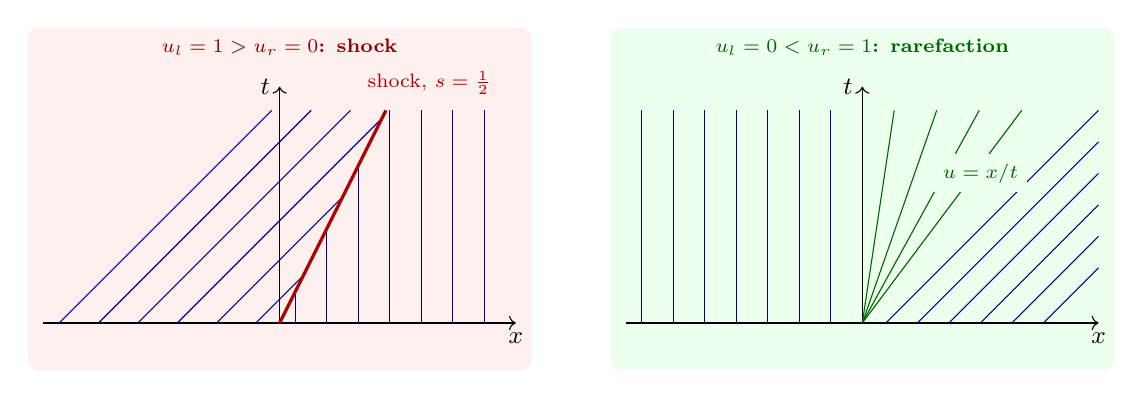
\begin{tikzpicture}[x=1cm,y=1cm]
\begin{scope}
\fill[red!6,rounded corners=4pt] (-3.2,-0.6) rectangle (3.2,3.75);
\draw[->] (-3,0) -- (3,0) node[below,font=\small] {$x$}; \draw[->] (0,0) -- (0,3) node[left,font=\small] {$t$};
\draw[blue!60!black] (-2.80,0) -- (-0.100,2.700);
\draw[blue!60!black] (-2.30,0) -- (0.400,2.700);
\draw[blue!60!black] (-1.80,0) -- (0.900,2.700);
\draw[blue!60!black] (-1.30,0) -- (1.300,2.600);
\draw[blue!60!black] (-0.80,0) -- (0.800,1.600);
\draw[blue!60!black] (-0.30,0) -- (0.300,0.600);
\draw[blue!60!black] (0.20,0) -- (0.20,0.400);
\draw[blue!60!black] (0.60,0) -- (0.60,1.200);
\draw[blue!60!black] (1.00,0) -- (1.00,2.000);
\draw[blue!60!black] (1.40,0) -- (1.40,2.700);
\draw[blue!60!black] (1.80,0) -- (1.80,2.700);
\draw[blue!60!black] (2.20,0) -- (2.20,2.700);
\draw[blue!60!black] (2.60,0) -- (2.60,2.700);
\draw[red!70!black,very thick] (0,0) -- (1.35,2.7);
\node[font=\scriptsize,red!70!black] at (1.9,3.05) {shock, $s = \frac12$};
\node[font=\scriptsize\bfseries,red!60!black] at (0,3.5) {$u_l = 1 > u_r = 0$: shock};
\end{scope}
\begin{scope}[shift={(7.4,0)}]
\fill[green!7,rounded corners=4pt] (-3.2,-0.6) rectangle (3.2,3.75);
\draw[->] (-3,0) -- (3,0) node[below,font=\small] {$x$}; \draw[->] (0,0) -- (0,3) node[left,font=\small] {$t$};
\foreach \x in {-2.8,-2.4,...,-0.3} \draw[blue!60!black] (\x,0) -- (\x,2.7);
\draw[blue!60!black] (0.30,0) -- (3.000,2.700);
\draw[blue!60!black] (0.70,0) -- (3.000,2.300);
\draw[blue!60!black] (1.10,0) -- (3.000,1.900);
\draw[blue!60!black] (1.50,0) -- (3.000,1.500);
\draw[blue!60!black] (1.90,0) -- (3.000,1.100);
\draw[blue!60!black] (2.30,0) -- (3.000,0.700);
\foreach \k in {0.15,0.35,...,0.95} \draw[green!40!black] (0,0) -- ({\k*2.7},2.7);
\node[font=\scriptsize\bfseries,green!40!black] at (0,3.5) {$u_l = 0 < u_r = 1$: rarefaction};
\node[font=\scriptsize,green!40!black,fill=green!7] at (1.5,1.9) {$u = x/t$};
\end{scope}
\end{tikzpicture}
\caption{Riemann problems for Burgers' equation in the $(x, t)$ plane. Left: the characteristics from both sides run into a shock moving at the Rankine--Hugoniot speed $\frac12(u_l + u_r)$. Right: the characteristics diverge,
and the gap is filled by the fan of characteristics $x = ct$, $0 \leq c \leq 1$, from the origin, on which $u = x/t$.}
\label{fig:riemann}
\end{figure}

\subsection{Traffic flow}
\label{ssec:traffic}

Lighthill and Whitham (1955) and Richards (1956) modelled road traffic by the density $\rho(x, t)$ of cars, in cars per kilometre, with flux $q = \rho v(\rho)$. The speed falls from $v_{\max}$ on an empty road to $0$ at the
jam density $\rho_{\max}$; the simplest choice is $v = v_{\max}(1 - \rho/\rho_{\max})$, giving the conservation law
\[
\rho_t + q(\rho)_x = 0, \qquad q(\rho) = v_{\max}\rho\Bigl(1 - \frac{\rho}{\rho_{\max}}\Bigr) .
\]
The flux is greatest, $q_{\max} = \frac14v_{\max}\rho_{\max}$, at $\rho_c = \frac12\rho_{\max}$: the capacity of the road. The characteristic speed $q'(\rho) = v_{\max}(1 - 2\rho/\rho_{\max})$ is the speed at which \emph{disturbances} travel, which is less than
the speed of the cars $v(\rho)$, and negative in dense traffic: a disturbance in heavy traffic travels backwards, against the flow, as every driver who has braked for no visible reason knows.

At a red light, cars arriving at density $\rho_l$ meet stopped cars at $\rho_r = \rho_{\max}$. Since $q'(\rho_l) > q'(\rho_{\max})$, this is a shock, the back of the queue, and by Rankine--Hugoniot it moves at speed
\[
s = \frac{q(\rho_{\max}) - q(\rho_l)}{\rho_{\max} - \rho_l} = -v_{\max}\frac{\rho_l}{\rho_{\max}} ,
\]
backwards. When the light turns green, the jam at $\rho_{\max}$ on the left faces an empty road on the right, and the solution is a rarefaction fan in which the density thins out continuously:
the front cars accelerate away while the cars further back are still waiting for the fan to reach them.

\subsection{Conservation laws in software}
\label{ssec:software2}

\begin{software}[The breaking time]
\label{sw:breaking}
For Burgers' equation with $u_0 = e^{-x^2}$, the breaking time from Theorem~\ref{thm:breaking}, and a direct check that the characteristic map $x_0 \mapsto x_0 + u_0(x_0)t$ stops being monotone:
{\small\begin{verbatim}
>>> import numpy as np
>>> u0 = lambda x: np.exp(-x**2)           # u_t + u u_x = 0
>>> du0 = lambda x: -2 * x * np.exp(-x**2)
>>> xs = np.linspace(-3, 3, 600001)
>>> tb = -1 / du0(xs).min(); tb, 1 / (np.sqrt(2) * np.exp(-0.5))
(1.1658219908227196, 1.165821990798562)
>>> X = lambda x0, t: x0 + u0(x0) * t      # straight characteristics
>>> for t in (1.0, tb, 1.5):
...     print(round(t, 4), bool(np.all(np.diff(X(xs, t)) > 0)))   # ordered?
...
1.0 True
1.1658 False
1.5 False
\end{verbatim}}
\textbf{Reading the output.} The minimum of $u_0'$ on a fine grid gives $t_b = 1.16582$, agreeing with $e^{1/2}/\sqrt2$ to ten digits. At $t = 1$ the characteristic positions are still in order, so the solution is
single-valued; at $t_b$ and after, they are not, and the classical solution has ceased to exist.

\textbf{MATLAB/Octave:} \texttt{-1/min(gradient(exp(-x.\^{}2), x))}.
\end{software}

\begin{software}[Conservative and non-conservative schemes]
\label{sw:godunov}
Godunov's method updates cell averages using the exact flux of the Riemann problem at each cell interface. It is compared with a naive upwind discretisation of $u_t + uu_x = 0$, which is consistent with
the equation for smooth solutions but is not in conservation form. Riemann data $u_l = 2$, $u_r = 0$ until $T = 2$; then the reverse data:
{\small\begin{verbatim}
>>> def godunov(ul, ur):                   # Riemann flux, f(u) = u^2/2
...     shock = np.where(ul + ur > 0, ul**2, ur**2) / 2
...     fan = np.where(ul > 0, ul**2 / 2, np.where(ur < 0, ur**2 / 2, 0.0))
...     return np.where(ul > ur, shock, fan)
...
>>> def solve(uL, uR, conservative, N=800, L=8.0, T=2.0):
...     dx = L / N; x = -L / 2 + dx * (np.arange(N) + 0.5)
...     u = np.where(x < 0, uL, uR); dt = 0.4 * dx / max(abs(uL), abs(uR))
...     for _ in range(int(round(T / dt))):
...         if conservative:
...             F = godunov(u[:-1], u[1:])
...             u[1:-1] -= dt / dx * (F[1:] - F[:-1])
...         else:                          # upwind on u u_x: not conservative
...             u[1:] -= dt / dx * u[1:] * (u[1:] - u[:-1])
...     return x, u
...
>>> for cons in (True, False):             # uL = 2, uR = 0, until T = 2
...     x, u = solve(2.0, 0.0, cons)
...     print(cons, round(x[np.argmax(u < 1.0)], 3))   # where u drops
...
True 2.005
False 0.005
>>> x, u = solve(0.0, 2.0, True)           # the reverse: a rarefaction fan
>>> [round(float(np.interp(q, x, u)), 3) for q in (-1.0, 1.0, 2.0, 3.0, 5.0)]
[0.0, 0.512, 1.007, 1.498, 2.0]
\end{verbatim}}
\textbf{Reading the output.} The exact shock speed is $\frac12(2 + 0) = 1$, so at $T = 2$ the shock is at $x = 2$. Godunov's method places it at $2.005$, within one cell. The non-conservative scheme leaves it at the origin, $0.005$: it
converges, but to the wrong weak solution, because it does not respect the integral form of the law on which the Rankine--Hugoniot condition rests. This is the Lax--Wendroff theorem in negative form:
conservative schemes that converge, converge to weak solutions; non-conservative ones need not. For the reverse data, Godunov's method produces the fan $u = x/t$: at $x = 1, 2, 3$ the values $0.51$, $1.01$, $1.50$
against the exact $0.5$, $1$, $1.5$.

\textbf{MATLAB/Octave:} the same vectorised update in a loop.
\end{software}

\begin{software}[A red light]
\label{sw:traffic}
For a road with $v_{\max} = 100$\,km/h and jam density $150$ cars/km, traffic at $50$ cars/km meets a queue at a red light:
{\small\begin{verbatim}
>>> vmax, rmax = 100.0, 150.0              # km/h, cars per km (jammed)
>>> flux = lambda r: r * vmax * (1 - r / rmax)
>>> speed = lambda r: vmax * (1 - 2 * r / rmax)       # characteristic speed
>>> rL, rR = 50.0, 150.0                   # queue at a red light ahead
>>> (flux(rR) - flux(rL)) / (rR - rL), speed(rL), speed(rR)
(-33.333333333333336, 33.333333333333336, -100.0)
>>> rc = rmax / 2; rc, flux(rc)            # density of maximum flow, capacity
(75.0, 3750.0)
\end{verbatim}}
\textbf{Reading the output.} The back of the queue moves backwards at $33.3$\,km/h, equal to $v_{\max}\rho_l/\rho_{\max}$. The entropy condition holds: the characteristic speeds on the two sides, $+33.3$ and $-100$\,km/h, both run into the shock. The capacity of
the road is $3750$ cars an hour, at the critical density $75$ cars/km, where cars travel at $50$\,km/h.

\textbf{MATLAB/Octave:} \texttt{q = @(r) r*100.*(1 - r/150); (q(150) - q(50))/(150 - 50)}.
\end{software}

\subsection{Practice Problems}

\begin{problem}
Find the breaking time for Burgers' equation with $u_0(x) = \sin x$, and where the first shock forms.
\end{problem}

\begin{solution}
$\min u_0' = \min\cos x = -1$, at $x = \pi$, so $t_b = 1$. The characteristic from $x_0 = \pi$ has speed $\sin\pi = 0$, so the shock forms at $x = \pi$, $t = 1$, and stays there by symmetry: $u$ is odd about $\pi$, so $u_l = -u_r$ and
$s = 0$.
\end{solution}

\begin{problem}
Solve Burgers' equation with $u_0 = 1$ for $x < 0$, $u_0 = 1 - x$ for $0 \leq x \leq 1$, $u_0 = 0$ for $x > 1$, up to breaking, and continue the solution after.
\end{problem}

\begin{solution}
Characteristics from $x_0 \in [0, 1]$ have speed $1 - x_0$ and are $x = x_0 + (1 - x_0)t$; all of them meet at $x = 1$, $t = 1$, so $t_b = 1$. For $t < 1$, in the ramp, $x = x_0 + (1 - x_0)t$ gives $x_0 = (x - t)/(1 - t)$ and
$u = 1 - x_0 = (1 - x)/(1 - t)$ for $t \leq x \leq 1$; $u = 1$ for $x < t$; $u = 0$ for $x > 1$. At $t = 1$ a shock forms at $x = 1$ joining $u_l = 1$ to $u_r = 0$; it moves at speed $\frac12$, so $x = 1 + \frac12(t - 1)$ for $t \geq 1$.
\end{solution}

\begin{problem}
Show that for $u_l < u_r$ the fan $u = x/t$ satisfies Burgers' equation, and that the discontinuous weak solution with speed $\frac12(u_l + u_r)$ violates the entropy condition.
\end{problem}

\begin{solution}
$u_t + uu_x = -\frac{x}{t^2} + \frac xt\cdot\frac1t = 0$. For the discontinuous solution, $a(u_l) = u_l < \frac12(u_l + u_r) < u_r = a(u_r)$, so $a(u_l) < s$ and $s < a(u_r)$, the reverse of the Lax condition: characteristics leave the shock on both sides.
\end{solution}

\begin{problem}
For the traffic model of Section~\ref{ssec:traffic}, show that the shock at the back of a queue has speed $-v_{\max}\rho_l/\rho_{\max}$, and find how long a queue grows behind a light that is red for $60$ seconds, with
$v_{\max} = 100$\,km/h, $\rho_{\max} = 150$ and $\rho_l = 50$ cars/km.
\end{problem}

\begin{solution}
$q(\rho_{\max}) = 0$, so
\[
s = -\frac{q(\rho_l)}{\rho_{\max} - \rho_l} = -\frac{v_{\max}\rho_l(1 - \rho_l/\rho_{\max})}{\rho_{\max}(1 - \rho_l/\rho_{\max})} = -v_{\max}\frac{\rho_l}{\rho_{\max}} .
\]
Here $s = -33.3$\,km/h, so after one minute the back of the queue is $33.3/60 = 0.556$\,km behind the light, and the queue holds $0.556 \times 150 = 83.3$ cars. As a check by conservation: $0.556 \times 50 = 27.8$ cars were already on that stretch when the light turned red, and $q(\rho_l)/60 = 3333/60 = 55.6$ more arrived during the minute, $83.3$ in all.
\end{solution}

\begin{problem}
Find the shock speed for the conservation law $u_t + (u^3)_x = 0$ with $u_l = 1$, $u_r = 0$, and check the entropy condition.
\end{problem}

\begin{solution}
$s = (0 - 1)/(0 - 1) = 1$. With $a(u) = 3u^2$, $a(u_l) = 3 > 1 > 0 = a(u_r)$: the Lax condition holds, and the shock is admissible.
\end{solution}

%======================================================================
\section{Classification of Second-order Equations}
\label{sec:classification}

The three great equations of mathematical physics, the wave, heat and Laplace equations, behave in completely different ways. Waves travel at finite speed and keep their sharp edges, heat spreads instantly and smooths everything, and harmonic functions are
determined everywhere by their boundary values. This section shows that every linear second-order equation in two variables is, locally, like one of the three, according to the sign of a single discriminant, and that the type decides which data make
a problem well posed.

\subsection{The discriminant and its invariance}
\label{ssec:discriminant}

Consider the linear equation
\begin{equation}
\label{eq:secondorder}
a u_{xx} + 2b u_{xy} + c u_{yy} + d u_x + e u_y + f u = g ,
\end{equation}
with coefficients depending on $(x, y)$. Its \textbf{principal part} is $a u_{xx} + 2b u_{xy} + c u_{yy}$, with symmetric matrix $M = \begin{pmatrix} a & b \\ b & c \end{pmatrix}$.

\begin{defn}
At a point, equation \eqref{eq:secondorder} is \textbf{hyperbolic} if $b^2 - ac > 0$, \textbf{parabolic} if $b^2 - ac = 0$ (with $M \neq 0$), and \textbf{elliptic} if $b^2 - ac < 0$.
\end{defn}

The wave equation $u_{tt} - u_{xx} = 0$ ($a = -1$, $c = 1$ in the variables $(x, t)$, $b^2 - ac = 1$) is hyperbolic; the heat equation $u_t - u_{xx} = 0$ ($a = -1$, $b = c = 0$) is parabolic; Laplace's equation $u_{xx} + u_{yy} = 0$ ($b^2 - ac = -1$) is elliptic.
The names come from the conics $ax^2 + 2bxy + cy^2 = 1$.

\begin{thm}
\label{thm:typeinvariant}
Under a smooth change of variables $\xi = \xi(x, y)$, $\eta = \eta(x, y)$ with Jacobian $J = \xi_x\eta_y - \xi_y\eta_x \neq 0$, equation \eqref{eq:secondorder} becomes $Au_{\xi\xi} + 2Bu_{\xi\eta} + Cu_{\eta\eta} + (\text{lower order}) = g$, where
\begin{align*}
A &= a\xi_x^2 + 2b\xi_x\xi_y + c\xi_y^2, \\
B &= a\xi_x\eta_x + b(\xi_x\eta_y + \xi_y\eta_x) + c\xi_y\eta_y, \\
C &= a\eta_x^2 + 2b\eta_x\eta_y + c\eta_y^2 ,
\end{align*}
and $B^2 - AC = J^2(b^2 - ac)$. In particular the type is unchanged by any change of variables.
\end{thm}

\begin{proof}
By the chain rule $u_x = u_\xi\xi_x + u_\eta\eta_x$, and differentiating again, the second derivatives of $u$ in the new variables appear only through products of first derivatives of $\xi$ and $\eta$; the second derivatives of $\xi$ and $\eta$ multiply $u_\xi$ and $u_\eta$, and go into the lower-order terms. Collecting
terms gives $A$, $B$, $C$ above. In matrix form this says
\[
\begin{pmatrix} A & B \\ B & C \end{pmatrix} = D M D^{\mathsf T}, \qquad D = \begin{pmatrix} \xi_x & \xi_y \\ \eta_x & \eta_y \end{pmatrix} ,
\]
and taking determinants, $AC - B^2 = (\det D)^2(ac - b^2) = J^2(ac - b^2)$.
\end{proof}

In $n$ variables, the principal part $\sum_{i,j}a_{ij}u_{x_ix_j}$ has a symmetric matrix $(a_{ij})$, and a linear change of variables replaces it by $DAD^{\mathsf T}$; by Sylvester's law of inertia the numbers of positive, negative and zero eigenvalues are invariant. The equation is \textbf{elliptic} if all eigenvalues
have one sign, \textbf{hyperbolic} if all but one have one sign and the last the other, and \textbf{parabolic} if one is zero and the rest have one sign. The wave equation $u_{tt} = c^2\Delta u$ has eigenvalues $1, -c^2, \ldots, -c^2$, and is hyperbolic; the heat and Laplace equations in
$n$ dimensions are parabolic and elliptic. Other sign patterns (\emph{ultra-hyperbolic}) can occur when $n \geq 4$, but have no comparable role in physics.

\subsection{Characteristics and canonical forms}
\label{ssec:canonical}

The coefficient $A$ vanishes when $\xi$ satisfies the \textbf{characteristic equation}
\[
a\varphi_x^2 + 2b\varphi_x\varphi_y + c\varphi_y^2 = 0 .
\]
A level curve $\varphi(x, y) = \text{const}$ of such a function is a \textbf{characteristic curve}. Along it $dy/dx = -\varphi_x/\varphi_y$, and the characteristic equation becomes an ordinary differential equation for the slope $m = dy/dx$:
\[
a m^2 - 2b m + c = 0, \qquad m = \frac{b \pm \sqrt{b^2 - ac}}{a} .
\]
So a hyperbolic equation has two real families of characteristics, a parabolic equation one, and an elliptic equation none. As in Section~\ref{sec:characteristics}, characteristics are the curves on which Cauchy data cannot be prescribed freely, and across which
solutions may have discontinuities in their second derivatives; in the hyperbolic case they are the paths of waves.

\begin{thm}[Canonical forms]
\label{thm:canonical}
Near any point, equation \eqref{eq:secondorder} can be transformed into
\begin{enumerate}[label=(\roman*)]
\item $u_{\xi\eta} + (\text{lower order}) = g$ if it is hyperbolic, taking $\xi$ and $\eta$ constant on the two families of characteristics; equivalently $u_{\alpha\alpha} - u_{\beta\beta} + \ldots$ with $\alpha = \xi + \eta$, $\beta = \xi - \eta$;
\item $u_{\eta\eta} + (\text{lower order}) = g$ if it is parabolic, taking $\xi$ constant on the characteristics and $\eta$ any function with $J \neq 0$;
\item $u_{\alpha\alpha} + u_{\beta\beta} + (\text{lower order}) = g$ if it is elliptic, with $\alpha$, $\beta$ the real and imaginary parts of a complex solution of the characteristic equation (assuming analytic coefficients; in general one solves a Beltrami equation).
\end{enumerate}
\end{thm}

\begin{proof}
(i) With $\xi$ and $\eta$ characteristic, $A = C = 0$, and $B \neq 0$ since $B^2 = J^2(b^2 - ac) > 0$; divide by $2B$. (ii) With $\xi$ characteristic, $A = 0$, so $B^2 = AC + J^2(b^2 - ac) = 0$, and $C \neq 0$ since otherwise the principal part would vanish; divide by $C$.
(iii) If $\varphi = \alpha + i\beta$ satisfies the characteristic equation, then $Q(\varphi) = a\varphi_x^2 + 2b\varphi_x\varphi_y + c\varphi_y^2 = 0$, and separating real and imaginary parts,
\[
Q(\alpha) - Q(\beta) = 0, \qquad a\alpha_x\beta_x + b(\alpha_x\beta_y + \alpha_y\beta_x) + c\alpha_y\beta_y = 0 ,
\]
which say that the coefficients of $u_{\alpha\alpha}$ and $u_{\beta\beta}$ are equal and that of $u_{\alpha\beta}$ is zero.
\end{proof}

\begin{exa}
\label{ex:canonical}
For $u_{xx} + 4u_{xy} + 3u_{yy} = 0$, $b^2 - ac = 4 - 3 = 1$: hyperbolic. The slopes solve $m^2 - 4m + 3 = 0$, so $m = 1$ and $3$, and $\xi = y - x$, $\eta = y - 3x$ are constant on the characteristics. Then $A = C = 0$ and
$B = 1\cdot 3 + 2(-1 - 3) + 3 = -2$, so the equation is $-4u_{\xi\eta} = 0$, and integrating twice,
\[
u = F(y - x) + G(y - 3x)
\]
for arbitrary $F$ and $G$: the sum of two waves, one on each family of characteristics.
\end{exa}

\begin{exa}[The Tricomi equation]
\label{ex:tricomi}
The type can change from point to point. For $yu_{xx} + u_{yy} = 0$, $b^2 - ac = -y$: the equation is elliptic in the upper half-plane, hyperbolic in the lower, and parabolic on the axis. In $y < 0$ the slopes satisfy $ym^2 + 1 = 0$, so
$dx/dy = \pm\sqrt{-y}$ and the characteristics are the cusped curves
\[
x = x_0 \pm \tfrac23(-y)^{3/2}
\]
(Figure~\ref{fig:tricomi}). Tricomi (1923) studied it as the model of a \emph{mixed-type} problem, and it describes the steady flow of a gas near the speed of sound, which is subsonic (elliptic) on one side of the sonic line and supersonic (hyperbolic) on the other.
\end{exa}

\begin{figure}[H]
\centering
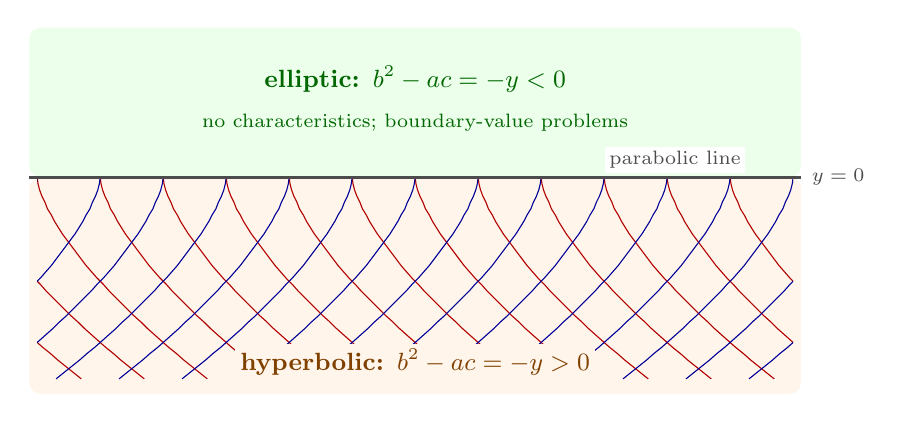
\begin{tikzpicture}[x=1cm,y=1cm]
\fill[green!8,rounded corners=4pt] (-4.9,0) rectangle (4.9,1.9);
\fill[orange!8,rounded corners=4pt] (-4.9,-2.75) rectangle (4.9,0);
\begin{scope}
\clip (-4.8,-2.6) rectangle (4.8,0);
\draw[red!70!black] (-6.40,0.00) -- (-6.39,-0.08) -- (-6.37,-0.16) -- (-6.34,-0.24) -- (-6.30,-0.32) -- (-6.27,-0.40) -- (-6.22,-0.48) -- (-6.18,-0.56) -- (-6.13,-0.64) -- (-6.08,-0.72) -- (-6.02,-0.80) -- (-5.96,-0.88) -- (-5.90,-0.96) -- (-5.84,-1.04) -- (-5.78,-1.12) -- (-5.71,-1.20) -- (-5.64,-1.28) -- (-5.56,-1.36) -- (-5.49,-1.44) -- (-5.41,-1.52) -- (-5.33,-1.60) -- (-5.25,-1.68) -- (-5.17,-1.76) -- (-5.08,-1.84) -- (-5.00,-1.92) -- (-4.91,-2.00) -- (-4.82,-2.08) -- (-4.73,-2.16) -- (-4.63,-2.24) -- (-4.54,-2.32) -- (-4.44,-2.40) -- (-4.34,-2.48) -- (-4.24,-2.56);
\draw[blue!60!black] (-6.40,0.00) -- (-6.41,-0.08) -- (-6.43,-0.16) -- (-6.46,-0.24) -- (-6.50,-0.32) -- (-6.53,-0.40) -- (-6.58,-0.48) -- (-6.62,-0.56) -- (-6.67,-0.64) -- (-6.72,-0.72) -- (-6.78,-0.80) -- (-6.84,-0.88) -- (-6.90,-0.96) -- (-6.96,-1.04) -- (-7.02,-1.12) -- (-7.09,-1.20) -- (-7.16,-1.28) -- (-7.24,-1.36) -- (-7.31,-1.44) -- (-7.39,-1.52) -- (-7.47,-1.60) -- (-7.55,-1.68) -- (-7.63,-1.76) -- (-7.72,-1.84) -- (-7.80,-1.92) -- (-7.89,-2.00) -- (-7.98,-2.08) -- (-8.07,-2.16) -- (-8.17,-2.24) -- (-8.26,-2.32) -- (-8.36,-2.40) -- (-8.46,-2.48) -- (-8.56,-2.56);
\draw[red!70!black] (-5.60,0.00) -- (-5.59,-0.08) -- (-5.57,-0.16) -- (-5.54,-0.24) -- (-5.50,-0.32) -- (-5.47,-0.40) -- (-5.42,-0.48) -- (-5.38,-0.56) -- (-5.33,-0.64) -- (-5.28,-0.72) -- (-5.22,-0.80) -- (-5.16,-0.88) -- (-5.10,-0.96) -- (-5.04,-1.04) -- (-4.98,-1.12) -- (-4.91,-1.20) -- (-4.84,-1.28) -- (-4.76,-1.36) -- (-4.69,-1.44) -- (-4.61,-1.52) -- (-4.53,-1.60) -- (-4.45,-1.68) -- (-4.37,-1.76) -- (-4.28,-1.84) -- (-4.20,-1.92) -- (-4.11,-2.00) -- (-4.02,-2.08) -- (-3.93,-2.16) -- (-3.83,-2.24) -- (-3.74,-2.32) -- (-3.64,-2.40) -- (-3.54,-2.48) -- (-3.44,-2.56);
\draw[blue!60!black] (-5.60,0.00) -- (-5.61,-0.08) -- (-5.63,-0.16) -- (-5.66,-0.24) -- (-5.70,-0.32) -- (-5.73,-0.40) -- (-5.78,-0.48) -- (-5.82,-0.56) -- (-5.87,-0.64) -- (-5.92,-0.72) -- (-5.98,-0.80) -- (-6.04,-0.88) -- (-6.10,-0.96) -- (-6.16,-1.04) -- (-6.22,-1.12) -- (-6.29,-1.20) -- (-6.36,-1.28) -- (-6.44,-1.36) -- (-6.51,-1.44) -- (-6.59,-1.52) -- (-6.67,-1.60) -- (-6.75,-1.68) -- (-6.83,-1.76) -- (-6.92,-1.84) -- (-7.00,-1.92) -- (-7.09,-2.00) -- (-7.18,-2.08) -- (-7.27,-2.16) -- (-7.37,-2.24) -- (-7.46,-2.32) -- (-7.56,-2.40) -- (-7.66,-2.48) -- (-7.76,-2.56);
\draw[red!70!black] (-4.80,0.00) -- (-4.79,-0.08) -- (-4.77,-0.16) -- (-4.74,-0.24) -- (-4.70,-0.32) -- (-4.67,-0.40) -- (-4.62,-0.48) -- (-4.58,-0.56) -- (-4.53,-0.64) -- (-4.48,-0.72) -- (-4.42,-0.80) -- (-4.36,-0.88) -- (-4.30,-0.96) -- (-4.24,-1.04) -- (-4.18,-1.12) -- (-4.11,-1.20) -- (-4.04,-1.28) -- (-3.96,-1.36) -- (-3.89,-1.44) -- (-3.81,-1.52) -- (-3.73,-1.60) -- (-3.65,-1.68) -- (-3.57,-1.76) -- (-3.48,-1.84) -- (-3.40,-1.92) -- (-3.31,-2.00) -- (-3.22,-2.08) -- (-3.13,-2.16) -- (-3.03,-2.24) -- (-2.94,-2.32) -- (-2.84,-2.40) -- (-2.74,-2.48) -- (-2.64,-2.56);
\draw[blue!60!black] (-4.80,0.00) -- (-4.81,-0.08) -- (-4.83,-0.16) -- (-4.86,-0.24) -- (-4.90,-0.32) -- (-4.93,-0.40) -- (-4.98,-0.48) -- (-5.02,-0.56) -- (-5.07,-0.64) -- (-5.12,-0.72) -- (-5.18,-0.80) -- (-5.24,-0.88) -- (-5.30,-0.96) -- (-5.36,-1.04) -- (-5.42,-1.12) -- (-5.49,-1.20) -- (-5.56,-1.28) -- (-5.64,-1.36) -- (-5.71,-1.44) -- (-5.79,-1.52) -- (-5.87,-1.60) -- (-5.95,-1.68) -- (-6.03,-1.76) -- (-6.12,-1.84) -- (-6.20,-1.92) -- (-6.29,-2.00) -- (-6.38,-2.08) -- (-6.47,-2.16) -- (-6.57,-2.24) -- (-6.66,-2.32) -- (-6.76,-2.40) -- (-6.86,-2.48) -- (-6.96,-2.56);
\draw[red!70!black] (-4.00,0.00) -- (-3.99,-0.08) -- (-3.97,-0.16) -- (-3.94,-0.24) -- (-3.90,-0.32) -- (-3.87,-0.40) -- (-3.82,-0.48) -- (-3.78,-0.56) -- (-3.73,-0.64) -- (-3.68,-0.72) -- (-3.62,-0.80) -- (-3.56,-0.88) -- (-3.50,-0.96) -- (-3.44,-1.04) -- (-3.38,-1.12) -- (-3.31,-1.20) -- (-3.24,-1.28) -- (-3.16,-1.36) -- (-3.09,-1.44) -- (-3.01,-1.52) -- (-2.93,-1.60) -- (-2.85,-1.68) -- (-2.77,-1.76) -- (-2.68,-1.84) -- (-2.60,-1.92) -- (-2.51,-2.00) -- (-2.42,-2.08) -- (-2.33,-2.16) -- (-2.23,-2.24) -- (-2.14,-2.32) -- (-2.04,-2.40) -- (-1.94,-2.48) -- (-1.84,-2.56);
\draw[blue!60!black] (-4.00,0.00) -- (-4.01,-0.08) -- (-4.03,-0.16) -- (-4.06,-0.24) -- (-4.10,-0.32) -- (-4.13,-0.40) -- (-4.18,-0.48) -- (-4.22,-0.56) -- (-4.27,-0.64) -- (-4.32,-0.72) -- (-4.38,-0.80) -- (-4.44,-0.88) -- (-4.50,-0.96) -- (-4.56,-1.04) -- (-4.62,-1.12) -- (-4.69,-1.20) -- (-4.76,-1.28) -- (-4.84,-1.36) -- (-4.91,-1.44) -- (-4.99,-1.52) -- (-5.07,-1.60) -- (-5.15,-1.68) -- (-5.23,-1.76) -- (-5.32,-1.84) -- (-5.40,-1.92) -- (-5.49,-2.00) -- (-5.58,-2.08) -- (-5.67,-2.16) -- (-5.77,-2.24) -- (-5.86,-2.32) -- (-5.96,-2.40) -- (-6.06,-2.48) -- (-6.16,-2.56);
\draw[red!70!black] (-3.20,0.00) -- (-3.19,-0.08) -- (-3.17,-0.16) -- (-3.14,-0.24) -- (-3.10,-0.32) -- (-3.07,-0.40) -- (-3.02,-0.48) -- (-2.98,-0.56) -- (-2.93,-0.64) -- (-2.88,-0.72) -- (-2.82,-0.80) -- (-2.76,-0.88) -- (-2.70,-0.96) -- (-2.64,-1.04) -- (-2.58,-1.12) -- (-2.51,-1.20) -- (-2.44,-1.28) -- (-2.36,-1.36) -- (-2.29,-1.44) -- (-2.21,-1.52) -- (-2.13,-1.60) -- (-2.05,-1.68) -- (-1.97,-1.76) -- (-1.88,-1.84) -- (-1.80,-1.92) -- (-1.71,-2.00) -- (-1.62,-2.08) -- (-1.53,-2.16) -- (-1.43,-2.24) -- (-1.34,-2.32) -- (-1.24,-2.40) -- (-1.14,-2.48) -- (-1.04,-2.56);
\draw[blue!60!black] (-3.20,0.00) -- (-3.21,-0.08) -- (-3.23,-0.16) -- (-3.26,-0.24) -- (-3.30,-0.32) -- (-3.33,-0.40) -- (-3.38,-0.48) -- (-3.42,-0.56) -- (-3.47,-0.64) -- (-3.52,-0.72) -- (-3.58,-0.80) -- (-3.64,-0.88) -- (-3.70,-0.96) -- (-3.76,-1.04) -- (-3.82,-1.12) -- (-3.89,-1.20) -- (-3.96,-1.28) -- (-4.04,-1.36) -- (-4.11,-1.44) -- (-4.19,-1.52) -- (-4.27,-1.60) -- (-4.35,-1.68) -- (-4.43,-1.76) -- (-4.52,-1.84) -- (-4.60,-1.92) -- (-4.69,-2.00) -- (-4.78,-2.08) -- (-4.87,-2.16) -- (-4.97,-2.24) -- (-5.06,-2.32) -- (-5.16,-2.40) -- (-5.26,-2.48) -- (-5.36,-2.56);
\draw[red!70!black] (-2.40,0.00) -- (-2.39,-0.08) -- (-2.37,-0.16) -- (-2.34,-0.24) -- (-2.30,-0.32) -- (-2.27,-0.40) -- (-2.22,-0.48) -- (-2.18,-0.56) -- (-2.13,-0.64) -- (-2.08,-0.72) -- (-2.02,-0.80) -- (-1.96,-0.88) -- (-1.90,-0.96) -- (-1.84,-1.04) -- (-1.78,-1.12) -- (-1.71,-1.20) -- (-1.64,-1.28) -- (-1.56,-1.36) -- (-1.49,-1.44) -- (-1.41,-1.52) -- (-1.33,-1.60) -- (-1.25,-1.68) -- (-1.17,-1.76) -- (-1.08,-1.84) -- (-1.00,-1.92) -- (-0.91,-2.00) -- (-0.82,-2.08) -- (-0.73,-2.16) -- (-0.63,-2.24) -- (-0.54,-2.32) -- (-0.44,-2.40) -- (-0.34,-2.48) -- (-0.24,-2.56);
\draw[blue!60!black] (-2.40,0.00) -- (-2.41,-0.08) -- (-2.43,-0.16) -- (-2.46,-0.24) -- (-2.50,-0.32) -- (-2.53,-0.40) -- (-2.58,-0.48) -- (-2.62,-0.56) -- (-2.67,-0.64) -- (-2.72,-0.72) -- (-2.78,-0.80) -- (-2.84,-0.88) -- (-2.90,-0.96) -- (-2.96,-1.04) -- (-3.02,-1.12) -- (-3.09,-1.20) -- (-3.16,-1.28) -- (-3.24,-1.36) -- (-3.31,-1.44) -- (-3.39,-1.52) -- (-3.47,-1.60) -- (-3.55,-1.68) -- (-3.63,-1.76) -- (-3.72,-1.84) -- (-3.80,-1.92) -- (-3.89,-2.00) -- (-3.98,-2.08) -- (-4.07,-2.16) -- (-4.17,-2.24) -- (-4.26,-2.32) -- (-4.36,-2.40) -- (-4.46,-2.48) -- (-4.56,-2.56);
\draw[red!70!black] (-1.60,0.00) -- (-1.59,-0.08) -- (-1.57,-0.16) -- (-1.54,-0.24) -- (-1.50,-0.32) -- (-1.47,-0.40) -- (-1.42,-0.48) -- (-1.38,-0.56) -- (-1.33,-0.64) -- (-1.28,-0.72) -- (-1.22,-0.80) -- (-1.16,-0.88) -- (-1.10,-0.96) -- (-1.04,-1.04) -- (-0.98,-1.12) -- (-0.91,-1.20) -- (-0.84,-1.28) -- (-0.76,-1.36) -- (-0.69,-1.44) -- (-0.61,-1.52) -- (-0.53,-1.60) -- (-0.45,-1.68) -- (-0.37,-1.76) -- (-0.28,-1.84) -- (-0.20,-1.92) -- (-0.11,-2.00) -- (-0.02,-2.08) -- (0.07,-2.16) -- (0.17,-2.24) -- (0.26,-2.32) -- (0.36,-2.40) -- (0.46,-2.48) -- (0.56,-2.56);
\draw[blue!60!black] (-1.60,0.00) -- (-1.61,-0.08) -- (-1.63,-0.16) -- (-1.66,-0.24) -- (-1.70,-0.32) -- (-1.73,-0.40) -- (-1.78,-0.48) -- (-1.82,-0.56) -- (-1.87,-0.64) -- (-1.92,-0.72) -- (-1.98,-0.80) -- (-2.04,-0.88) -- (-2.10,-0.96) -- (-2.16,-1.04) -- (-2.22,-1.12) -- (-2.29,-1.20) -- (-2.36,-1.28) -- (-2.44,-1.36) -- (-2.51,-1.44) -- (-2.59,-1.52) -- (-2.67,-1.60) -- (-2.75,-1.68) -- (-2.83,-1.76) -- (-2.92,-1.84) -- (-3.00,-1.92) -- (-3.09,-2.00) -- (-3.18,-2.08) -- (-3.27,-2.16) -- (-3.37,-2.24) -- (-3.46,-2.32) -- (-3.56,-2.40) -- (-3.66,-2.48) -- (-3.76,-2.56);
\draw[red!70!black] (-0.80,0.00) -- (-0.79,-0.08) -- (-0.77,-0.16) -- (-0.74,-0.24) -- (-0.70,-0.32) -- (-0.67,-0.40) -- (-0.62,-0.48) -- (-0.58,-0.56) -- (-0.53,-0.64) -- (-0.48,-0.72) -- (-0.42,-0.80) -- (-0.36,-0.88) -- (-0.30,-0.96) -- (-0.24,-1.04) -- (-0.18,-1.12) -- (-0.11,-1.20) -- (-0.04,-1.28) -- (0.04,-1.36) -- (0.11,-1.44) -- (0.19,-1.52) -- (0.27,-1.60) -- (0.35,-1.68) -- (0.43,-1.76) -- (0.52,-1.84) -- (0.60,-1.92) -- (0.69,-2.00) -- (0.78,-2.08) -- (0.87,-2.16) -- (0.97,-2.24) -- (1.06,-2.32) -- (1.16,-2.40) -- (1.26,-2.48) -- (1.36,-2.56);
\draw[blue!60!black] (-0.80,0.00) -- (-0.81,-0.08) -- (-0.83,-0.16) -- (-0.86,-0.24) -- (-0.90,-0.32) -- (-0.93,-0.40) -- (-0.98,-0.48) -- (-1.02,-0.56) -- (-1.07,-0.64) -- (-1.12,-0.72) -- (-1.18,-0.80) -- (-1.24,-0.88) -- (-1.30,-0.96) -- (-1.36,-1.04) -- (-1.42,-1.12) -- (-1.49,-1.20) -- (-1.56,-1.28) -- (-1.64,-1.36) -- (-1.71,-1.44) -- (-1.79,-1.52) -- (-1.87,-1.60) -- (-1.95,-1.68) -- (-2.03,-1.76) -- (-2.12,-1.84) -- (-2.20,-1.92) -- (-2.29,-2.00) -- (-2.38,-2.08) -- (-2.47,-2.16) -- (-2.57,-2.24) -- (-2.66,-2.32) -- (-2.76,-2.40) -- (-2.86,-2.48) -- (-2.96,-2.56);
\draw[red!70!black] (0.00,0.00) -- (0.01,-0.08) -- (0.03,-0.16) -- (0.06,-0.24) -- (0.10,-0.32) -- (0.13,-0.40) -- (0.18,-0.48) -- (0.22,-0.56) -- (0.27,-0.64) -- (0.32,-0.72) -- (0.38,-0.80) -- (0.44,-0.88) -- (0.50,-0.96) -- (0.56,-1.04) -- (0.62,-1.12) -- (0.69,-1.20) -- (0.76,-1.28) -- (0.84,-1.36) -- (0.91,-1.44) -- (0.99,-1.52) -- (1.07,-1.60) -- (1.15,-1.68) -- (1.23,-1.76) -- (1.32,-1.84) -- (1.40,-1.92) -- (1.49,-2.00) -- (1.58,-2.08) -- (1.67,-2.16) -- (1.77,-2.24) -- (1.86,-2.32) -- (1.96,-2.40) -- (2.06,-2.48) -- (2.16,-2.56);
\draw[blue!60!black] (0.00,0.00) -- (-0.01,-0.08) -- (-0.03,-0.16) -- (-0.06,-0.24) -- (-0.10,-0.32) -- (-0.13,-0.40) -- (-0.18,-0.48) -- (-0.22,-0.56) -- (-0.27,-0.64) -- (-0.32,-0.72) -- (-0.38,-0.80) -- (-0.44,-0.88) -- (-0.50,-0.96) -- (-0.56,-1.04) -- (-0.62,-1.12) -- (-0.69,-1.20) -- (-0.76,-1.28) -- (-0.84,-1.36) -- (-0.91,-1.44) -- (-0.99,-1.52) -- (-1.07,-1.60) -- (-1.15,-1.68) -- (-1.23,-1.76) -- (-1.32,-1.84) -- (-1.40,-1.92) -- (-1.49,-2.00) -- (-1.58,-2.08) -- (-1.67,-2.16) -- (-1.77,-2.24) -- (-1.86,-2.32) -- (-1.96,-2.40) -- (-2.06,-2.48) -- (-2.16,-2.56);
\draw[red!70!black] (0.80,0.00) -- (0.81,-0.08) -- (0.83,-0.16) -- (0.86,-0.24) -- (0.90,-0.32) -- (0.93,-0.40) -- (0.98,-0.48) -- (1.02,-0.56) -- (1.07,-0.64) -- (1.12,-0.72) -- (1.18,-0.80) -- (1.24,-0.88) -- (1.30,-0.96) -- (1.36,-1.04) -- (1.42,-1.12) -- (1.49,-1.20) -- (1.56,-1.28) -- (1.64,-1.36) -- (1.71,-1.44) -- (1.79,-1.52) -- (1.87,-1.60) -- (1.95,-1.68) -- (2.03,-1.76) -- (2.12,-1.84) -- (2.20,-1.92) -- (2.29,-2.00) -- (2.38,-2.08) -- (2.47,-2.16) -- (2.57,-2.24) -- (2.66,-2.32) -- (2.76,-2.40) -- (2.86,-2.48) -- (2.96,-2.56);
\draw[blue!60!black] (0.80,0.00) -- (0.79,-0.08) -- (0.77,-0.16) -- (0.74,-0.24) -- (0.70,-0.32) -- (0.67,-0.40) -- (0.62,-0.48) -- (0.58,-0.56) -- (0.53,-0.64) -- (0.48,-0.72) -- (0.42,-0.80) -- (0.36,-0.88) -- (0.30,-0.96) -- (0.24,-1.04) -- (0.18,-1.12) -- (0.11,-1.20) -- (0.04,-1.28) -- (-0.04,-1.36) -- (-0.11,-1.44) -- (-0.19,-1.52) -- (-0.27,-1.60) -- (-0.35,-1.68) -- (-0.43,-1.76) -- (-0.52,-1.84) -- (-0.60,-1.92) -- (-0.69,-2.00) -- (-0.78,-2.08) -- (-0.87,-2.16) -- (-0.97,-2.24) -- (-1.06,-2.32) -- (-1.16,-2.40) -- (-1.26,-2.48) -- (-1.36,-2.56);
\draw[red!70!black] (1.60,0.00) -- (1.61,-0.08) -- (1.63,-0.16) -- (1.66,-0.24) -- (1.70,-0.32) -- (1.73,-0.40) -- (1.78,-0.48) -- (1.82,-0.56) -- (1.87,-0.64) -- (1.92,-0.72) -- (1.98,-0.80) -- (2.04,-0.88) -- (2.10,-0.96) -- (2.16,-1.04) -- (2.22,-1.12) -- (2.29,-1.20) -- (2.36,-1.28) -- (2.44,-1.36) -- (2.51,-1.44) -- (2.59,-1.52) -- (2.67,-1.60) -- (2.75,-1.68) -- (2.83,-1.76) -- (2.92,-1.84) -- (3.00,-1.92) -- (3.09,-2.00) -- (3.18,-2.08) -- (3.27,-2.16) -- (3.37,-2.24) -- (3.46,-2.32) -- (3.56,-2.40) -- (3.66,-2.48) -- (3.76,-2.56);
\draw[blue!60!black] (1.60,0.00) -- (1.59,-0.08) -- (1.57,-0.16) -- (1.54,-0.24) -- (1.50,-0.32) -- (1.47,-0.40) -- (1.42,-0.48) -- (1.38,-0.56) -- (1.33,-0.64) -- (1.28,-0.72) -- (1.22,-0.80) -- (1.16,-0.88) -- (1.10,-0.96) -- (1.04,-1.04) -- (0.98,-1.12) -- (0.91,-1.20) -- (0.84,-1.28) -- (0.76,-1.36) -- (0.69,-1.44) -- (0.61,-1.52) -- (0.53,-1.60) -- (0.45,-1.68) -- (0.37,-1.76) -- (0.28,-1.84) -- (0.20,-1.92) -- (0.11,-2.00) -- (0.02,-2.08) -- (-0.07,-2.16) -- (-0.17,-2.24) -- (-0.26,-2.32) -- (-0.36,-2.40) -- (-0.46,-2.48) -- (-0.56,-2.56);
\draw[red!70!black] (2.40,0.00) -- (2.41,-0.08) -- (2.43,-0.16) -- (2.46,-0.24) -- (2.50,-0.32) -- (2.53,-0.40) -- (2.58,-0.48) -- (2.62,-0.56) -- (2.67,-0.64) -- (2.72,-0.72) -- (2.78,-0.80) -- (2.84,-0.88) -- (2.90,-0.96) -- (2.96,-1.04) -- (3.02,-1.12) -- (3.09,-1.20) -- (3.16,-1.28) -- (3.24,-1.36) -- (3.31,-1.44) -- (3.39,-1.52) -- (3.47,-1.60) -- (3.55,-1.68) -- (3.63,-1.76) -- (3.72,-1.84) -- (3.80,-1.92) -- (3.89,-2.00) -- (3.98,-2.08) -- (4.07,-2.16) -- (4.17,-2.24) -- (4.26,-2.32) -- (4.36,-2.40) -- (4.46,-2.48) -- (4.56,-2.56);
\draw[blue!60!black] (2.40,0.00) -- (2.39,-0.08) -- (2.37,-0.16) -- (2.34,-0.24) -- (2.30,-0.32) -- (2.27,-0.40) -- (2.22,-0.48) -- (2.18,-0.56) -- (2.13,-0.64) -- (2.08,-0.72) -- (2.02,-0.80) -- (1.96,-0.88) -- (1.90,-0.96) -- (1.84,-1.04) -- (1.78,-1.12) -- (1.71,-1.20) -- (1.64,-1.28) -- (1.56,-1.36) -- (1.49,-1.44) -- (1.41,-1.52) -- (1.33,-1.60) -- (1.25,-1.68) -- (1.17,-1.76) -- (1.08,-1.84) -- (1.00,-1.92) -- (0.91,-2.00) -- (0.82,-2.08) -- (0.73,-2.16) -- (0.63,-2.24) -- (0.54,-2.32) -- (0.44,-2.40) -- (0.34,-2.48) -- (0.24,-2.56);
\draw[red!70!black] (3.20,0.00) -- (3.21,-0.08) -- (3.23,-0.16) -- (3.26,-0.24) -- (3.30,-0.32) -- (3.33,-0.40) -- (3.38,-0.48) -- (3.42,-0.56) -- (3.47,-0.64) -- (3.52,-0.72) -- (3.58,-0.80) -- (3.64,-0.88) -- (3.70,-0.96) -- (3.76,-1.04) -- (3.82,-1.12) -- (3.89,-1.20) -- (3.96,-1.28) -- (4.04,-1.36) -- (4.11,-1.44) -- (4.19,-1.52) -- (4.27,-1.60) -- (4.35,-1.68) -- (4.43,-1.76) -- (4.52,-1.84) -- (4.60,-1.92) -- (4.69,-2.00) -- (4.78,-2.08) -- (4.87,-2.16) -- (4.97,-2.24) -- (5.06,-2.32) -- (5.16,-2.40) -- (5.26,-2.48) -- (5.36,-2.56);
\draw[blue!60!black] (3.20,0.00) -- (3.19,-0.08) -- (3.17,-0.16) -- (3.14,-0.24) -- (3.10,-0.32) -- (3.07,-0.40) -- (3.02,-0.48) -- (2.98,-0.56) -- (2.93,-0.64) -- (2.88,-0.72) -- (2.82,-0.80) -- (2.76,-0.88) -- (2.70,-0.96) -- (2.64,-1.04) -- (2.58,-1.12) -- (2.51,-1.20) -- (2.44,-1.28) -- (2.36,-1.36) -- (2.29,-1.44) -- (2.21,-1.52) -- (2.13,-1.60) -- (2.05,-1.68) -- (1.97,-1.76) -- (1.88,-1.84) -- (1.80,-1.92) -- (1.71,-2.00) -- (1.62,-2.08) -- (1.53,-2.16) -- (1.43,-2.24) -- (1.34,-2.32) -- (1.24,-2.40) -- (1.14,-2.48) -- (1.04,-2.56);
\draw[red!70!black] (4.00,0.00) -- (4.01,-0.08) -- (4.03,-0.16) -- (4.06,-0.24) -- (4.10,-0.32) -- (4.13,-0.40) -- (4.18,-0.48) -- (4.22,-0.56) -- (4.27,-0.64) -- (4.32,-0.72) -- (4.38,-0.80) -- (4.44,-0.88) -- (4.50,-0.96) -- (4.56,-1.04) -- (4.62,-1.12) -- (4.69,-1.20) -- (4.76,-1.28) -- (4.84,-1.36) -- (4.91,-1.44) -- (4.99,-1.52) -- (5.07,-1.60) -- (5.15,-1.68) -- (5.23,-1.76) -- (5.32,-1.84) -- (5.40,-1.92) -- (5.49,-2.00) -- (5.58,-2.08) -- (5.67,-2.16) -- (5.77,-2.24) -- (5.86,-2.32) -- (5.96,-2.40) -- (6.06,-2.48) -- (6.16,-2.56);
\draw[blue!60!black] (4.00,0.00) -- (3.99,-0.08) -- (3.97,-0.16) -- (3.94,-0.24) -- (3.90,-0.32) -- (3.87,-0.40) -- (3.82,-0.48) -- (3.78,-0.56) -- (3.73,-0.64) -- (3.68,-0.72) -- (3.62,-0.80) -- (3.56,-0.88) -- (3.50,-0.96) -- (3.44,-1.04) -- (3.38,-1.12) -- (3.31,-1.20) -- (3.24,-1.28) -- (3.16,-1.36) -- (3.09,-1.44) -- (3.01,-1.52) -- (2.93,-1.60) -- (2.85,-1.68) -- (2.77,-1.76) -- (2.68,-1.84) -- (2.60,-1.92) -- (2.51,-2.00) -- (2.42,-2.08) -- (2.33,-2.16) -- (2.23,-2.24) -- (2.14,-2.32) -- (2.04,-2.40) -- (1.94,-2.48) -- (1.84,-2.56);
\draw[red!70!black] (4.80,0.00) -- (4.81,-0.08) -- (4.83,-0.16) -- (4.86,-0.24) -- (4.90,-0.32) -- (4.93,-0.40) -- (4.98,-0.48) -- (5.02,-0.56) -- (5.07,-0.64) -- (5.12,-0.72) -- (5.18,-0.80) -- (5.24,-0.88) -- (5.30,-0.96) -- (5.36,-1.04) -- (5.42,-1.12) -- (5.49,-1.20) -- (5.56,-1.28) -- (5.64,-1.36) -- (5.71,-1.44) -- (5.79,-1.52) -- (5.87,-1.60) -- (5.95,-1.68) -- (6.03,-1.76) -- (6.12,-1.84) -- (6.20,-1.92) -- (6.29,-2.00) -- (6.38,-2.08) -- (6.47,-2.16) -- (6.57,-2.24) -- (6.66,-2.32) -- (6.76,-2.40) -- (6.86,-2.48) -- (6.96,-2.56);
\draw[blue!60!black] (4.80,0.00) -- (4.79,-0.08) -- (4.77,-0.16) -- (4.74,-0.24) -- (4.70,-0.32) -- (4.67,-0.40) -- (4.62,-0.48) -- (4.58,-0.56) -- (4.53,-0.64) -- (4.48,-0.72) -- (4.42,-0.80) -- (4.36,-0.88) -- (4.30,-0.96) -- (4.24,-1.04) -- (4.18,-1.12) -- (4.11,-1.20) -- (4.04,-1.28) -- (3.96,-1.36) -- (3.89,-1.44) -- (3.81,-1.52) -- (3.73,-1.60) -- (3.65,-1.68) -- (3.57,-1.76) -- (3.48,-1.84) -- (3.40,-1.92) -- (3.31,-2.00) -- (3.22,-2.08) -- (3.13,-2.16) -- (3.03,-2.24) -- (2.94,-2.32) -- (2.84,-2.40) -- (2.74,-2.48) -- (2.64,-2.56);
\draw[red!70!black] (5.60,0.00) -- (5.61,-0.08) -- (5.63,-0.16) -- (5.66,-0.24) -- (5.70,-0.32) -- (5.73,-0.40) -- (5.78,-0.48) -- (5.82,-0.56) -- (5.87,-0.64) -- (5.92,-0.72) -- (5.98,-0.80) -- (6.04,-0.88) -- (6.10,-0.96) -- (6.16,-1.04) -- (6.22,-1.12) -- (6.29,-1.20) -- (6.36,-1.28) -- (6.44,-1.36) -- (6.51,-1.44) -- (6.59,-1.52) -- (6.67,-1.60) -- (6.75,-1.68) -- (6.83,-1.76) -- (6.92,-1.84) -- (7.00,-1.92) -- (7.09,-2.00) -- (7.18,-2.08) -- (7.27,-2.16) -- (7.37,-2.24) -- (7.46,-2.32) -- (7.56,-2.40) -- (7.66,-2.48) -- (7.76,-2.56);
\draw[blue!60!black] (5.60,0.00) -- (5.59,-0.08) -- (5.57,-0.16) -- (5.54,-0.24) -- (5.50,-0.32) -- (5.47,-0.40) -- (5.42,-0.48) -- (5.38,-0.56) -- (5.33,-0.64) -- (5.28,-0.72) -- (5.22,-0.80) -- (5.16,-0.88) -- (5.10,-0.96) -- (5.04,-1.04) -- (4.98,-1.12) -- (4.91,-1.20) -- (4.84,-1.28) -- (4.76,-1.36) -- (4.69,-1.44) -- (4.61,-1.52) -- (4.53,-1.60) -- (4.45,-1.68) -- (4.37,-1.76) -- (4.28,-1.84) -- (4.20,-1.92) -- (4.11,-2.00) -- (4.02,-2.08) -- (3.93,-2.16) -- (3.83,-2.24) -- (3.74,-2.32) -- (3.64,-2.40) -- (3.54,-2.48) -- (3.44,-2.56);
\draw[red!70!black] (6.40,0.00) -- (6.41,-0.08) -- (6.43,-0.16) -- (6.46,-0.24) -- (6.50,-0.32) -- (6.53,-0.40) -- (6.58,-0.48) -- (6.62,-0.56) -- (6.67,-0.64) -- (6.72,-0.72) -- (6.78,-0.80) -- (6.84,-0.88) -- (6.90,-0.96) -- (6.96,-1.04) -- (7.02,-1.12) -- (7.09,-1.20) -- (7.16,-1.28) -- (7.24,-1.36) -- (7.31,-1.44) -- (7.39,-1.52) -- (7.47,-1.60) -- (7.55,-1.68) -- (7.63,-1.76) -- (7.72,-1.84) -- (7.80,-1.92) -- (7.89,-2.00) -- (7.98,-2.08) -- (8.07,-2.16) -- (8.17,-2.24) -- (8.26,-2.32) -- (8.36,-2.40) -- (8.46,-2.48) -- (8.56,-2.56);
\draw[blue!60!black] (6.40,0.00) -- (6.39,-0.08) -- (6.37,-0.16) -- (6.34,-0.24) -- (6.30,-0.32) -- (6.27,-0.40) -- (6.22,-0.48) -- (6.18,-0.56) -- (6.13,-0.64) -- (6.08,-0.72) -- (6.02,-0.80) -- (5.96,-0.88) -- (5.90,-0.96) -- (5.84,-1.04) -- (5.78,-1.12) -- (5.71,-1.20) -- (5.64,-1.28) -- (5.56,-1.36) -- (5.49,-1.44) -- (5.41,-1.52) -- (5.33,-1.60) -- (5.25,-1.68) -- (5.17,-1.76) -- (5.08,-1.84) -- (5.00,-1.92) -- (4.91,-2.00) -- (4.82,-2.08) -- (4.73,-2.16) -- (4.63,-2.24) -- (4.54,-2.32) -- (4.44,-2.40) -- (4.34,-2.48) -- (4.24,-2.56);
\end{scope}
\draw[very thick,black!70] (-4.9,0) -- (4.9,0) node[right,font=\scriptsize] {$y = 0$};
\node[font=\small\bfseries,green!40!black] at (0,1.25) {elliptic: $b^2 - ac = -y < 0$};
\node[font=\scriptsize,green!40!black] at (0,0.7) {no characteristics; boundary-value problems};
\node[font=\small\bfseries,orange!50!black,fill=orange!8,inner sep=2pt] at (0,-2.35) {hyperbolic: $b^2 - ac = -y > 0$};
\node[font=\scriptsize,black!70,fill=white,inner sep=1.5pt,anchor=south] at (3.3,0.05) {parabolic line};
\end{tikzpicture}
\caption{The Tricomi equation $yu_{xx} + u_{yy} = 0$. Above the axis it is elliptic; below, its two families of characteristics $x = x_0 \pm \frac23(-y)^{3/2}$ (red and blue) cross at angles that close up as the parabolic line $y = 0$ is approached, where both families meet it
in cusps, perpendicular to it.}
\label{fig:tricomi}
\end{figure}

\subsection{Well-posed problems}
\label{ssec:wellposed}

Hadamard (1902) called a problem \textbf{well posed} if a solution exists, it is unique, and it depends continuously on the data. The third condition matters because data are measured: a problem in which an error of $10^{-10}$ in the data can change the solution by $10^{10}$ is useless
for prediction, whatever its existence theorems. The type of the equation decides which data are appropriate:
\begin{itemize}
\item \textbf{hyperbolic} equations take Cauchy data, $u$ and $u_t$ at $t = 0$, and boundary values on the sides of a region (the next two sections);
\item \textbf{parabolic} equations take $u$ at $t = 0$ only, with boundary values, and are solved \emph{forwards} in time;
\item \textbf{elliptic} equations take boundary values, $u$ or its normal derivative, on the whole boundary of a region, and no Cauchy data at all.
\end{itemize}

\begin{exa}[Hadamard's example]
\label{ex:hadamard}
For Laplace's equation, try the Cauchy problem with $u(x, 0) = 0$, $u_y(x, 0) = \sin(nx)/n^2$. The solution is
\[
u_n(x, y) = \frac{\sin(nx)\sinh(ny)}{n^3} ,
\]
which is unique by the Cauchy--Kovalevskaya and Holmgren theorems below. As $n \to \infty$ the data tend uniformly to $0$, whose solution is $u = 0$, but for every $y > 0$, $\sup_x|u_n(x, y)| = \sinh(ny)/n^3 \to \infty$. There is no continuous dependence; and replacing $1/n^2$ by $e^{-\sqrt n}$ makes the data tend to $0$ with all their
derivatives, while the solutions still blow up.
\end{exa}

The same instability appears in the \textbf{backward heat equation}. On $0 < x < \pi$ with $u = 0$ at the ends, the solution of $u_t = u_{xx}$ with $u(x, 0) = \sum b_k\sin kx$ is $\sum b_ke^{-k^2t}\sin kx$, and running time backwards multiplies the $k$th mode by $e^{k^2t}$. A final
state known to any finite accuracy does not determine the initial state: the heat equation forgets its past, and the backward problem is ill posed.

For equations with analytic coefficients there is a general local existence theorem for the Cauchy problem, which does not distinguish types.

\begin{thm}[Cauchy--Kovalevskaya]
\label{thm:ck}
If the coefficients of a linear equation of order $m$ are analytic near a point of an analytic hypersurface $S$ that is non-characteristic there, and the Cauchy data (the values of $u$ and its first $m - 1$ normal derivatives on $S$) are analytic, then there is a unique analytic solution in a neighbourhood
of the point.
\end{thm}

The proof expands $u$ in a power series, computes the coefficients from the equation and the data, and shows convergence by comparing with a majorant problem whose solution is known, the method used for series solutions of ordinary differential equations. Holmgren (1901) showed that the solution is
unique even among non-analytic solutions. But the theorem says nothing about stability, and Hadamard's example shows that for elliptic equations there is none: analytic Cauchy data give a solution, but it cannot be trusted. Analyticity is also essential:
Lewy (1957) found a linear equation with smooth (non-analytic) right-hand side that has no solution at all near any point.

\subsection{Classification in software}
\label{ssec:software3}

\begin{software}[A canonical form]
\label{sw:canonical}
The discriminant and characteristic slopes of $u_{xx} + 4u_{xy} + 3u_{yy} = 0$, and a check of the general solution of Example~\ref{ex:canonical}:
{\small\begin{verbatim}
>>> import sympy as sp
>>> x, y = sp.symbols('x y')
>>> a, b, c = 1, 2, 3                      # u_xx + 4 u_xy + 3 u_yy = 0
>>> b**2 - a*c                             # discriminant: hyperbolic
1
>>> m = sp.symbols('m')
>>> sp.solve(a*m**2 - 2*b*m + c, m)        # characteristic slopes dy/dx
[1, 3]
>>> F, G = sp.Function('F'), sp.Function('G')
>>> u = F(y - x) + G(y - 3*x)              # constant on each family
>>> sp.simplify(u.diff(x, 2) + 4*u.diff(x, y) + 3*u.diff(y, 2))
0
\end{verbatim}}
\textbf{Reading the output.} The discriminant is $1 > 0$, the slopes are $1$ and $3$, and $F(y - x) + G(y - 3x)$ satisfies the equation identically for arbitrary twice-differentiable $F$ and $G$.

\textbf{MATLAB/Octave:} \texttt{roots([1 -4 3])}.
\end{software}

\begin{software}[Hadamard's example]
\label{sw:hadamard}
The size of the Cauchy data and of the solution at $y = 1$ in Example~\ref{ex:hadamard}:
{\small\begin{verbatim}
>>> import numpy as np
>>> for n in (1, 5, 10, 20, 40):           # Hadamard: u_xx + u_yy = 0
...     data = 1 / n**2                    # max |u_y(x, 0)|, with u(x, 0) = 0
...     sol = np.sinh(n) / n**3            # max |u(x, 1)|
...     print(n, f"{data:.2e}", f"{sol:.2e}")
...
1 1.00e+00 1.18e+00
5 4.00e-02 5.94e-01
10 1.00e-02 1.10e+01
20 2.50e-03 3.03e+04
40 6.25e-04 1.84e+12
\end{verbatim}}
\textbf{Reading the output.} As $n$ goes from $1$ to $40$ the data shrink by a factor of $1600$, while the solution at $y = 1$ grows from $1.18$ to $1.84 \times 10^{12}$. A perturbation of the data smaller than any measuring instrument could detect changes the solution beyond recognition.

\textbf{MATLAB/Octave:} \texttt{n = [1 5 10 20 40]; [1./n.\^{}2; sinh(n)./n.\^{}3]}.
\end{software}

\begin{software}[The backward heat equation]
\label{sw:backheat}
An error of $10^{-10}$ in each of the first $40$ sine coefficients of a final temperature profile, propagated backwards; the root sum of squares of the coefficient errors at three earlier times:
{\small\begin{verbatim}
>>> k = np.arange(1, 41)                   # backward heat: u_t = -u_xx
>>> eps = 1e-10                            # error in each sine coefficient
>>> for t in (0.01, 0.05, 0.1):
...     print(t, f"{np.sqrt(np.sum((eps * np.exp(k**2 * t))**2)):.3e}")
...
0.01 9.987e-04
0.05 5.542e+24
0.1 3.070e+59
>>> eps * np.exp(-k[-1]**2 * 0.1)          # the forward problem damps it
3.257488532207521e-80
\end{verbatim}}
\textbf{Reading the output.} Going back only $0.01$ time units turns errors of $10^{-10}$ into errors of $10^{-3}$, and going back $0.1$ produces $3 \times 10^{59}$: the computed initial state is meaningless. The same error run forwards for $0.1$ units is multiplied by $e^{-160}$ in the $40$th mode; the
forward problem is as stable as the backward one is unstable.

\textbf{MATLAB/Octave:} \texttt{k = 1:40; norm(1e-10*exp(k.\^{}2*0.05))}.
\end{software}

\subsection{Practice Problems}

\begin{problem}
Find where $u_{xx} + xu_{yy} = 0$ is elliptic, parabolic and hyperbolic, and find its characteristics in the hyperbolic region.
\end{problem}

\begin{solution}
$b^2 - ac = -x$: elliptic for $x > 0$, parabolic on $x = 0$, hyperbolic for $x < 0$. The slopes satisfy $m^2 + x = 0$, so $dy/dx = \pm\sqrt{-x}$ and the characteristics are $y = y_0 \mp \frac23(-x)^{3/2}$, the Tricomi curves with the roles of $x$ and $y$ exchanged.
\end{solution}

\begin{problem}
Show that $u_{xx} - 2u_{xy} + u_{yy} = 0$ is parabolic, reduce it to canonical form, and find its general solution.
\end{problem}

\begin{solution}
$b = -1$, $a = c = 1$, so $b^2 - ac = 0$. The slope equation $m^2 + 2m + 1 = 0$ has the double root $m = -1$, so $\xi = x + y$ is characteristic (check: $1 - 2 + 1 = 0$). Take $\eta = x$. Then $A = B = 0$ and $C = 1$, so the equation is $u_{\eta\eta} = 0$ and
\[
u = F(x + y) + xG(x + y) .
\]
Check for the second term: $u_{xx} = 2G' + xG''$, $u_{xy} = G' + xG''$, $u_{yy} = xG''$, and $2G' + xG'' - 2G' - 2xG'' + xG'' = 0$.
\end{solution}

\begin{problem}
Show that $u_{xx} + 2u_{xy} + 5u_{yy} = 0$ is elliptic and reduce it to $u_{\alpha\alpha} + u_{\beta\beta} = 0$.
\end{problem}

\begin{solution}
$b^2 - ac = 1 - 5 = -4 < 0$. The slopes are $m = 1 \pm 2i$, so $\varphi = y - (1 + 2i)x$ is a complex characteristic, with $\alpha = y - x$ and $\beta = 2x$ (the sign of $\beta$ is immaterial). Then
$A = 1 - 2 + 5 = 4$, $C = 4$, and $B = 1\cdot(-1)(2) + 1\cdot\bigl((-1)\cdot 0 + 1\cdot 2\bigr) + 5\cdot 1\cdot 0 = 0$, so the equation is $4(u_{\alpha\alpha} + u_{\beta\beta}) = 0$.
\end{solution}

\begin{problem}
Reduce the wave equation $u_{tt} = c^2u_{xx}$ to canonical form and find its general solution.
\end{problem}

\begin{solution}
The coefficient of $u_{xx}$ is $-c^2$, that of $u_{tt}$ is $1$, and there is no mixed term, so the discriminant is $c^2 > 0$: hyperbolic. The characteristics satisfy $(dx/dt)^2 = c^2$, so they are the lines $x \pm ct = \text{const}$. With $\xi = x + ct$, $\eta = x - ct$, $u_{tt} - c^2u_{xx} = -4c^2u_{\xi\eta}$, so $u_{\xi\eta} = 0$ and
$u = F(x + ct) + G(x - ct)$: a wave moving left and a wave moving right at speed $c$. This is the starting point of the next section on the wave equation.
\end{solution}

\begin{problem}
In Hadamard's example take $u_y(x, 0) = e^{-\sqrt n}\sin(nx)$ instead. Show that the data and all their $x$-derivatives tend to $0$ uniformly, but that $u_n(x, y)$ is unbounded in $n$ for each $y > 0$.
\end{problem}

\begin{solution}
The solution is $u_n = e^{-\sqrt n}\sin(nx)\sinh(ny)/n$. The $k$th $x$-derivative of the data is bounded by $n^ke^{-\sqrt n} \to 0$. But $\sup_x|u_n(x, y)| = e^{-\sqrt n}\sinh(ny)/n \geq e^{ny - \sqrt n}/(4n)$ for $ny \geq 1$, and $ny - \sqrt n - \log n \to \infty$.
\end{solution}

%======================================================================
\section{The Wave Equation in One Dimension}
\label{sec:wave1d}

The vibrating string was the first partial differential equation to be solved, by d'Alembert in 1747. Its solution is completely explicit, and each of its features is a property of hyperbolic equations in general:
disturbances move at a finite speed, energy is conserved, singularities are carried along characteristics without being smoothed, and boundaries reflect waves. This section works them out for
\begin{equation}
\label{eq:wave1d}
u_{tt} = c^2u_{xx} ,
\end{equation}
which describes small transverse vibrations of a string of tension $T$ and linear density $\rho$ with $c = \sqrt{T/\rho}$, as well as sound in a pipe and signals on a transmission line.

\subsection{D'Alembert's formula}
\label{ssec:dalembert}

\begin{thm}[d'Alembert]
\label{thm:dalembert}
Let $f \in C^2(\mathbb R)$ and $g \in C^1(\mathbb R)$. The Cauchy problem $u_{tt} = c^2u_{xx}$ on $\mathbb R \times \mathbb R$, $u(x, 0) = f(x)$, $u_t(x, 0) = g(x)$, has exactly one $C^2$ solution,
\begin{equation}
\label{eq:dalembert}
u(x, t) = \frac12\bigl(f(x + ct) + f(x - ct)\bigr) + \frac{1}{2c}\int_{x - ct}^{x + ct}g(y)\,dy .
\end{equation}
\end{thm}

\begin{proof}
In the characteristic variables $\xi = x + ct$, $\eta = x - ct$, the equation becomes $u_{\xi\eta} = 0$, as in the last problem but one of Section~\ref{sec:classification}, so every $C^2$ solution is $u = F(x + ct) + G(x - ct)$. The initial conditions give $F + G = f$ and $c(F' - G') = g$, so
$F - G = \frac1c\int_0^xg + k$ for a constant $k$, and
\[
F(\xi) = \frac12f(\xi) + \frac1{2c}\int_0^\xi g + \frac k2, \qquad G(\eta) = \frac12f(\eta) - \frac1{2c}\int_0^\eta g - \frac k2 .
\]
Adding $F(x + ct)$ and $G(x - ct)$ gives \eqref{eq:dalembert}; the constant cancels, so the solution is unique. Conversely, \eqref{eq:dalembert} is $C^2$ under the stated hypotheses and satisfies the equation and the data, by direct differentiation.
\end{proof}

The solution is the sum of two waves, $F(x + ct)$ moving left and $G(x - ct)$ moving right, each keeping its shape. A string released from rest ($g = 0$) with initial shape $f$ splits into two copies of $\frac12f$ moving apart (Figure~\ref{fig:split}). The formula
makes sense for any locally integrable $f$ and $g$, and then gives a weak solution; in particular, a kink or jump in the data is carried unchanged along the characteristics $x \pm ct = \text{const}$. Unlike the heat equation, the wave equation does not smooth its data.

\begin{figure}[H]
\centering
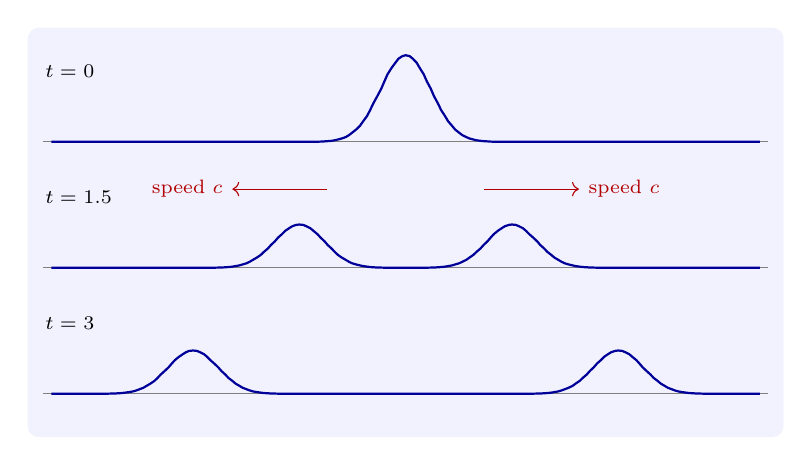
\begin{tikzpicture}[x=1cm,y=1cm]
\fill[blue!5,rounded corners=4pt] (-4.8,-3.75) rectangle (4.8,1.45);
\foreach \k/\t in {0/0, 1/1.5, 2/3} {
  \draw[black!50] (-4.6,-1.6*\k) -- (4.6,-1.6*\k);
  \node[font=\scriptsize,anchor=west] at (-4.7,-1.6*\k+0.9) {$t = \t$};
}
% t=0
\draw[blue!60!black,thick] (-4.50,0.000) -- (-4.46,0.000) -- (-4.41,0.000) -- (-4.37,0.000) -- (-4.32,0.000) -- (-4.28,0.000) -- (-4.23,0.000) -- (-4.19,0.000) -- (-4.14,0.000) -- (-4.09,0.000) -- (-4.05,0.000) -- (-4.00,0.000) -- (-3.96,0.000) -- (-3.91,0.000) -- (-3.87,0.000) -- (-3.83,0.000) -- (-3.78,0.000) -- (-3.74,0.000) -- (-3.69,0.000) -- (-3.65,0.000) -- (-3.60,0.000) -- (-3.56,0.000) -- (-3.51,0.000) -- (-3.46,0.000) -- (-3.42,0.000) -- (-3.38,0.000) -- (-3.33,0.000) -- (-3.29,0.000) -- (-3.24,0.000) -- (-3.19,0.000) -- (-3.15,0.000) -- (-3.11,0.000) -- (-3.06,0.000) -- (-3.01,0.000) -- (-2.97,0.000) -- (-2.93,0.000) -- (-2.88,0.000) -- (-2.83,0.000) -- (-2.79,0.000) -- (-2.75,0.000) -- (-2.70,0.000) -- (-2.65,0.000) -- (-2.61,0.000) -- (-2.56,0.000) -- (-2.52,0.000) -- (-2.48,0.000) -- (-2.43,0.000) -- (-2.38,0.000) -- (-2.34,0.000) -- (-2.29,0.000) -- (-2.25,0.000) -- (-2.20,0.000) -- (-2.16,0.000) -- (-2.11,0.000) -- (-2.07,0.000) -- (-2.02,0.000) -- (-1.98,0.000) -- (-1.94,0.000) -- (-1.89,0.000) -- (-1.84,0.000) -- (-1.80,0.000) -- (-1.75,0.000) -- (-1.71,0.000) -- (-1.66,0.000) -- (-1.62,0.000) -- (-1.57,0.000) -- (-1.53,0.000) -- (-1.48,0.000) -- (-1.44,0.000) -- (-1.39,0.000) -- (-1.35,0.000) -- (-1.30,0.000) -- (-1.26,0.000) -- (-1.21,0.001) -- (-1.17,0.001) -- (-1.12,0.002) -- (-1.08,0.003) -- (-1.03,0.006) -- (-0.99,0.009) -- (-0.94,0.013) -- (-0.90,0.020) -- (-0.86,0.030) -- (-0.81,0.043) -- (-0.76,0.061) -- (-0.72,0.085) -- (-0.68,0.116) -- (-0.63,0.155) -- (-0.58,0.203) -- (-0.54,0.261) -- (-0.49,0.328) -- (-0.45,0.405) -- (-0.41,0.489) -- (-0.36,0.580) -- (-0.31,0.674) -- (-0.27,0.767) -- (-0.23,0.857) -- (-0.18,0.937) -- (-0.13,1.005) -- (-0.09,1.057) -- (-0.04,1.089) -- (0.00,1.100) -- (0.05,1.089) -- (0.09,1.057) -- (0.14,1.005) -- (0.18,0.937) -- (0.23,0.857) -- (0.27,0.767) -- (0.32,0.674) -- (0.36,0.580) -- (0.41,0.489) -- (0.45,0.405) -- (0.50,0.328) -- (0.54,0.261) -- (0.59,0.203) -- (0.63,0.155) -- (0.68,0.116) -- (0.72,0.085) -- (0.77,0.061) -- (0.81,0.043) -- (0.86,0.030) -- (0.90,0.020) -- (0.95,0.013) -- (0.99,0.009) -- (1.04,0.006) -- (1.08,0.003) -- (1.12,0.002) -- (1.17,0.001) -- (1.22,0.001) -- (1.26,0.000) -- (1.31,0.000) -- (1.35,0.000) -- (1.40,0.000) -- (1.44,0.000) -- (1.49,0.000) -- (1.53,0.000) -- (1.57,0.000) -- (1.62,0.000) -- (1.67,0.000) -- (1.71,0.000) -- (1.76,0.000) -- (1.80,0.000) -- (1.85,0.000) -- (1.89,0.000) -- (1.94,0.000) -- (1.98,0.000) -- (2.02,0.000) -- (2.07,0.000) -- (2.12,0.000) -- (2.16,0.000) -- (2.21,0.000) -- (2.25,0.000) -- (2.30,0.000) -- (2.34,0.000) -- (2.39,0.000) -- (2.43,0.000) -- (2.48,0.000) -- (2.52,0.000) -- (2.57,0.000) -- (2.61,0.000) -- (2.66,0.000) -- (2.70,0.000) -- (2.75,0.000) -- (2.79,0.000) -- (2.84,0.000) -- (2.88,0.000) -- (2.93,0.000) -- (2.97,0.000) -- (3.01,0.000) -- (3.06,0.000) -- (3.11,0.000) -- (3.15,0.000) -- (3.20,0.000) -- (3.24,0.000) -- (3.29,0.000) -- (3.33,0.000) -- (3.38,0.000) -- (3.42,0.000) -- (3.46,0.000) -- (3.51,0.000) -- (3.56,0.000) -- (3.60,0.000) -- (3.65,0.000) -- (3.69,0.000) -- (3.74,0.000) -- (3.78,0.000) -- (3.83,0.000) -- (3.87,0.000) -- (3.91,0.000) -- (3.96,0.000) -- (4.01,0.000) -- (4.05,0.000) -- (4.10,0.000) -- (4.14,0.000) -- (4.19,0.000) -- (4.23,0.000) -- (4.28,0.000) -- (4.32,0.000) -- (4.37,0.000) -- (4.41,0.000) -- (4.46,0.000) -- (4.50,0.000);
% t=1.5
\draw[blue!60!black,thick] (-4.50,-1.600) -- (-4.46,-1.600) -- (-4.41,-1.600) -- (-4.37,-1.600) -- (-4.32,-1.600) -- (-4.28,-1.600) -- (-4.23,-1.600) -- (-4.19,-1.600) -- (-4.14,-1.600) -- (-4.09,-1.600) -- (-4.05,-1.600) -- (-4.00,-1.600) -- (-3.96,-1.600) -- (-3.91,-1.600) -- (-3.87,-1.600) -- (-3.83,-1.600) -- (-3.78,-1.600) -- (-3.74,-1.600) -- (-3.69,-1.600) -- (-3.65,-1.600) -- (-3.60,-1.600) -- (-3.56,-1.600) -- (-3.51,-1.600) -- (-3.46,-1.600) -- (-3.42,-1.600) -- (-3.38,-1.600) -- (-3.33,-1.600) -- (-3.29,-1.600) -- (-3.24,-1.600) -- (-3.19,-1.600) -- (-3.15,-1.600) -- (-3.11,-1.600) -- (-3.06,-1.600) -- (-3.01,-1.600) -- (-2.97,-1.600) -- (-2.93,-1.600) -- (-2.88,-1.600) -- (-2.83,-1.600) -- (-2.79,-1.600) -- (-2.75,-1.600) -- (-2.70,-1.600) -- (-2.65,-1.600) -- (-2.61,-1.600) -- (-2.56,-1.600) -- (-2.52,-1.599) -- (-2.48,-1.599) -- (-2.43,-1.598) -- (-2.38,-1.597) -- (-2.34,-1.596) -- (-2.29,-1.593) -- (-2.25,-1.590) -- (-2.20,-1.585) -- (-2.16,-1.578) -- (-2.11,-1.569) -- (-2.07,-1.557) -- (-2.02,-1.542) -- (-1.98,-1.523) -- (-1.94,-1.499) -- (-1.89,-1.470) -- (-1.84,-1.436) -- (-1.80,-1.398) -- (-1.75,-1.355) -- (-1.71,-1.310) -- (-1.66,-1.263) -- (-1.62,-1.216) -- (-1.57,-1.172) -- (-1.53,-1.131) -- (-1.48,-1.097) -- (-1.44,-1.072) -- (-1.39,-1.055) -- (-1.35,-1.050) -- (-1.30,-1.055) -- (-1.26,-1.072) -- (-1.21,-1.097) -- (-1.17,-1.131) -- (-1.12,-1.172) -- (-1.08,-1.216) -- (-1.03,-1.263) -- (-0.99,-1.310) -- (-0.94,-1.355) -- (-0.90,-1.398) -- (-0.86,-1.436) -- (-0.81,-1.470) -- (-0.76,-1.499) -- (-0.72,-1.523) -- (-0.68,-1.542) -- (-0.63,-1.557) -- (-0.58,-1.569) -- (-0.54,-1.578) -- (-0.49,-1.585) -- (-0.45,-1.590) -- (-0.41,-1.593) -- (-0.36,-1.596) -- (-0.31,-1.597) -- (-0.27,-1.598) -- (-0.23,-1.599) -- (-0.18,-1.599) -- (-0.13,-1.600) -- (-0.09,-1.600) -- (-0.04,-1.600) -- (0.00,-1.600) -- (0.05,-1.600) -- (0.09,-1.600) -- (0.14,-1.600) -- (0.18,-1.599) -- (0.23,-1.599) -- (0.27,-1.598) -- (0.32,-1.597) -- (0.36,-1.596) -- (0.41,-1.593) -- (0.45,-1.590) -- (0.50,-1.585) -- (0.54,-1.578) -- (0.59,-1.569) -- (0.63,-1.557) -- (0.68,-1.542) -- (0.72,-1.523) -- (0.77,-1.499) -- (0.81,-1.470) -- (0.86,-1.436) -- (0.90,-1.398) -- (0.95,-1.355) -- (0.99,-1.310) -- (1.04,-1.263) -- (1.08,-1.216) -- (1.12,-1.172) -- (1.17,-1.131) -- (1.22,-1.097) -- (1.26,-1.072) -- (1.31,-1.055) -- (1.35,-1.050) -- (1.40,-1.055) -- (1.44,-1.072) -- (1.49,-1.097) -- (1.53,-1.131) -- (1.57,-1.172) -- (1.62,-1.216) -- (1.67,-1.263) -- (1.71,-1.310) -- (1.76,-1.355) -- (1.80,-1.398) -- (1.85,-1.436) -- (1.89,-1.470) -- (1.94,-1.499) -- (1.98,-1.523) -- (2.02,-1.542) -- (2.07,-1.557) -- (2.12,-1.569) -- (2.16,-1.578) -- (2.21,-1.585) -- (2.25,-1.590) -- (2.30,-1.593) -- (2.34,-1.596) -- (2.39,-1.597) -- (2.43,-1.598) -- (2.48,-1.599) -- (2.52,-1.599) -- (2.57,-1.600) -- (2.61,-1.600) -- (2.66,-1.600) -- (2.70,-1.600) -- (2.75,-1.600) -- (2.79,-1.600) -- (2.84,-1.600) -- (2.88,-1.600) -- (2.93,-1.600) -- (2.97,-1.600) -- (3.01,-1.600) -- (3.06,-1.600) -- (3.11,-1.600) -- (3.15,-1.600) -- (3.20,-1.600) -- (3.24,-1.600) -- (3.29,-1.600) -- (3.33,-1.600) -- (3.38,-1.600) -- (3.42,-1.600) -- (3.46,-1.600) -- (3.51,-1.600) -- (3.56,-1.600) -- (3.60,-1.600) -- (3.65,-1.600) -- (3.69,-1.600) -- (3.74,-1.600) -- (3.78,-1.600) -- (3.83,-1.600) -- (3.87,-1.600) -- (3.91,-1.600) -- (3.96,-1.600) -- (4.01,-1.600) -- (4.05,-1.600) -- (4.10,-1.600) -- (4.14,-1.600) -- (4.19,-1.600) -- (4.23,-1.600) -- (4.28,-1.600) -- (4.32,-1.600) -- (4.37,-1.600) -- (4.41,-1.600) -- (4.46,-1.600) -- (4.50,-1.600);
% t=3.0
\draw[blue!60!black,thick] (-4.50,-3.200) -- (-4.46,-3.200) -- (-4.41,-3.200) -- (-4.37,-3.200) -- (-4.32,-3.200) -- (-4.28,-3.200) -- (-4.23,-3.200) -- (-4.19,-3.200) -- (-4.14,-3.200) -- (-4.09,-3.200) -- (-4.05,-3.200) -- (-4.00,-3.200) -- (-3.96,-3.200) -- (-3.91,-3.200) -- (-3.87,-3.199) -- (-3.83,-3.199) -- (-3.78,-3.198) -- (-3.74,-3.197) -- (-3.69,-3.196) -- (-3.65,-3.193) -- (-3.60,-3.190) -- (-3.56,-3.185) -- (-3.51,-3.178) -- (-3.46,-3.169) -- (-3.42,-3.157) -- (-3.38,-3.142) -- (-3.33,-3.123) -- (-3.29,-3.099) -- (-3.24,-3.070) -- (-3.19,-3.036) -- (-3.15,-2.998) -- (-3.11,-2.955) -- (-3.06,-2.910) -- (-3.01,-2.863) -- (-2.97,-2.816) -- (-2.93,-2.772) -- (-2.88,-2.731) -- (-2.83,-2.697) -- (-2.79,-2.672) -- (-2.75,-2.655) -- (-2.70,-2.650) -- (-2.65,-2.655) -- (-2.61,-2.672) -- (-2.56,-2.697) -- (-2.52,-2.731) -- (-2.48,-2.772) -- (-2.43,-2.816) -- (-2.38,-2.863) -- (-2.34,-2.910) -- (-2.29,-2.955) -- (-2.25,-2.998) -- (-2.20,-3.036) -- (-2.16,-3.070) -- (-2.11,-3.099) -- (-2.07,-3.123) -- (-2.02,-3.142) -- (-1.98,-3.157) -- (-1.94,-3.169) -- (-1.89,-3.178) -- (-1.84,-3.185) -- (-1.80,-3.190) -- (-1.75,-3.193) -- (-1.71,-3.196) -- (-1.66,-3.197) -- (-1.62,-3.198) -- (-1.57,-3.199) -- (-1.53,-3.199) -- (-1.48,-3.200) -- (-1.44,-3.200) -- (-1.39,-3.200) -- (-1.35,-3.200) -- (-1.30,-3.200) -- (-1.26,-3.200) -- (-1.21,-3.200) -- (-1.17,-3.200) -- (-1.12,-3.200) -- (-1.08,-3.200) -- (-1.03,-3.200) -- (-0.99,-3.200) -- (-0.94,-3.200) -- (-0.90,-3.200) -- (-0.86,-3.200) -- (-0.81,-3.200) -- (-0.76,-3.200) -- (-0.72,-3.200) -- (-0.68,-3.200) -- (-0.63,-3.200) -- (-0.58,-3.200) -- (-0.54,-3.200) -- (-0.49,-3.200) -- (-0.45,-3.200) -- (-0.41,-3.200) -- (-0.36,-3.200) -- (-0.31,-3.200) -- (-0.27,-3.200) -- (-0.23,-3.200) -- (-0.18,-3.200) -- (-0.13,-3.200) -- (-0.09,-3.200) -- (-0.04,-3.200) -- (0.00,-3.200) -- (0.05,-3.200) -- (0.09,-3.200) -- (0.14,-3.200) -- (0.18,-3.200) -- (0.23,-3.200) -- (0.27,-3.200) -- (0.32,-3.200) -- (0.36,-3.200) -- (0.41,-3.200) -- (0.45,-3.200) -- (0.50,-3.200) -- (0.54,-3.200) -- (0.59,-3.200) -- (0.63,-3.200) -- (0.68,-3.200) -- (0.72,-3.200) -- (0.77,-3.200) -- (0.81,-3.200) -- (0.86,-3.200) -- (0.90,-3.200) -- (0.95,-3.200) -- (0.99,-3.200) -- (1.04,-3.200) -- (1.08,-3.200) -- (1.12,-3.200) -- (1.17,-3.200) -- (1.22,-3.200) -- (1.26,-3.200) -- (1.31,-3.200) -- (1.35,-3.200) -- (1.40,-3.200) -- (1.44,-3.200) -- (1.49,-3.200) -- (1.53,-3.199) -- (1.57,-3.199) -- (1.62,-3.198) -- (1.67,-3.197) -- (1.71,-3.196) -- (1.76,-3.193) -- (1.80,-3.190) -- (1.85,-3.185) -- (1.89,-3.178) -- (1.94,-3.169) -- (1.98,-3.157) -- (2.02,-3.142) -- (2.07,-3.123) -- (2.12,-3.099) -- (2.16,-3.070) -- (2.21,-3.036) -- (2.25,-2.998) -- (2.30,-2.955) -- (2.34,-2.910) -- (2.39,-2.863) -- (2.43,-2.816) -- (2.48,-2.772) -- (2.52,-2.731) -- (2.57,-2.697) -- (2.61,-2.672) -- (2.66,-2.655) -- (2.70,-2.650) -- (2.75,-2.655) -- (2.79,-2.672) -- (2.84,-2.697) -- (2.88,-2.731) -- (2.93,-2.772) -- (2.97,-2.816) -- (3.01,-2.863) -- (3.06,-2.910) -- (3.11,-2.955) -- (3.15,-2.998) -- (3.20,-3.036) -- (3.24,-3.070) -- (3.29,-3.099) -- (3.33,-3.123) -- (3.38,-3.142) -- (3.42,-3.157) -- (3.46,-3.169) -- (3.51,-3.178) -- (3.56,-3.185) -- (3.60,-3.190) -- (3.65,-3.193) -- (3.69,-3.196) -- (3.74,-3.197) -- (3.78,-3.198) -- (3.83,-3.199) -- (3.87,-3.199) -- (3.91,-3.200) -- (3.96,-3.200) -- (4.01,-3.200) -- (4.05,-3.200) -- (4.10,-3.200) -- (4.14,-3.200) -- (4.19,-3.200) -- (4.23,-3.200) -- (4.28,-3.200) -- (4.32,-3.200) -- (4.37,-3.200) -- (4.41,-3.200) -- (4.46,-3.200) -- (4.50,-3.200);
\draw[->,red!70!black] (1.0,-0.6) -- (2.2,-0.6) node[right,font=\scriptsize] {speed $c$}; \draw[->,red!70!black] (-1.0,-0.6) -- (-2.2,-0.6) node[left,font=\scriptsize] {speed $c$};
\end{tikzpicture}
\caption{D'Alembert's solution with $f(x) = e^{-4x^2}$, $g = 0$ and $c = 1$, at three times. The initial pulse splits into two pulses of half the height, $\frac12f(x - t)$ and $\frac12f(x + t)$, travelling in opposite directions without change of shape.}
\label{fig:split}
\end{figure}

\subsection{Causality: domains of dependence and influence}
\label{ssec:causality}

Formula \eqref{eq:dalembert} shows that $u(x_0, t_0)$ depends only on the data in the interval $[x_0 - ct_0, x_0 + ct_0]$, the \textbf{domain of dependence} of the point, cut out by the two characteristics through it (Figure~\ref{fig:cones}). Conversely, data in an interval $[a, b]$ influence only the wedge
$a - ct \leq x \leq b + ct$, the \textbf{range of influence}. This is \textbf{finite speed of propagation}: a signal cannot travel faster than $c$.

There is a difference between the two kinds of data. Initial displacement $f$ affects only the edges of the range of influence: a pulse in $f$ passes a point and is gone. Initial velocity $g$ enters through an integral, so its effect fills the whole wedge: a string struck by a hammer
is left permanently displaced behind the waves (Problem~\ref{prob:hammer}). In one dimension, the sharp form of Huygens' principle fails; whether it holds depends on the dimension, as the next section shows.

\begin{figure}[H]
\centering
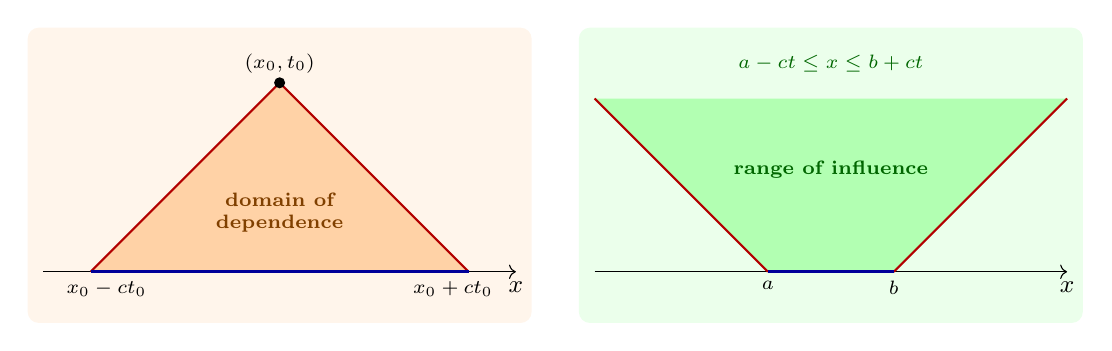
\begin{tikzpicture}[x=1cm,y=1cm]
\begin{scope}
\fill[orange!8,rounded corners=4pt] (-3.2,-0.65) rectangle (3.2,3.1);
\draw[->] (-3,0) -- (3,0) node[below,font=\small] {$x$};
\fill[orange!35] (0,2.4) -- (-2.4,0) -- (2.4,0) -- cycle;
\draw[red!70!black,thick] (-2.4,0) -- (0,2.4) -- (2.4,0);
\fill (0,2.4) circle (2pt) node[above,font=\scriptsize] {$(x_0, t_0)$};
\draw[very thick,blue!60!black] (-2.4,0) -- (2.4,0);
\node[font=\scriptsize,below] at (-2.2,0) {$x_0 - ct_0$}; \node[font=\scriptsize,below] at (2.2,0) {$x_0 + ct_0$};
\node[font=\scriptsize\bfseries,orange!50!black,align=center] at (0,0.75) {domain of\\dependence};
\end{scope}
\begin{scope}[shift={(7,0)}]
\fill[green!8,rounded corners=4pt] (-3.2,-0.65) rectangle (3.2,3.1);
\draw[->] (-3,0) -- (3,0) node[below,font=\small] {$x$};
\fill[green!30] (-0.8,0) -- (-3,2.2) -- (3,2.2) -- (0.8,0) -- cycle;
\draw[red!70!black,thick] (-0.8,0) -- (-3,2.2); \draw[red!70!black,thick] (0.8,0) -- (3,2.2);
\draw[very thick,blue!60!black] (-0.8,0) -- (0.8,0);
\node[font=\scriptsize,below] at (-0.8,0) {$a$}; \node[font=\scriptsize,below] at (0.8,0) {$b$};
\node[font=\scriptsize\bfseries,green!40!black] at (0,1.3) {range of influence};
\node[font=\scriptsize,green!40!black] at (0,2.65) {$a - ct \leq x \leq b + ct$};
\end{scope}
\end{tikzpicture}
\caption{Causality for the wave equation. Left: the value at $(x_0, t_0)$ depends only on the data between the two characteristics $x \pm ct = x_0 \pm ct_0$ through the point. Right: data on $[a, b]$ affect only the region between the outgoing characteristics; outside it, the solution
does not know they exist.}
\label{fig:cones}
\end{figure}

\subsection{Energy}
\label{ssec:energy1d}

\begin{thm}[Conservation of energy]
\label{thm:energy1d}
Let $u$ be a $C^2$ solution of \eqref{eq:wave1d} for which $u_t$ and $u_x$ vanish for large $|x|$. Then the energy
\[
E(t) = \frac12\int_{-\infty}^\infty\bigl(u_t^2 + c^2u_x^2\bigr)\,dx
\]
is constant. More generally, for any $a < b$ the energy in the shrinking interval $[a + ct, b - ct]$ is non-increasing for $0 \leq t \leq (b - a)/2c$.
\end{thm}

\begin{proof}
Let $e = \frac12(u_t^2 + c^2u_x^2)$. Then $e_t = u_tu_{tt} + c^2u_xu_{xt} = c^2(u_tu_{xx} + u_xu_{xt}) = c^2(u_tu_x)_x$, so $dE/dt = c^2[u_tu_x]_{-\infty}^\infty = 0$. For the shrinking interval, by Leibniz's rule,
\[
\frac{d}{dt}\int_{a + ct}^{b - ct}e\,dx = c^2\bigl[u_tu_x\bigr]_{a + ct}^{b - ct} - c\,e(b - ct) - c\,e(a + ct) ,
\]
and $|c^2u_tu_x| \leq c\cdot\frac12(u_t^2 + c^2u_x^2) = c\,e$, so each endpoint contributes at most $0$.
\end{proof}

The second statement gives uniqueness and finite speed of propagation without any formula. If two solutions agree initially on $[a, b]$, their difference has zero energy there at $t = 0$, hence zero energy on the shrinking interval, hence $u_t = u_x = 0$ and the difference vanishes in the
triangle: this is the domain of dependence again. The argument works for variable coefficients and in any dimension, where no d'Alembert formula exists, and it is the model for the energy methods of a later section.

\subsection{Sources: Duhamel's principle}
\label{ssec:duhamel1d}

\begin{thm}
\label{thm:duhamel1d}
If $F$ is $C^1$, the solution of $u_{tt} = c^2u_{xx} + F(x, t)$ with $u(x, 0) = u_t(x, 0) = 0$ is
\[
u(x, t) = \frac1{2c}\int_0^t\!\!\int_{x - c(t - s)}^{x + c(t - s)}F(y, s)\,dy\,ds ,
\]
the integral of $F$ over the characteristic triangle below $(x, t)$, divided by $2c$.
\end{thm}

\begin{proof}
For each $s$, let $v(\cdot, \cdot; s)$ solve the homogeneous equation for $t > s$ with $v = 0$ and $v_t = F(\cdot, s)$ at $t = s$; by d'Alembert, $v(x, t; s) = \frac1{2c}\int_{x - c(t - s)}^{x + c(t - s)}F(y, s)\,dy$. Put $u = \int_0^tv(x, t; s)\,ds$. Then $u_t = v(x, t; t) + \int_0^tv_t\,ds = \int_0^tv_t\,ds$, since $v(x, s; s) = 0$, and
\[
u_{tt} = v_t(x, t; t) + \int_0^tv_{tt}\,ds = F(x, t) + c^2\int_0^tv_{xx}\,ds = F + c^2u_{xx} .
\]
The initial conditions hold since both integrals vanish at $t = 0$.
\end{proof}

The idea, Duhamel's principle, is that a source acting over time is a succession of impulses, each of which sets off a solution of the homogeneous problem, as for the transport equation in Section~\ref{sec:characteristics}. With non-zero data, add the d'Alembert solution.

\subsection{Boundaries and reflection}
\label{ssec:reflection}

On the half-line $x > 0$ with a fixed end, $u(0, t) = 0$, extend $f$ and $g$ to odd functions on $\mathbb R$. The d'Alembert solution of the extended problem is odd in $x$, so it vanishes at $x = 0$, and by uniqueness it is the solution. For $x \geq ct$ the extension plays no part, and for $0 \leq x < ct$,
\[
u(x, t) = \frac12\bigl(f(x + ct) - f(ct - x)\bigr) + \frac1{2c}\int_{ct - x}^{x + ct}g(y)\,dy .
\]
A wave arriving at a fixed end is reflected upside down. For a free end, $u_x(0, t) = 0$, the even extension gives a reflection the right way up. On a finite string $0 \leq x \leq L$ with both ends fixed, the odd $2L$-periodic extension of the data gives the solution, which is therefore periodic in time with period
$2L/c$: the fundamental frequency of the string is $c/2L = \sqrt{T/\rho}/2L$, Mersenne's law. The decomposition into the overtones $\sin(k\pi x/L)$, of frequencies $kc/2L$, is the subject of the section on Fourier series.

\subsection{The wave equation in software}
\label{ssec:software4}

\begin{software}[D'Alembert and Duhamel]
\label{sw:dalembert}
A symbolic check of \eqref{eq:dalembert} for arbitrary $f$ and $g$, and the Duhamel integral of Theorem~\ref{thm:duhamel1d} for the source $F = xt$:
{\small\begin{verbatim}
>>> import sympy as sp
>>> x, t, s, y, c = sp.symbols('x t s y c', positive=True)
>>> f, g = sp.Function('f'), sp.Function('g')
>>> u = ((f(x + c*t) + f(x - c*t)) / 2
...      + sp.Integral(g(y), (y, x - c*t, x + c*t)) / (2*c))
>>> sp.simplify(u.diff(t, 2) - c**2 * u.diff(x, 2))          # d'Alembert
0
>>> u.subs(t, 0).doit(), sp.simplify(u.diff(t).subs(t, 0).doit())
(f(x), g(x))
>>> F = lambda y, s: y * s                 # forcing in u_tt = c^2 u_xx + F
>>> inner = sp.integrate(F(y, s), (y, x - c*(t - s), x + c*(t - s)))
>>> w = sp.integrate(inner, (s, 0, t)) / (2*c)   # Duhamel: over the triangle
>>> sp.factor(w), sp.simplify(w.diff(t, 2) - c**2 * w.diff(x, 2))
(t**3*x/6, t*x)
\end{verbatim}}
\textbf{Reading the output.} D'Alembert's formula satisfies the equation identically and takes the right initial values. The Duhamel integral over the triangle gives $u = xt^3/6$, and $u_{tt} - c^2u_{xx} = xt$ returns the source.

\textbf{MATLAB/Octave:} with the Symbolic Math Toolbox, \texttt{int(int(y*s, y, x-c*(t-s), x+c*(t-s)), s, 0, t)/(2*c)}.
\end{software}

\begin{software}[Energy of a plucked string]
\label{sw:pluck}
A string of length $1$, with $c = 1$ and fixed ends, plucked at $x = 0.3$ to a height of $0.01$ and released, is solved by the leapfrog scheme $u_j^{n+1} = 2u_j^n - u_j^{n-1} + r^2(u_{j+1}^n - 2u_j^n + u_{j-1}^n)$ with $r = c\,\Delta t/\Delta x = \frac12$. The energy is computed in the form that the scheme
conserves exactly, $\frac12\sum\bigl((u_j^{n+1} - u_j^n)/\Delta t\bigr)^2\Delta x + \frac12\sum(u_{j+1}^{n+1} - u_j^{n+1})(u_{j+1}^n - u_j^n)/\Delta x$:
{\small\begin{verbatim}
>>> import numpy as np
>>> def leapfrog(u0, r, steps, ends='fixed'):   # u_tt = u_xx, r = c dt / dx
...     uo = u0.copy(); un = u0.copy()
...     un[1:-1] += 0.5 * r**2 * (u0[2:] - 2*u0[1:-1] + u0[:-2])
...     for _ in range(steps - 1):
...         nxt = np.empty_like(un)
...         nxt[1:-1] = (2*un[1:-1] - uo[1:-1]
...                      + r**2 * (un[2:] - 2*un[1:-1] + un[:-2]))
...         nxt[0] = 0 if ends == 'fixed' else nxt[1]      # u = 0 or u_x = 0
...         nxt[-1] = 0
...         uo, un = un, nxt
...     return uo, un
...
>>> x = np.linspace(0, 1, 401); dx = x[1]                  # string, L = c = 1
>>> u0 = 0.01 * np.where(x < 0.3, x / 0.3, (1 - x) / 0.7)  # plucked at 0.3
>>> 0.5 * np.sum(np.diff(u0)**2) / dx      # energy = (1/2) int u_x^2 at rest
0.00023809523809523812
>>> for steps in (400, 800, 1600):         # t = 0.5, 1, 2 with r = 1/2
...     uo, un = leapfrog(u0, 0.5, steps); dt = 0.5 * dx
...     E = 0.5 * np.sum(((un - uo) / dt)**2) * dx \
...         + 0.5 * np.sum(np.diff(un) * np.diff(uo)) / dx
...     print(steps * dt, f"{E:.6e}", round(float(np.abs(un - u0).max()), 6))
...
0.5 2.379181e-04 0.011906
1.0 2.379181e-04 0.014325
2.0 2.379181e-04 0.000128
\end{verbatim}}
\textbf{Reading the output.} The exact energy is $\frac12\int f'^2 = \frac12(0.01)^2(\frac1{0.3} + \frac1{0.7}) = 2.381 \times 10^{-4}$. The computed energy, $2.379181 \times 10^{-4}$, is the same to all seven digits at $t = 0.5$, $1$ and $2$; it differs from the exact value by $0.07\%$, an error made by the
starting step. The last column is the largest distance from the initial shape: large at $t = 0.5$ and $t = 1$, and $1.3 \times 10^{-4}$, about $1\%$ of the amplitude, at $t = 2 = 2L/c$, when the string has returned to where it started.

\textbf{MATLAB/Octave:} the same loop with \texttt{u(2:end-1)} indexing.
\end{software}

\begin{software}[Reflection at fixed and free ends]
\label{sw:reflect}
A pulse $e^{-50(x - 2)^2}$, released from rest on the half-line, with a fixed end ($u = 0$) and with a free end ($u_x = 0$) at $x = 0$; the solution at $t = 3$:
{\small\begin{verbatim}
>>> x = np.linspace(0, 6, 1201); dx = x[1]  # half-line, cut at 6
>>> pulse = lambda z: np.exp(-50 * (z - 2)**2)  # starts at rest at 2
>>> for ends in ('fixed', 'free'):
...     _, u = leapfrog(pulse(x), 0.5, 1200, ends)  # t = 1200 dx / 2 = 3
...     print(ends, np.round(np.interp([0.5, 1.0, 1.5, 5.0], x, u), 4))
...
fixed [-0.  -0.5 -0.   0.5]
free [0.     0.4995 0.     0.5   ]
\end{verbatim}}
\textbf{Reading the output.} The pulse splits into two halves of height $\frac12$. The right-moving half is at $x = 2 + 3 = 5$. The left-moving half reached the end at $t = 2$ and has come back to $x = 1$, upside down ($-0.5$) at the fixed end and the right way up ($0.4995$) at the free end, as the odd and even
extensions predict.

\textbf{MATLAB/Octave:} the same scheme, with \texttt{u(1) = u(2)} for the free end.
\end{software}

\subsection{Practice Problems}

\begin{problem}
Solve $u_{tt} = 4u_{xx}$ with $u(x, 0) = \sin x$ and $u_t(x, 0) = \cos x$.
\end{problem}

\begin{solution}
With $c = 2$,
\[
u = \tfrac12\bigl(\sin(x + 2t) + \sin(x - 2t)\bigr) + \tfrac14\bigl(\sin(x + 2t) - \sin(x - 2t)\bigr) = \sin x\cos 2t + \tfrac12\cos x\sin 2t .
\]
Check: $u_t(x, 0) = \cos x\cos 0 = \cos x$.
\end{solution}

\begin{problem}
\label{prob:hammer}
A string with $c = 1$, at rest and undisplaced, is struck so that $u_t(x, 0) = 1$ for $|x| < 1$ and $0$ otherwise. Find $u(0, t)$ for all $t > 0$, and $u(x, t)$ for large $t$.
\end{problem}

\begin{solution}
$u(0, t) = \frac12\int_{-t}^tg = \frac12\cdot 2\min(t, 1) = \min(t, 1)$: the centre rises steadily until $t = 1$ and then stays at height $1$. In general $u(x, t) = \frac12\,\bigl|[x - t, x + t] \cap [-1, 1]\bigr|$, which for $t > 1 + |x|$ is $1$: the string is left permanently displaced by $1$ over an
expanding interval $|x| < t - 1$, with ramps at its edges. The disturbance does not pass.
\end{solution}

\begin{problem}
Use the energy to prove that the problem $u_{tt} = c^2u_{xx}$ on $0 < x < L$, $u(0, t) = u(L, t) = 0$, with given $u(x, 0)$ and $u_t(x, 0)$, has at most one $C^2$ solution.
\end{problem}

\begin{solution}
The difference $w$ of two solutions has zero data. Its energy $E(t) = \frac12\int_0^L(w_t^2 + c^2w_x^2)\,dx$ has $E'(t) = c^2[w_tw_x]_0^L = 0$, since $w = 0$ at the ends for all $t$ implies $w_t = 0$ there. So $E(t) = E(0) = 0$, hence $w_t = w_x = 0$, $w$ is constant, and $w = 0$ since it vanishes at $x = 0$.
\end{solution}

\begin{problem}
Solve $u_{tt} = u_{xx} + \sin x$ with $u(x, 0) = u_t(x, 0) = 0$.
\end{problem}

\begin{solution}
By Duhamel,
\[
u = \frac12\int_0^t\bigl(\cos(x - (t - s)) - \cos(x + (t - s))\bigr)ds = \int_0^t\sin x\sin(t - s)\,ds = \sin x\,(1 - \cos t) .
\]
Check: $u_{tt} = \sin x\cos t$ and $u_{xx} + \sin x = -\sin x(1 - \cos t) + \sin x = \sin x\cos t$.
\end{solution}

\begin{problem}
A guitar string $0.65$\,m long has fundamental frequency $196$\,Hz. Find the wave speed $c$, and the tension if the linear density is $3.1 \times 10^{-3}$\,kg/m.
\end{problem}

\begin{solution}
From $c/2L = 196$, $c = 2 \times 0.65 \times 196 = 254.8$\,m/s, and $T = \rho c^2 = 3.1 \times 10^{-3} \times 254.8^2 = 201$\,N.
\end{solution}

\begin{problem}
For the half-line problem with a fixed end, $f = 0$ and $g(x) = 1$ for $1 < x < 2$, $0$ otherwise, $c = 1$, find $u(\frac12, t)$ for $t > 0$.
\end{problem}

\begin{solution}
For $t \leq \frac12$, $u = \frac12\int_{1/2 - t}^{1/2 + t}g = 0$, since the interval lies below $1$. For $t > \frac12$, $u = \frac12\int_{t - 1/2}^{t + 1/2}g$, the half-length of $[t - \frac12, t + \frac12] \cap [1, 2]$: it is $\frac12(t - \frac12)$ for $\frac12 \leq t \leq \frac32$, $\frac12(\frac52 - t)$ for $\frac32 \leq t \leq \frac52$, and $0$ after. The point is
first reached by the left-moving disturbance at $t = \frac12$, and once the wave reflected from the fixed end has passed, it returns to rest: the reflected wave, from the odd extension, cancels the permanent displacement of Problem~\ref{prob:hammer}.
\end{solution}

%======================================================================
\section{Waves in Higher Dimensions}
\label{sec:waveshigher}

In two and three dimensions the wave equation
\[
u_{tt} = c^2\Delta u
\]
still propagates disturbances at speed $c$ and conserves energy, but a new phenomenon appears: the dimension decides whether a signal passes cleanly. In three dimensions a flash of light or a clap is seen or heard for exactly as long as it lasted, and then there is silence; in two
dimensions a disturbance leaves a wake that dies away only slowly, as the ripples on a pond show. This is \textbf{Huygens' principle} in its sharp form. It follows from the explicit solution formulas of Kirchhoff and Poisson, which this section derives.

\subsection{Spherical means and Kirchhoff's formula}
\label{ssec:sphericalmeans}

For a continuous function $h$ on $\mathbb R^n$, the \textbf{spherical mean} of $h$ over the sphere of radius $r$ about $x$ is
\[
M_h(x, r) = \frac{1}{\omega_n}\int_{|\omega| = 1}h(x + r\omega)\,dS(\omega) ,
\]
where $\omega_n$ is the area of the unit sphere ($4\pi$ in $\mathbb R^3$). As $r \to 0$, $M_h(x, r) \to h(x)$.

\begin{lem}[Darboux]
\label{lem:darboux}
If $h$ is $C^2$, then $\partial_r^2M_h + \frac{n - 1}{r}\partial_rM_h = \Delta_xM_h$.
\end{lem}

\begin{proof}
Differentiating under the integral and applying the divergence theorem on the ball $B_r(x)$,
\[
\partial_rM_h = \frac1{\omega_n}\int_{|\omega| = 1}\nabla h(x + r\omega)\cdot\omega\,dS = \frac{1}{\omega_nr^{n - 1}}\int_{B_r(x)}\Delta h\,dy .
\]
So $r^{n - 1}\partial_rM_h = \frac1{\omega_n}\int_{B_r(x)}\Delta h$, and differentiating in $r$ gives $\partial_r(r^{n - 1}\partial_rM_h) = \frac1{\omega_n}\int_{\partial B_r(x)}\Delta h\,dS = r^{n - 1}M_{\Delta h}(x, r) = r^{n - 1}\Delta_xM_h$, which is the identity.
\end{proof}

If $u$ solves the wave equation, apply the lemma to $h = u(\cdot, t)$: the mean $U(x; r, t) = M_{u(\cdot, t)}(x, r)$ satisfies the \textbf{Euler--Poisson--Darboux equation}
\[
U_{tt} = c^2\Bigl(U_{rr} + \frac{n - 1}{r}U_r\Bigr) .
\]
In three dimensions the substitution $V = rU$ turns this into $V_{tt} = c^2V_{rr}$, the one-dimensional wave equation, on the half-line $r > 0$ with $V(x; 0, t) = 0$. The same calculation shows that the radial solutions in $\mathbb R^3$ are the \textbf{spherical waves}
\[
u = \frac{F(r - ct) + G(r + ct)}{r} ,
\]
outgoing and incoming, whose amplitude decays like $1/r$ so that the energy crossing each sphere, proportional to $r^2\cdot r^{-2}$, is the same.

\begin{thm}[Kirchhoff]
\label{thm:kirchhoff}
Let $f \in C^3(\mathbb R^3)$ and $g \in C^2(\mathbb R^3)$. The solution of $u_{tt} = c^2\Delta u$ in $\mathbb R^3$ with $u(x, 0) = f$, $u_t(x, 0) = g$ is
\[
u(x, t) = \frac{\partial}{\partial t}\bigl(tM_f(x, ct)\bigr) + tM_g(x, ct) ,
\]
that is,
\[
u(x, t) = \frac{\partial}{\partial t}\biggl(\frac{1}{4\pi c^2t}\int_{|y - x| = ct}f\,dS\biggr) + \frac{1}{4\pi c^2t}\int_{|y - x| = ct}g\,dS .
\]
\end{thm}

\begin{proof}
With $V = rU$ as above, $V(x; r, 0) = rM_f(x, r) =: \Phi(r)$ and $V_t(x; r, 0) = rM_g(x, r) =: \Psi(r)$, both odd in $r$ when extended to $r < 0$. By the reflection formula of Section~\ref{sec:wave1d}, for $0 < r < ct$,
\[
V(x; r, t) = \frac12\bigl(\Phi(ct + r) - \Phi(ct - r)\bigr) + \frac1{2c}\int_{ct - r}^{ct + r}\Psi(s)\,ds .
\]
Since $u(x, t) = \lim_{r \to 0}U = \lim_{r \to 0}V/r$, dividing by $r$ and letting $r \to 0$ gives $u = \Phi'(ct) + \frac1c\Psi(ct)$. Now $\Phi'(ct) = \frac{d}{d\rho}\bigl(\rho M_f(x, \rho)\bigr)\big|_{\rho = ct} = \frac{\partial}{\partial t}\bigl(tM_f(x, ct)\bigr)$ and $\frac1c\Psi(ct) = tM_g(x, ct)$. The
hypotheses make $u$ a $C^2$ solution; the loss of one derivative from $f$ to $u$ is a feature of waves in three dimensions, where focusing can amplify singularities.
\end{proof}

\subsection{Poisson's formula by descent}
\label{ssec:descent}

A solution in two dimensions is a solution in three that does not depend on $x_3$. Hadamard's \textbf{method of descent} applies Kirchhoff's formula to such data. The sphere $|y - x| = ct$ in $\mathbb R^3$, with $x$ in the plane $x_3 = 0$, projects twice onto the disc $|y - x| < ct$ in the plane, with area element
$dS = ct\,dy/\sqrt{c^2t^2 - |y - x|^2}$, so $\frac1{4\pi c^2t}\int_{\text{sphere}}g\,dS = \frac{1}{2\pi c}\int_{\text{disc}}g(y)/\sqrt{c^2t^2 - |y - x|^2}\,dy$.

\begin{thm}[Poisson]
\label{thm:poisson2d}
In $\mathbb R^2$ the solution of $u_{tt} = c^2\Delta u$, $u(x, 0) = f$, $u_t(x, 0) = g$, is
\[
u(x, t) = \frac{\partial}{\partial t}\biggl(\frac{1}{2\pi c}\int_{|y - x| < ct}\frac{f(y)\,dy}{\sqrt{c^2t^2 - |y - x|^2}}\biggr) + \frac{1}{2\pi c}\int_{|y - x| < ct}\frac{g(y)\,dy}{\sqrt{c^2t^2 - |y - x|^2}} .
\]
\end{thm}

Descending once more, to data depending on $x_1$ only, and using $\int_{-h}^h dy_2/\sqrt{h^2 - y_2^2} = \pi$, recovers d'Alembert's term $\frac1{2c}\int_{x - ct}^{x + ct}g$ (Problem~\ref{prob:descent}).

\subsection{Huygens' principle}
\label{ssec:huygens}

Compare the two formulas. In three dimensions $u(x, t)$ depends only on the data on the \emph{sphere} $|y - x| = ct$; in two dimensions it depends on the data in the whole \emph{disc} $|y - x| \leq ct$. So if the data vanish outside a ball of radius $a$, then in three dimensions $u(x, t) = 0$ except when
$|x| - a \leq ct \leq |x| + a$: the signal arrives, lasts for time $2a/c$, and is gone. This is the \textbf{sharp Huygens principle}. In two dimensions, once the signal has arrived, every later disc contains the support of the data and $u$ is never again identically zero there: the disturbance leaves a wake.

\begin{exa}
\label{ex:huygens}
Take $f = 0$ and $g = 1$ in the ball $|y| < a$ (a sudden blow to a small region), and $c = 1$. In three dimensions, at a point with $|x| = R > a$, the fraction of the sphere of radius $t$ about $x$ inside the ball is $\bigl(a^2 - (R - t)^2\bigr)/4Rt$ for $|R - t| < a$, so
\[
u(x, t) = \frac{a^2 - (R - t)^2}{4R} \quad (|R - t| < a), \qquad u = 0 \text{ otherwise}:
\]
a single pulse of height $a^2/4R$. In two dimensions, at the centre, Poisson's formula gives $u = t$ for $t \leq a$ and $u = t - \sqrt{t^2 - a^2}$ for $t > a$, which decays only like $a^2/2t$ (Figure~\ref{fig:huygens}).
\end{exa}

\begin{figure}[H]
\centering
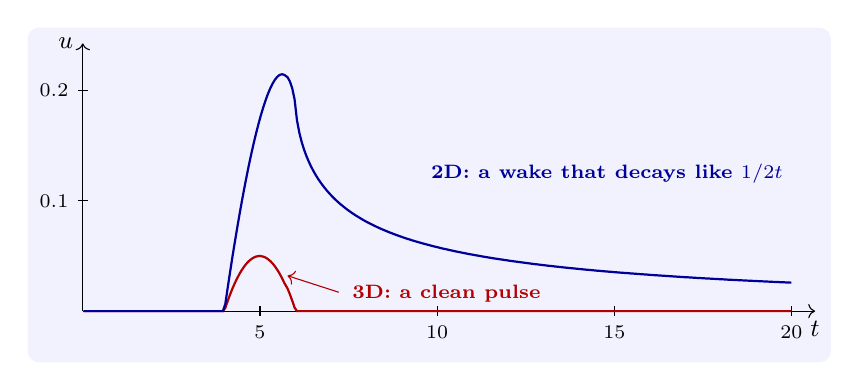
\begin{tikzpicture}[x=1cm,y=1cm]
\fill[blue!5,rounded corners=4pt] (-0.7,-0.65) rectangle (9.5,3.6);
\draw[->] (0,0) -- (9.3,0) node[below,font=\small] {$t$};
\draw[->] (0,0) -- (0,3.4) node[left,font=\small] {$u$};
\foreach \t in {5,10,15,20} \draw ({0.45*\t},0.06) -- ({0.45*\t},-0.06) node[below,font=\scriptsize] {$\t$};
\foreach \u in {0.1,0.2} \draw (0.06,{14*\u}) -- (-0.06,{14*\u}) node[left,font=\scriptsize] {$\u$};
\draw[red!70!black,thick] (0.01,0.000) -- (0.04,0.000) -- (0.07,0.000) -- (0.10,0.000) -- (0.13,0.000) -- (0.16,0.000) -- (0.19,0.000) -- (0.22,0.000) -- (0.25,0.000) -- (0.28,0.000) -- (0.31,0.000) -- (0.34,0.000) -- (0.37,0.000) -- (0.40,0.000) -- (0.43,0.000) -- (0.46,0.000) -- (0.49,0.000) -- (0.52,0.000) -- (0.55,0.000) -- (0.58,0.000) -- (0.61,0.000) -- (0.64,0.000) -- (0.67,0.000) -- (0.70,0.000) -- (0.73,0.000) -- (0.76,0.000) -- (0.79,0.000) -- (0.82,0.000) -- (0.85,0.000) -- (0.88,0.000) -- (0.91,0.000) -- (0.94,0.000) -- (0.97,0.000) -- (1.00,0.000) -- (1.03,0.000) -- (1.06,0.000) -- (1.09,0.000) -- (1.12,0.000) -- (1.15,0.000) -- (1.18,0.000) -- (1.21,0.000) -- (1.24,0.000) -- (1.27,0.000) -- (1.30,0.000) -- (1.33,0.000) -- (1.36,0.000) -- (1.39,0.000) -- (1.42,0.000) -- (1.45,0.000) -- (1.48,0.000) -- (1.51,0.000) -- (1.54,0.000) -- (1.57,0.000) -- (1.60,0.000) -- (1.63,0.000) -- (1.66,0.000) -- (1.69,0.000) -- (1.72,0.000) -- (1.75,0.000) -- (1.78,0.000) -- (1.81,0.041) -- (1.84,0.128) -- (1.87,0.210) -- (1.90,0.285) -- (1.93,0.354) -- (1.96,0.416) -- (1.99,0.473) -- (2.02,0.523) -- (2.05,0.567) -- (2.08,0.605) -- (2.11,0.636) -- (2.14,0.661) -- (2.17,0.680) -- (2.20,0.693) -- (2.23,0.699) -- (2.26,0.699) -- (2.29,0.693) -- (2.32,0.681) -- (2.35,0.662) -- (2.38,0.637) -- (2.41,0.606) -- (2.44,0.569) -- (2.47,0.525) -- (2.50,0.476) -- (2.53,0.419) -- (2.56,0.357) -- (2.60,0.288) -- (2.63,0.214) -- (2.66,0.132) -- (2.69,0.045) -- (2.72,0.000) -- (2.75,0.000) -- (2.78,0.000) -- (2.81,0.000) -- (2.84,0.000) -- (2.87,0.000) -- (2.90,0.000) -- (2.93,0.000) -- (2.96,0.000) -- (2.99,0.000) -- (3.02,0.000) -- (3.05,0.000) -- (3.08,0.000) -- (3.11,0.000) -- (3.14,0.000) -- (3.17,0.000) -- (3.20,0.000) -- (3.23,0.000) -- (3.26,0.000) -- (3.29,0.000) -- (3.32,0.000) -- (3.35,0.000) -- (3.38,0.000) -- (3.41,0.000) -- (3.44,0.000) -- (3.47,0.000) -- (3.50,0.000) -- (3.53,0.000) -- (3.56,0.000) -- (3.59,0.000) -- (3.62,0.000) -- (3.65,0.000) -- (3.68,0.000) -- (3.71,0.000) -- (3.74,0.000) -- (3.77,0.000) -- (3.80,0.000) -- (3.83,0.000) -- (3.86,0.000) -- (3.89,0.000) -- (3.92,0.000) -- (3.95,0.000) -- (3.98,0.000) -- (4.01,0.000) -- (4.04,0.000) -- (4.07,0.000) -- (4.10,0.000) -- (4.13,0.000) -- (4.16,0.000) -- (4.19,0.000) -- (4.22,0.000) -- (4.25,0.000) -- (4.28,0.000) -- (4.31,0.000) -- (4.34,0.000) -- (4.37,0.000) -- (4.40,0.000) -- (4.43,0.000) -- (4.46,0.000) -- (4.49,0.000) -- (4.52,0.000) -- (4.55,0.000) -- (4.58,0.000) -- (4.61,0.000) -- (4.64,0.000) -- (4.67,0.000) -- (4.70,0.000) -- (4.73,0.000) -- (4.76,0.000) -- (4.79,0.000) -- (4.82,0.000) -- (4.85,0.000) -- (4.88,0.000) -- (4.91,0.000) -- (4.94,0.000) -- (4.97,0.000) -- (5.00,0.000) -- (5.03,0.000) -- (5.06,0.000) -- (5.09,0.000) -- (5.12,0.000) -- (5.15,0.000) -- (5.18,0.000) -- (5.21,0.000) -- (5.24,0.000) -- (5.27,0.000) -- (5.30,0.000) -- (5.33,0.000) -- (5.36,0.000) -- (5.39,0.000) -- (5.42,0.000) -- (5.45,0.000) -- (5.48,0.000) -- (5.51,0.000) -- (5.54,0.000) -- (5.57,0.000) -- (5.60,0.000) -- (5.63,0.000) -- (5.66,0.000) -- (5.69,0.000) -- (5.72,0.000) -- (5.75,0.000) -- (5.78,0.000) -- (5.81,0.000) -- (5.84,0.000) -- (5.87,0.000) -- (5.90,0.000) -- (5.93,0.000) -- (5.96,0.000) -- (5.99,0.000) -- (6.02,0.000) -- (6.05,0.000) -- (6.08,0.000) -- (6.11,0.000) -- (6.14,0.000) -- (6.17,0.000) -- (6.20,0.000) -- (6.23,0.000) -- (6.26,0.000) -- (6.29,0.000) -- (6.32,0.000) -- (6.35,0.000) -- (6.38,0.000) -- (6.41,0.000) -- (6.44,0.000) -- (6.47,0.000) -- (6.50,0.000) -- (6.53,0.000) -- (6.56,0.000) -- (6.59,0.000) -- (6.62,0.000) -- (6.65,0.000) -- (6.68,0.000) -- (6.71,0.000) -- (6.74,0.000) -- (6.77,0.000) -- (6.80,0.000) -- (6.83,0.000) -- (6.87,0.000) -- (6.90,0.000) -- (6.93,0.000) -- (6.96,0.000) -- (6.99,0.000) -- (7.02,0.000) -- (7.05,0.000) -- (7.08,0.000) -- (7.11,0.000) -- (7.14,0.000) -- (7.17,0.000) -- (7.20,0.000) -- (7.23,0.000) -- (7.26,0.000) -- (7.29,0.000) -- (7.32,0.000) -- (7.35,0.000) -- (7.38,0.000) -- (7.41,0.000) -- (7.44,0.000) -- (7.47,0.000) -- (7.50,0.000) -- (7.53,0.000) -- (7.56,0.000) -- (7.59,0.000) -- (7.62,0.000) -- (7.65,0.000) -- (7.68,0.000) -- (7.71,0.000) -- (7.74,0.000) -- (7.77,0.000) -- (7.80,0.000) -- (7.83,0.000) -- (7.86,0.000) -- (7.89,0.000) -- (7.92,0.000) -- (7.95,0.000) -- (7.98,0.000) -- (8.01,0.000) -- (8.04,0.000) -- (8.07,0.000) -- (8.10,0.000) -- (8.13,0.000) -- (8.16,0.000) -- (8.19,0.000) -- (8.22,0.000) -- (8.25,0.000) -- (8.28,0.000) -- (8.31,0.000) -- (8.34,0.000) -- (8.37,0.000) -- (8.40,0.000) -- (8.43,0.000) -- (8.46,0.000) -- (8.49,0.000) -- (8.52,0.000) -- (8.55,0.000) -- (8.58,0.000) -- (8.61,0.000) -- (8.64,0.000) -- (8.67,0.000) -- (8.70,0.000) -- (8.73,0.000) -- (8.76,0.000) -- (8.79,0.000) -- (8.82,0.000) -- (8.85,0.000) -- (8.88,0.000) -- (8.91,0.000) -- (8.94,0.000) -- (8.97,0.000) -- (9.00,0.000);
\draw[blue!60!black,thick] (0.01,0.000) -- (0.04,0.000) -- (0.07,0.000) -- (0.10,0.000) -- (0.13,0.000) -- (0.16,0.000) -- (0.19,0.000) -- (0.22,0.000) -- (0.25,0.000) -- (0.28,0.000) -- (0.31,0.000) -- (0.34,0.000) -- (0.37,0.000) -- (0.40,0.000) -- (0.43,0.000) -- (0.46,0.000) -- (0.49,0.000) -- (0.52,0.000) -- (0.55,0.000) -- (0.58,0.000) -- (0.61,0.000) -- (0.64,0.000) -- (0.67,0.000) -- (0.70,0.000) -- (0.73,0.000) -- (0.76,0.000) -- (0.79,0.000) -- (0.82,0.000) -- (0.85,0.000) -- (0.88,0.000) -- (0.91,0.000) -- (0.94,0.000) -- (0.97,0.000) -- (1.00,0.000) -- (1.03,0.000) -- (1.06,0.000) -- (1.09,0.000) -- (1.12,0.000) -- (1.15,0.000) -- (1.18,0.000) -- (1.21,0.000) -- (1.24,0.000) -- (1.27,0.000) -- (1.30,0.000) -- (1.33,0.000) -- (1.36,0.000) -- (1.39,0.000) -- (1.42,0.000) -- (1.45,0.000) -- (1.48,0.000) -- (1.51,0.000) -- (1.54,0.000) -- (1.57,0.000) -- (1.60,0.000) -- (1.63,0.000) -- (1.66,0.000) -- (1.69,0.000) -- (1.72,0.000) -- (1.75,0.000) -- (1.78,0.000) -- (1.81,0.091) -- (1.84,0.295) -- (1.87,0.493) -- (1.90,0.686) -- (1.93,0.872) -- (1.96,1.052) -- (1.99,1.226) -- (2.02,1.394) -- (2.05,1.555) -- (2.08,1.709) -- (2.11,1.857) -- (2.14,1.997) -- (2.17,2.130) -- (2.20,2.255) -- (2.23,2.372) -- (2.26,2.482) -- (2.29,2.582) -- (2.32,2.674) -- (2.35,2.756) -- (2.38,2.828) -- (2.41,2.889) -- (2.44,2.939) -- (2.47,2.976) -- (2.50,3.000) -- (2.53,3.009) -- (2.56,3.000) -- (2.60,2.971) -- (2.63,2.917) -- (2.66,2.830) -- (2.69,2.687) -- (2.72,2.425) -- (2.75,2.266) -- (2.78,2.148) -- (2.81,2.052) -- (2.84,1.970) -- (2.87,1.899) -- (2.90,1.835) -- (2.93,1.778) -- (2.96,1.726) -- (2.99,1.678) -- (3.02,1.634) -- (3.05,1.593) -- (3.08,1.555) -- (3.11,1.519) -- (3.14,1.486) -- (3.17,1.454) -- (3.20,1.424) -- (3.23,1.396) -- (3.26,1.369) -- (3.29,1.344) -- (3.32,1.320) -- (3.35,1.296) -- (3.38,1.274) -- (3.41,1.253) -- (3.44,1.233) -- (3.47,1.213) -- (3.50,1.195) -- (3.53,1.177) -- (3.56,1.159) -- (3.59,1.142) -- (3.62,1.126) -- (3.65,1.111) -- (3.68,1.096) -- (3.71,1.081) -- (3.74,1.067) -- (3.77,1.053) -- (3.80,1.040) -- (3.83,1.027) -- (3.86,1.015) -- (3.89,1.002) -- (3.92,0.991) -- (3.95,0.979) -- (3.98,0.968) -- (4.01,0.957) -- (4.04,0.947) -- (4.07,0.936) -- (4.10,0.926) -- (4.13,0.916) -- (4.16,0.907) -- (4.19,0.897) -- (4.22,0.888) -- (4.25,0.879) -- (4.28,0.871) -- (4.31,0.862) -- (4.34,0.854) -- (4.37,0.846) -- (4.40,0.838) -- (4.43,0.830) -- (4.46,0.822) -- (4.49,0.815) -- (4.52,0.808) -- (4.55,0.800) -- (4.58,0.793) -- (4.61,0.787) -- (4.64,0.780) -- (4.67,0.773) -- (4.70,0.767) -- (4.73,0.760) -- (4.76,0.754) -- (4.79,0.748) -- (4.82,0.742) -- (4.85,0.736) -- (4.88,0.730) -- (4.91,0.724) -- (4.94,0.719) -- (4.97,0.713) -- (5.00,0.708) -- (5.03,0.703) -- (5.06,0.697) -- (5.09,0.692) -- (5.12,0.687) -- (5.15,0.682) -- (5.18,0.677) -- (5.21,0.672) -- (5.24,0.667) -- (5.27,0.663) -- (5.30,0.658) -- (5.33,0.654) -- (5.36,0.649) -- (5.39,0.645) -- (5.42,0.640) -- (5.45,0.636) -- (5.48,0.632) -- (5.51,0.628) -- (5.54,0.624) -- (5.57,0.620) -- (5.60,0.616) -- (5.63,0.612) -- (5.66,0.608) -- (5.69,0.604) -- (5.72,0.600) -- (5.75,0.596) -- (5.78,0.593) -- (5.81,0.589) -- (5.84,0.585) -- (5.87,0.582) -- (5.90,0.578) -- (5.93,0.575) -- (5.96,0.572) -- (5.99,0.568) -- (6.02,0.565) -- (6.05,0.562) -- (6.08,0.558) -- (6.11,0.555) -- (6.14,0.552) -- (6.17,0.549) -- (6.20,0.546) -- (6.23,0.543) -- (6.26,0.540) -- (6.29,0.537) -- (6.32,0.534) -- (6.35,0.531) -- (6.38,0.528) -- (6.41,0.525) -- (6.44,0.523) -- (6.47,0.520) -- (6.50,0.517) -- (6.53,0.514) -- (6.56,0.512) -- (6.59,0.509) -- (6.62,0.506) -- (6.65,0.504) -- (6.68,0.501) -- (6.71,0.499) -- (6.74,0.496) -- (6.77,0.494) -- (6.80,0.491) -- (6.83,0.489) -- (6.87,0.486) -- (6.90,0.484) -- (6.93,0.482) -- (6.96,0.479) -- (6.99,0.477) -- (7.02,0.475) -- (7.05,0.472) -- (7.08,0.470) -- (7.11,0.468) -- (7.14,0.466) -- (7.17,0.464) -- (7.20,0.461) -- (7.23,0.459) -- (7.26,0.457) -- (7.29,0.455) -- (7.32,0.453) -- (7.35,0.451) -- (7.38,0.449) -- (7.41,0.447) -- (7.44,0.445) -- (7.47,0.443) -- (7.50,0.441) -- (7.53,0.439) -- (7.56,0.437) -- (7.59,0.435) -- (7.62,0.433) -- (7.65,0.431) -- (7.68,0.430) -- (7.71,0.428) -- (7.74,0.426) -- (7.77,0.424) -- (7.80,0.422) -- (7.83,0.421) -- (7.86,0.419) -- (7.89,0.417) -- (7.92,0.415) -- (7.95,0.414) -- (7.98,0.412) -- (8.01,0.410) -- (8.04,0.409) -- (8.07,0.407) -- (8.10,0.405) -- (8.13,0.404) -- (8.16,0.402) -- (8.19,0.400) -- (8.22,0.399) -- (8.25,0.397) -- (8.28,0.396) -- (8.31,0.394) -- (8.34,0.393) -- (8.37,0.391) -- (8.40,0.390) -- (8.43,0.388) -- (8.46,0.387) -- (8.49,0.385) -- (8.52,0.384) -- (8.55,0.382) -- (8.58,0.381) -- (8.61,0.379) -- (8.64,0.378) -- (8.67,0.377) -- (8.70,0.375) -- (8.73,0.374) -- (8.76,0.372) -- (8.79,0.371) -- (8.82,0.370) -- (8.85,0.368) -- (8.88,0.367) -- (8.91,0.366) -- (8.94,0.364) -- (8.97,0.363) -- (9.00,0.362);
\node[font=\scriptsize\bfseries,red!70!black,anchor=west] at (3.3,0.22) {3D: a clean pulse};
\draw[red!70!black,->] (3.25,0.24) -- (2.6,0.45);
\node[font=\scriptsize\bfseries,blue!60!black,anchor=west] at (4.3,1.75) {2D: a wake that decays like $1/2t$};
\end{tikzpicture}
\caption{Huygens' principle. The solution at distance $R = 5$ from a unit region struck at $t = 0$ ($g = 1$ for $|y| < 1$, $c = 1$). In three dimensions (red, Kirchhoff) the signal lasts from $t = 4$ to $t = 6$ and then $u = 0$ exactly. In two dimensions (blue, Poisson, computed by quadrature) it arrives at $t = 4$ and never
leaves.}
\label{fig:huygens}
\end{figure}

The general result, due to Hadamard, is that the sharp principle holds for the wave equation in odd dimensions $n \geq 3$ and fails in even dimensions and in $n = 1$ (for the velocity data, as in Section~\ref{sec:wave1d}). We live in a world where speech is intelligible because $n = 3$.

\subsection{Energy and sources}
\label{ssec:energynd}

\begin{thm}
\label{thm:energynd}
For a $C^2$ solution of $u_{tt} = c^2\Delta u$ in $\mathbb R^n$ vanishing for large $|x|$, the energy $E = \frac12\int(u_t^2 + c^2|\nabla u|^2)\,dx$ is constant, and the energy in the shrinking ball $|x - x_0| \leq R - ct$ is non-increasing. Hence the solution is unique, and $u(x_0, t_0)$ depends only on the data in $|y - x_0| \leq ct_0$.
\end{thm}

\begin{proof}
With $e = \frac12(u_t^2 + c^2|\nabla u|^2)$, $e_t = u_tu_{tt} + c^2\nabla u\cdot\nabla u_t = c^2\operatorname{div}(u_t\nabla u)$. Integrating over the ball $B(t)$ of radius $R - ct$, whose boundary moves inward at speed $c$,
\[
\frac{d}{dt}\int_{B(t)}e\,dx = \int_{\partial B(t)}\bigl(c^2u_t\,\partial_\nu u - c\,e\bigr)dS \leq 0 ,
\]
since $|c^2u_t\partial_\nu u| \leq c\cdot\frac12(u_t^2 + c^2|\nabla u|^2)$. Uniqueness follows as in one dimension.
\end{proof}

For a source, Duhamel's principle applied to Kirchhoff's formula gives the solution of $u_{tt} = c^2\Delta u + F$ in $\mathbb R^3$ with zero data. The impulse at time $s$ contributes $(t - s)M_{F(\cdot, s)}(x, c(t - s))$; integrating in $s$ and substituting $r = c(t - s)$ gives the \textbf{retarded potential}
\begin{equation}
\label{eq:retarded}
u(x, t) = \frac{1}{4\pi c^2}\int_{|y - x| \leq ct}\frac{F\bigl(y, t - |x - y|/c\bigr)}{|x - y|}\,dy .
\end{equation}
The source at $y$ is felt at $x$ as it was at the earlier time $t - |x - y|/c$, the time a signal needs to cover the distance. This is the formula for the potentials of electromagnetism produced by moving charges.

\subsection{Waves in software}
\label{ssec:software5}

\begin{software}[Spherical waves]
\label{sw:radial}
The residual of the radial wave equation $u_{tt} = c^2(u_{rr} + \frac{n - 1}ru_r)$ for an outgoing wave in three and in two dimensions:
{\small\begin{verbatim}
>>> import sympy as sp
>>> r, t, c = sp.symbols('r t c', positive=True)
>>> F = sp.Function('F')
>>> def radial(u, n):      # u_tt - c^2 (u_rr + (n - 1) u_r / r)
...     return u.diff(t, 2) - c**2 * (u.diff(r, 2) + (n - 1) / r * u.diff(r))
...
>>> sp.simplify(radial(F(r - c*t) / r, 3))         # spherical wave in 3D
0
>>> sp.simplify(radial(F(r - c*t) / sp.sqrt(r), 2))   # none in 2D
-c**2*F(-c*t + r)/(4*r**(5/2))
\end{verbatim}}
\textbf{Reading the output.} $F(r - ct)/r$ is an exact solution in three dimensions for every profile $F$. Its two-dimensional analogue $F(r - ct)/\sqrt r$ leaves a residual of order $r^{-5/2}$: in two dimensions an outgoing wave cannot keep its shape, and is a travelling profile only far from the source. This is the
same fact as the wake.

\textbf{MATLAB/Octave:} with the Symbolic Math Toolbox, the same \texttt{diff} expressions.
\end{software}

\begin{software}[Kirchhoff's formula]
\label{sw:kirchhoff}
Example~\ref{ex:huygens} in three dimensions, with $a = 1$, $R = 5$: the spherical mean in Kirchhoff's formula estimated from a million random directions, against the exact pulse:
{\small\begin{verbatim}
>>> import numpy as np
>>> rng = np.random.default_rng(1)
>>> w = rng.normal(size=(10**6, 3)); w /= np.linalg.norm(w, axis=1)[:, None]
>>> a, R = 1.0, 5.0              # g = 1 in the unit ball, f = 0, c = 1
>>> x = np.array([R, 0, 0])
>>> def kirchhoff(t):            # u = t * (mean of g over |y - x| = t)
...     return t * np.mean(np.linalg.norm(x + t * w, axis=1) < a)
...
>>> for t in (3.5, 4.5, 5.0, 5.5, 6.5):
...     exact = max(a**2 - (R - t)**2, 0) / (4 * R)
...     print(t, round(kirchhoff(t), 4), round(exact, 4))
...
3.5 0.0 0.0
4.5 0.0371 0.0375
5.0 0.0498 0.05
5.5 0.037 0.0375
6.5 0.0 0.0
\end{verbatim}}
\textbf{Reading the output.} The solution is $0$ before $t = 4$ and after $t = 6$, and in between follows $(1 - (5 - t)^2)/20$, with peak $0.05$ at $t = 5$, to within the Monte Carlo error, which is $t\sqrt{p(1 - p)/10^6} \approx 0.0005$ near the peak, where $p = u/t \approx 0.01$ is the fraction of directions that hit the ball.

\textbf{MATLAB/Octave:} \texttt{w = randn(1e6,3); w = w./vecnorm(w,2,2);} and the same mean.
\end{software}

\begin{software}[Poisson's formula and the wake]
\label{sw:poisson}
Example~\ref{ex:huygens} in two dimensions. Writing $\rho = |y - x|$, Poisson's formula becomes $u = \frac1{2\pi}\int\theta(\rho)\rho\,d\rho/\sqrt{t^2 - \rho^2}$, with $\theta(\rho)$ the angle of the circle of radius $\rho$ about $x$ that lies in the disc; the substitution $\rho = t\sin\phi$ removes the square-root singularity:
{\small\begin{verbatim}
>>> from scipy.integrate import quad
>>> def poisson(R, t, a=1.0):              # 2D, g = 1 in the unit disc, c = 1
...     def arc(rho):                # angle of circle |y - x| = rho in disc
...         if R == 0: return 2 * np.pi * (rho < a)
...         q = (R**2 + rho**2 - a**2) / (2 * R * rho)
...         return 2 * np.arccos(np.clip(q, -1, 1))
...     lo, hi = max(R - a, 0.0), min(R + a, t)
...     if hi <= lo: return 0.0
...     f = lambda phi: arc(t * np.sin(phi)) * t * np.sin(phi)  # rho=t sin
...     lims = np.arcsin(lo / t), np.arcsin(hi / t)
...     return quad(f, *lims, limit=200)[0] / (2 * np.pi)
...
>>> for t in (0.5, 2.0, 10.0, 100.0):    # centre: t - sqrt(t^2 - a^2)
...     exact = t - np.sqrt(max(t * t - 1, 0))
...     print(t, round(poisson(0.0, t), 6), round(exact, 6))
...
0.5 0.5 0.5
2.0 0.267949 0.267949
10.0 0.050126 0.050126
100.0 0.005 0.005
>>> [round(poisson(5.0, t), 4) for t in (3.5, 5.0, 6.5, 10.0, 30.0)]
[0.0, 0.1736, 0.1271, 0.058, 0.0169]
\end{verbatim}}
\textbf{Reading the output.} At the centre the quadrature reproduces $t - \sqrt{t^2 - 1}$ to six digits, and the value at $t = 100$, $0.005$, is the asymptotic $1/2t$. At distance $5$ the solution is still $0.058$ at $t = 10$ and $0.0169$ at $t = 30$, close to $1/2t = 0.0167$; in three dimensions it would be exactly $0$ for all $t > 6$.

\textbf{MATLAB/Octave:} \texttt{integral} with the same integrand.
\end{software}

\subsection{Practice Problems}

\begin{problem}
Find the solution in $\mathbb R^3$ with $u(x, 0) = 0$ and $u_t(x, 0) = e^{-|x|^2}$, and its value at the origin.
\end{problem}

\begin{solution}
The solution is radial, and $V = ru$ solves the one-dimensional equation with $V(r, 0) = 0$ and $V_t(r, 0) = re^{-r^2}$, which is odd. By d'Alembert,
\[
V = \frac1{2c}\int_{r - ct}^{r + ct}se^{-s^2}\,ds = \frac1{4c}\Bigl(e^{-(r - ct)^2} - e^{-(r + ct)^2}\Bigr) ,
\]
so $u = V/r$. Letting $r \to 0$, $u(0, t) = \frac1{4c}\cdot 4ct\,e^{-c^2t^2} = te^{-c^2t^2}$, which agrees with Kirchhoff: $tM_g(0, ct) = te^{-c^2t^2}$.
\end{solution}

\begin{problem}
Derive the cap fraction used in Example~\ref{ex:huygens}: the fraction of the sphere of radius $\rho$ about a point at distance $R$ from the centre of a ball of radius $a$ that lies inside the ball is $\bigl(a^2 - (R - \rho)^2\bigr)/4R\rho$ when $|R - \rho| < a$.
\end{problem}

\begin{solution}
Put the centre of the ball at the origin and the point at $x = (R, 0, 0)$. A point of the sphere is $y = x + \rho\omega$ with $|y|^2 = R^2 + \rho^2 + 2R\rho\omega_1$, and it lies in the ball when
$\omega_1 < (a^2 - R^2 - \rho^2)/2R\rho$. Since $\omega_1$ is uniformly distributed on $[-1, 1]$ for $\omega$ uniform on the sphere (Archimedes' hat-box theorem), the fraction is $\frac12\bigl(1 + (a^2 - R^2 - \rho^2)/2R\rho\bigr) = \bigl(a^2 - (R - \rho)^2\bigr)/4R\rho$.
\end{solution}

\begin{problem}
In two dimensions, show that the value at the centre in Example~\ref{ex:huygens}, $t - \sqrt{t^2 - a^2}$, is asymptotic to $a^2/2t$, and explain the constant in terms of the area struck.
\end{problem}

\begin{solution}
$t - \sqrt{t^2 - a^2} = a^2/(t + \sqrt{t^2 - a^2}) \sim a^2/2t$. For large $t$ the whole disc is near the centre of the circle of radius $t$, where the weight $1/(2\pi\sqrt{t^2 - \rho^2}) \approx 1/2\pi t$, so $u \approx \pi a^2/2\pi t$: the area struck times $1/2\pi t$.
\end{solution}

\begin{problem}
Use the retarded potential \eqref{eq:retarded} to solve $u_{tt} = c^2\Delta u + 1$ in $\mathbb R^3$ with zero data.
\end{problem}

\begin{solution}
$u = \frac1{4\pi c^2}\int_{|y - x| \leq ct}\frac{dy}{|x - y|} = \frac1{4\pi c^2}\int_0^{ct}\frac{4\pi r^2}{r}\,dr = \frac{1}{c^2}\cdot\frac{c^2t^2}{2} = \frac{t^2}{2}$, which plainly solves $u_{tt} = 1$, $\Delta u = 0$.
\end{solution}

\begin{problem}
\label{prob:descent}
Show that Poisson's formula, applied to $f = 0$ and $g$ depending only on $x_1$, gives d'Alembert's formula.
\end{problem}

\begin{solution}
With $h = \sqrt{c^2t^2 - (y_1 - x_1)^2}$, the disc $|y - x| < ct$ is $|y_1 - x_1| < ct$, $|y_2 - x_2| < h$, and
\[
u = \frac1{2\pi c}\int_{x_1 - ct}^{x_1 + ct}g(y_1)\int_{-h}^{h}\frac{dy_2}{\sqrt{h^2 - y_2^2}}\,dy_1 = \frac1{2\pi c}\int_{x_1 - ct}^{x_1 + ct}\pi g(y_1)\,dy_1 = \frac1{2c}\int_{x_1 - ct}^{x_1 + ct}g .
\]
\end{solution}

\begin{problem}
Thunder from a lightning stroke $2$\,km away is heard as a rumble lasting several seconds, although the flash is almost instantaneous. Given that sound in air obeys the three-dimensional wave equation with $c = 343$\,m/s, which satisfies the sharp Huygens principle, explain the rumble, and find
how long the thunder lasts from a straight vertical stroke $3$\,km tall, seen from $2$\,km away at ground level.
\end{problem}

\begin{solution}
The source is not a point: the stroke is a long line of sources, all at different distances. Each point of the channel is heard sharply, at time distance$/c$. The nearest point is $2$\,km away and the farthest $\sqrt{2^2 + 3^2} = 3.61$\,km, so the thunder lasts from $2000/343 = 5.8$\,s to $3606/343 = 10.5$\,s, about $4.7$\,s. (Echoes and the
branching of the channel lengthen it further.)
\end{solution}

\section*{References}
\addcontentsline{toc}{section}{References}

\subhead{Principal texts}
\begin{enumerate}
\item Evans, L. C. (2010), \emph{Partial Differential Equations} (2nd ed.), Providence, American Mathematical Society.
\item John, F. (1982), \emph{Partial Differential Equations} (4th ed.), New York, Springer.
\item Strauss, W. A. (2008), \emph{Partial Differential Equations: An Introduction} (2nd ed.), Hoboken, Wiley.
\end{enumerate}

\subhead{Recommended texts}
\begin{enumerate}
\item Courant, R., and Hilbert, D. (1962), \emph{Methods of Mathematical Physics}, Vol.~II, New York, Interscience.
\item Haberman, R. (2013), \emph{Applied Partial Differential Equations} (5th ed.), Boston, Pearson.
\item Whitham, G. B. (1974), \emph{Linear and Nonlinear Waves}, New York, Wiley.
\end{enumerate}

\subhead{Software}
\begin{enumerate}
\item Harris, C. R., et al. (2020), Array programming with NumPy, \emph{Nature}, 585, 357--362.
\item Meurer, A., et al. (2017), SymPy: symbolic computing in Python, \emph{PeerJ Computer Science}, 3, e103.
\item Virtanen, P., et al. (2020), SciPy 1.0: fundamental algorithms for scientific computing in Python, \emph{Nature Methods}, 17, 261--272.
\end{enumerate}

\subhead{Further reading}
\begin{enumerate}
\item d'Alembert, J. le R. (1747), Recherches sur la courbe que forme une corde tendu\"e mise en vibration, \emph{Histoire de l'Acad\'emie Royale des Sciences et Belles Lettres de Berlin}, 3, 214--219.
\item Burgers, J. M. (1948), A mathematical model illustrating the theory of turbulence, \emph{Advances in Applied Mechanics}, 1, 171--199.
\item Cole, J. D. (1951), On a quasi-linear parabolic equation occurring in aerodynamics, \emph{Quarterly of Applied Mathematics}, 9, 225--236.
\item Duhamel, J. M. C. (1833), M\'emoire sur la m\'ethode g\'en\'erale relative au mouvement de la chaleur dans les corps solides plong\'es dans des milieux dont la temp\'erature varie avec le temps, \emph{Journal de l'\'Ecole Polytechnique}, 14 (cahier 22), 20--77.
\item von Foerster, H. (1959), Some remarks on changing populations, in F. Stohlman (ed.), \emph{The Kinetics of Cellular Proliferation}, New York,
Grune and Stratton, 382--407.
\item Godunov, S. K. (1959), A difference method for numerical calculation of discontinuous solutions of the equations of hydrodynamics, \emph{Matematicheskii Sbornik}, 47(89), 271--306.
\item Hadamard, J. (1902), Sur les probl\`emes aux d\'eriv\'ees partielles et leur signification physique, \emph{Princeton University Bulletin}, 13,
49--52.
\item Hadamard, J. (1923), \emph{Lectures on Cauchy's Problem in Linear Partial Differential Equations}, New Haven, Yale University Press.
\item Holmgren, E. (1901), \"Uber Systeme von linearen partiellen Differentialgleichungen, \emph{\"Ofversigt af Kongl.\ Vetenskaps-Akademiens F\"orhandlingar}, 58, 91--103.
\item Hopf, E. (1950), The partial differential equation $u_t + uu_x = \mu u_{xx}$, \emph{Communications on Pure and Applied Mathematics}, 3, 201--230.
\item Hugoniot, H. (1887), M\'emoire sur la propagation du mouvement dans les corps et sp\'ecialement dans les gaz parfaits, \emph{Journal de l'\'Ecole Polytechnique}, 57, 3--97.
\item Huygens, C. (1690), \emph{Trait\'e de la lumi\`ere}, Leiden, Pierre van der Aa.
\item Kirchhoff, G. (1883), Zur Theorie der Lichtstrahlen, \emph{Annalen der Physik}, 254, 663--695.
\item Kowalevsky, S. von (1875), Zur Theorie der partiellen Differentialgleichungen, \emph{Journal f\"ur die reine und angewandte Mathematik}, 80, 1--32.
\item Kru\v{z}kov, S. N. (1970), First order quasilinear equations in several independent variables, \emph{Mathematics of the USSR-Sbornik}, 10, 217--243.
\item Lax, P. D. (1957), Hyperbolic systems of conservation laws II, \emph{Communications on Pure and Applied Mathematics}, 10, 537--566.
\item Lax, P. D., and Wendroff, B. (1960), Systems of conservation laws, \emph{Communications on Pure and Applied Mathematics}, 13, 217--237.
\item Lewy, H. (1957), An example of a smooth linear partial differential equation without solution, \emph{Annals of Mathematics}, 66, 155--158.
\item Lighthill, M. J., and Whitham, G. B. (1955), On kinematic waves II: a theory of traffic flow on long crowded roads, \emph{Proceedings of the Royal Society of London A}, 229, 317--345.
\item McKendrick, A. G. (1926), Applications of mathematics to medical problems, \emph{Proceedings of the Edinburgh Mathematical Society}, 44, 98--130.
\item Mersenne, M. (1636), \emph{Harmonie universelle}, Paris, Cramoisy.
\item Poisson, S. D. (1819), M\'emoire sur l'int\'egration de quelques \'equations lin\'eaires aux diff\'erences partielles, et particuli\`erement de l'\'equation g\'en\'erale du mouvement des fluides \'elastiques, \emph{M\'emoires de l'Acad\'emie Royale des Sciences de l'Institut de France}, 3, 121--176.
\item Rankine, W. J. M. (1870), On the thermodynamic theory of waves of finite longitudinal disturbance, \emph{Philosophical Transactions of the Royal Society of London}, 160, 277--288.
\item Richards, P. I. (1956), Shock waves on the highway, \emph{Operations Research}, 4, 42--51.
\item Tricomi, F. (1923), Sulle equazioni lineari alle derivate parziali di 2$^\circ$ ordine, di tipo misto, \emph{Memorie della Reale Accademia dei Lincei}, serie 5, 14, 133--247.
\end{enumerate}

\end{document}
